%%
% Είδος: διπλωματική στα αγγλικά
\documentclass{uthece-thesis} 

% Πακέτα και ορισμοί που τυχόν χρειάζονται, ανάλογα με το κείμενο της διπλωματικής
\usepackage{algorithm}
\usepackage{algorithmic}

\usepackage[hyphens]{url}
\usepackage{multicol}
\usepackage{multirow}
\usepackage[table]{xcolor}
\usepackage{caption} 
\captionsetup[table]{skip=10pt}
\usepackage{tikz}
\usepackage{datetime}
\usepackage{ifthen}
\usepackage{hyperref} % Για ενεργά URLs

\usepackage{pifont}     % For checkmarks
\usepackage[table]{xcolor} % For coloring cells
\usepackage{booktabs}

\usepackage{longtable} % in your preamble
\usepackage{array} % in the preamble
\usepackage[most]{tcolorbox} % add this in your preamble
\usepackage{listings}
\usepackage{xcolor} % for colors
% --- Preamble (once) ---
\usepackage{longtable}
\usepackage{array}
\usepackage{enumitem}
\usepackage{booktabs}
\newcolumntype{Y}{>{\raggedright\arraybackslash}p{0.38\textwidth}}

\usepackage{graphicx}
\usepackage{placeins}    % for \FloatBarrier
\usepackage{flafter}     % prevents floats from appearing before their definition
\usepackage{subcaption}  % for side-by-side figures
% \usepackage{float}     % (optional) for [H] strict placement if you really need it



\lstset{
  language=Python,
  basicstyle=\ttfamily\small,
  keywordstyle=\color{blue},
  stringstyle=\color{orange},
  commentstyle=\color{gray},
  showstringspaces=false,
  frame=single,
  breaklines=true
}


% Define a custom box style for examples
\tcbset{
  myexample/.style={
    enhanced,
    sharp corners=all, % you can change to 'rounded corners' if you prefer rounded
    colback=gray!5,
    colframe=black!50,
    boxrule=0.5pt,
    arc=3mm, % controls roundness of corners
    outer arc=3mm,
    fonttitle=\bfseries,
    coltitle=black,
    colbacktitle=gray!15,
    attach boxed title to top left={yshift=-2mm, xshift=2mm},
  }
}



% new column type: horizontally and vertically centered with wrapping
\newcolumntype{M}[1]{>{\centering\arraybackslash}m{#1}}



\newcommand{\cmark}{\ding{51}} % Checkmark symbol
\newcommand{\xmark}{\ding{55}} % X symbol

\setcounter{tocdepth}{2}

% Πρόσθετοι ορισμοί, ανάλογα με το κείμενο της διπλωματικής
% typeset source code
\newcommand{\src}[1]{{\tt#1}}

% typeset a backslash
\newcommand{\bkslash}{\symbol{92}}

% Κύρια γλώσσα της διπλωματικής
% μην την τροποποιείτε
\ifgrthesisoption 
    \setlanguage{greek}
\else
    \setlanguage{american} 
\fi

%%%%%%%%%%%%%%%%%%%%%%%%%%%%%%%%%%%%%%%%%%%%%%%%%%%%%
%% THESIS INFO / ΠΛΗΡΟΦΟΡΙΕΣ ΔΙΠΛΩΜΑΤΙΚΗΣ
%%
% Τίτλος Διπλωματικής Εργασίας στα ελληνικά
	\title{Αξιοποίηση Χωρικών Δεδομένων και Γενετικής Τεχνητής Νοημοσύνης για Βέλτιστη Επιλογή Επιχειρηματικής Τοποθεσίας}
% Τίτλος Διπλωματικής Εργασίας στα αγγλικά
	\titleEng{Utilization of Spatial Data and Generative Artificial Intelligence for Optimal Business Location Selection}
% Ονοματεπώνυμο φοιτητή στα ελληνικά
	\edef\authorname{Γιώργος Κακεπάκης}
	\edef\secauthorname{} % κενό αν η εργασία έγινε από έναν φοιτητή
% Ονοματεπώνυμο φοιτητή στα αγγλικά 
	\edef\authornameEng{Giorgos Kakepakis}
	\edef\secauthornameEng{} % κενό αν η εργασία έγινε από έναν φοιτητή
% Ονοματεπώνυμο Επιβλέποντα Καθηγητή στα ελληνικά
	\supervisor{Ηλίας Χούστης}
% Ονοματεπώνυμο Επιβλέποντα Καθηγητή στα αγγλικά
	\supervisorEng{Elias Houstis}
% Φύλλο επιβλέποντα στα ελληνικά 
% Μην το τροποποιείτε για διπλωματική στα αγγλικά
	\edef\supervisorMaleFemale{Επιβλέπων/πουσα}
% Στοιχεία επιτροπής στα αγγλικά
    \edef\supervisortitle{Emeritus Professor}
    \edef\supervisoraffiliation{Department of Electrical and Computer Engineering, University of Thessaly}
    \edef\memberonename{Emmanouil Vavalis}
    \edef\memberonetitle{Professor}
    \edef\memberoneaffiation{Department of Electrical and Computer Engineering, University of Thessaly}
    \edef\membertwoname{Giorgos Petrakos}
    \edef\membertwotitle{Professor}
    \edef\membertwoaffiation{Department of Spatial Planning, Urban Planning and Regional Development Engineering}    
% Ημερομηνία υποβολής διπλωματικής
    \newdate{docdate}{04}{09}{2025}
% Ημερομηνία έγκρισης διπλωματικής
    \newdate{docapprovedate}{24}{09}{2025}
% format ημερομηνίας - μην το τροποποιείτε
    \newdateformat{mydate}{\THEDAY-\THEMONTH-\THEYEAR} \mydate
% Τόπος και έτος διπλωματικής στα ελληνικά
	\edef\thesisPlaceDate{Μήνας \getdateyear{docdate}}
% Τόπος και έτος διπλωματικής στα αγγλικά
	\edef\thesisPlaceDateEng{Month \getdateyear{docdate}}
%
%%%%%%%%%%%%%%%%%%%%%%%%%%%%%%%%%%%%%%%%%%%%%%%%%%%%


\begin{document}

\frontmatter
\maketitle


%%%%%%%%%%%%%%%%%%%%%%%%%%%%%%%%%%%%%%%%%%%%%%%%%%%%%
%% OPTIONAL MATERIAL / ΠΡΟΑΙΡΕΤΙΚΕΣ ΕΝΟΤΗΤΕΣ
%%
% Κατάλογος Σχημάτων προαιρετικά
	\listoffigures % σε σχόλια για μη εμφάνιση
% Κατάλογος Πινάκων προαιρετικά
	\listoftables % σε σχόλια για μη εμφάνιση
% Συντομογραφίες - Αρκτικόλεξα - Ακρωνύμια προαιρετικά
	% Συντομογραφίες - Αρκτικόλεξα - Ακρωνύμια

\newcommand{\abbrev}[2]{#1 \> #2\\ }
\begin{abbreviations}

\begin{tabbing}
%ta 'a' rythmizoun to platos ton dyo stilon
  aaaaaaaaaaaaaaaaa \= aaaaaaaaaaaaaaaaaaaaaa\kill
  \abbrev{GIS}{Geographic Information System}
  \abbrev{POI}{Point Of Interest}
  \abbrev{AI}{Artificial Intelligence}
  \abbrev{ML}{Machine Learning}
  \abbrev{LLM}{Large Language Model}
  \abbrev{RAG}{ Retrieval-Augmented
Generation}
  \abbrev{XAI}{Explainable AI}  
  \abbrev{QLoRA}{Quantized Low-Rank Adaptation}
  \abbrev{UI}{User Interface}
  \abbrev{API}{Application Programming Interface}
  \abbrev{EDA}{Explorarory Data Analysis}
  \abbrev{PCA}{Principal Component Analysis}
  \abbrev{SHAP}{Shapley Additive Explanations}
  \abbrev{JSON}{JavaScript Object Notation}
  \abbrev{CSV}{Comma-Separated Values}
  \abbrev{NACE}{National Association of Colleges and Employers}
  \abbrev{ELSTAT}{Hellenic Statistical Authority}
  \abbrev{QGIS}{Quantum Geographic Information System}
\end{tabbing}
\end{abbreviations} % σε σχόλια για μη εμφάνιση 
%
%%%%%%%%%%%%%%%%%%%%%%%%%%%%%%%%%%%%%%%%%%%%%%%%%%%%


\mainmatter
%%%%%%%%%%%%%%%%%%%%%%%%%%%%%%%%%%%%%%%%%%%%%%%%%%%%%
%% CHAPTERS / ΚΕΦΑΛΑΙΑ 
%%
    \chapter{Introduction}
\label{chap1}


The selection of a business location is one of the most critical decisions that an entrepreneur must make, since it determines various parameters that greatly influence its growth, sustainability, and overall success. The location of an enterprise is directly connected to the proximity to points of interest, accessibility, competitive landscape, and demographic and socio-economic characteristics of the population. In addition, a potential relocation requires prohibitive financial costs and entails the risks of loss of the existing customer base, making it practically irreversible. As a result, choosing the optimal business location becomes a matter of significant importance.

  

%==================================================
%==================================================
%==================================================
\section{Problem Definition and Thesis Scope}


The selection of the optimal business location plays a crucial role for every enterprise, as it is indirectly responsible for many characteristics that influence the probability of its success. As mentioned above, choosing a location is responsible for the competitor density, distance from important places like transport stops, highways, or universities, and various other influential factors that need to be carefully examined. Since relocating a business is a process every entrepreneur aims to avoid, we treat it as a one-time decision. Therefore, it is of significant importance to make this decision wisely, taking into account multiple aspects and factors.

Spatial data, such as demographic, economic, and geographic information, have become increasingly available through open data sources such as government statistics. Research has consistently shown that integrating spatial data analysis in business location selection improves outcomes by providing helpful insights from novel perspectives. However, most approaches that utilize spatial data for optimal location selection focus on manual rule-based methods that often fail to capture more complex underlying patterns to extract meaningful conclusions.

Simultaneously, the emergence of machine learning, and Large Language Models and Generative AI in particular, has resulted in state-of-the-art performance in many applications. This groundbreaking technology manages to capture non-linear relationships and achieve better performance than rule-based models. One of the most important advantages of the field lies in its adaptability, as ML algorithms can be applied to various kinds of datasets to specialize in specific domains. 

The core idea of this thesis is to merge spatial data with state-of-the-art machine learning models, in order to leverage the adaptability of ML and the valuable insights of spatial data to enhance business location recommendation. To the best of our knowledge, limited research has focused on integrating the two fields. Since Generative AI tends to outperform traditional algorithms in the majority of its applications, we aim to investigate whether it can improve this task as well. The development of the final system will consist of handling heterogeneous spatial datasets, applying and comparing two cutting-edge LLM-based methods, and focusing on providing recommendations supported by justifications.



%==================================================
%==================================================
%==================================================
\section{Contribution}

This thesis makes several contributions to the field of optimal business location recommendation by utilizing spatial data in combination with state-of-the-art Generative AI models. They can be summarized as follows:

\begin{enumerate}
    \item Constructed multiple datasets for the region of Magnesia (Volos, Greece) that combine business records with gepgraphic, economic, and demographic, information, on the level of neighborhood and municipal community.
    \item Implemented and compared two LLM-based approaches for business location recommendation, in particular: fine-tuning a pre-trained LLM and designing a Retrieval-Augmented Generation (RAG) system.
    \item Focused on providing explainability about the recommendations, by identifying the most important characteristics of each candidate, and using their comparison with the all candidates as justifications. 
    \item Integrated both algorithms into a chatbot application, enabling interactive conversations that store user preferences and take them into account while providing recommendations
\end{enumerate}


%==================================================
%==================================================
%==================================================
\section{Thesis Overview}

This thesis is structured in chapters, each focusing on a specific part of the study. The chapters are structured as follows:

\begin{itemize}
    \item \textbf{Chapter 2: Literature Review / Background} - This chapter reviews the key foundations of this thesis, such as merging business location recommendation with GIS data, NACE business classification, and methods of implementing the fine-tuning and RAG systems.

    \item \textbf{Chapter 3: Data Collection and Preprocessing} - This chapter examines the process of collecting and processing information from heterogeneous spatial dataset sources, and analysing the three constructed datasets in order to create proxy ground truths.

    \item \textbf{Chapter 4: Methodology / System Implementation} - This chapter examines in detail the workflow of the modeling approaches used, such as the construction of the fine-tuning dataset and the LLM training, the creation of neighborhood descriptions used in RAG, the inference process of both approaches, and their integration in the chatbot application.

    \item \textbf{Chapter 5: Experiments and Results} - This chapter focuses on the evaluation and comparison of the fine-tuned LLM and Retrieval-Augmented Generation systems

    \item \textbf{Chapter 6: Conclusions and Discussion} This chapter reviews the results of the thesis, extract the final conclusions and mentions potential future directions
\end{itemize}


    \chapter{Literature Review / Background}
\label{chap2}

To achieve reach our goal, we aim to construct a complex system that consists of multiple modules based on various fields of knowledge. This paragraph provides the key foundations upon which this thesis is built.

%==================================================
%==================================================
%==================================================
\section{Business Location Recommendation}

The optimal selection of business locations is a factor that significantly influences the success and sustainability of any enterprise. The placement of a business determines various other parameters, such as customer accessibility, operational efficiency, and
its overall profit in general. Prior studies \cite{paper_xorotaxias} have emphasized that optimal location selection not only can reduce urban shrinkage, but also strengthen the resilience of cities. These benefits of choosing the appropriate location, combined with its irreversible nature once performed, motivated the exploration of state-of-the-art technologies that may help address the problem. 

One field that has been increasingly utilized in recent years is Geographic Information Systems (GIS). As shown in prior work \cite{restaurant_rec_system}, spatial and GIS data enhance the location selection with important criteria, such as foot traffic, demographic patterns, and competitor distribution. The rapid increase of available data served as a catalyst for the evolution of machine learning to evolve. This application of artificial intelligence enables systems to automatically capture complex underlying patterns of data to make predictions in the future \cite{megacities_paper}. In recent years, groundbreaking approaches like Deep Learning, Transformers, and Large Language Models (LLMs) propose effective approaches to utilizing GIS data for optimal business location determination. Although limited research has been conducted on this topic, certain studies \cite{gpt_chatbots} \cite{llm_recommend_systems} suggest that LLMs can enhance the performance of location-based recommendation systems. 

Building upon these foundations, the following paragraphs dive deeper in GIS data in location analysis, multiple LLM-based systems (fine-tuned LLMs, RAG) and AI explainability while also examining the NACE business classification protocol.


%==================================================
%==================================================
%==================================================
\section{Geospatial Data and GIS in Location Analysis}

A Geographic Information System (GIS) is a system designed
to store, analyze, edit, and visualize geographic data \cite{Data_science_GIS}. It merges various types of data into a common framework, allowing users to capture and understand patterns, trends, and relationships in a spatial context. GIS data emerged in the early 1960s and initially focused on applications like map digitization and the conceptualization of spatial databases \cite{Data_science_GIS}. 

Since then, GIS has evolved into a versatile tool for spatial analysis, driven by breakthroughs in remote sensing data, both in terms of collection (e.g. satellite imagery, maps, demographic information), and accessibility (e.g. rise of location-based services, use of smartphones for real-time data collection). Certain fields that GIS data has been applied across include urban and infrastructure planning \cite{Data_science_GIS}, environmental analysis and conservation \cite{Data_science_GIS}, public health \cite{Epidemiologic_Studies}, enhancement of virtual assistants \cite{virtual_assistants}, public transportation accessibility and optimization \cite{public_transport_metropolitan}, and, of particular relevance to this thesis, business intelligence \cite{satelite_gis}. Within business location analysis in particular, GIS enables the integration of spatial factors such as population density, transportation accessibility, and competitor distribution \cite{gis_business_intelligence_e3s}. In addition, a rich ecosystem has been built around geospatial data, including a range of software platforms. In this thesis, QGIS, a powerful and open-source GIS software used for editing and visualizing geospatial data \cite{QGIS}, was employed to extract and process valuable geographical information in order to enhance our datasets. 

While Geographic Information Systems provide useful and interpretable tools, they mainly rely on static, rule-based algorithms that often fail to capture complex patterns. To address these limitations, machine learning frameworks have been increasingly integrated with GIS data, as discussed in the following sections.


%==================================================
%==================================================
%==================================================
\section{Machine Learning in Business Location Analysis}

Machine learning (ML) is a groundbreaking scientific field that focuses on the creation of models that are able to capture complex, non-linear underlying relationships, without the need to be explicitly programmed \cite{murphy2012ml}. The learning process is driven by data, based on which the model adapts to a specific application domain. In the context of this thesis, machine learning models are integrated with GIS data to augment business location analysis, particularly by incorporating features such as geographic coordinates (latitude and longitude), distance to the city center, proximity to transportation stations, and accessibility to key facilities such as the university or the port. Despite the importance of these models, we do not use them directly to generate the final recommendations. Rather, we apply ML as a supporting tool for building proxy ground truths and providing interpretability about the importance of the features. The actual predictions are produced by LLM-driven pipelines, which we explain later.


%==================================================
%==================================================
\subsection{Categories of Machine Learning}
The field of machine learning is divided into certain categories, determined by the labeling of the training dataset. 


\begin{itemize}
    \item \textbf{Supervised ML}: These algorithms learn by using labeled examples to predict future events from unseen data \cite{megacities_paper}. Although there is a variety of traditional and reliable supervised ML models, in this work we use certain state-of-the-art tree-based methods. Specifically, Random Forest is an ensemble-based method which combines multiple decision trees using bagging \cite{random_forest_breiman2001}, and XGBoost, a gradient boosting algorithm that sequentially builds ensembles of trees to minimize prediction error \cite{xgboost_chen2016}.

    \item \textbf{Unsupervised ML}: When labels are not available, unsupervised techniques are used discover underlying patterns within the dataset. In this thesis, K-Means clustering \cite{Kmeans_Ikotun2023} was applied to group neighborhoods into sets with similar characteristics. 

    \item \textbf{Semi-supervised ML}: In the course of this thesis, we frequently encountered the phenomenon of obtaining labels for only a small proportion of the data. Semi-supervised methods, such as Self-Training, aim to exploit limited labels to predict the missing ones, thus enhriching the dataset \cite{Rosidi2024SemiSupervised}.
\end{itemize}



%==================================================
%==================================================
\subsection{Explainable AI and SHAP}

Modern ML models manage to capture non-linear underlying patterns that rule-based algorithms cannot detect. However, applying complex models comes with the cost of failing to understand their decision-making, as they often act as black boxes. In order to identify the features that affect the model output, Explainable AI (XAI) techniques have been developed to unravel some of these aspects.

SHAP is a prominent XAI method based on cooperative game theory, used to increase the transparency and interpretability of machine learning models \cite{SHAP_Trevisan2022}. It provides insights into the importance of every feature by assigning a value that represents its contribution to a specific prediction. Within this thesis in particular, we calculate the SHAP values of every feature per NACE code, in order to determine the most impactful factors for every business type. The most important features of the location are then included as justifications during the creation of the fine-tuning dataset, as we will see below. 
 

%==================================================
%==================================================
%==================================================
\section{NACE Codes and Economic Classification}

NACE is the European standard classification of productive economic activities \cite{nace2008}. Providing a standardized categorization protocol is crucial for ensuring consistency across regions and time. Eurostat uses NACE to perform statistical reporting, as consistent classification enables better storing, processing, and merging heterogeneous data sources across different countries. The protocol follows a 4-level hierarchical structure, with business categorization getting increasingly detailed as the code gains precision. Specifically, the NACE code levels are the following: 

\begin{itemize} 
    \item \textbf{Sections}: first level, identified by an alphabetical code 
    \item \textbf{Divisions}: second level, identified by a two-digit numerical code 
    \item \textbf{Groups}: third level, identified by a three-digit numerical code 
    \item \textbf{Class}: fourth level, identified by a four-digit numerical code 
\end{itemize}

\noindent For instance, the retail sale of clothing uses the following classification values per level:

\begin{itemize}
    \item \textbf{Section G}: Wholesale and retail trade; repair of motor vehicles and motorcycles
    \item \textbf{Division 47}: Retail trade, except of motor vehicles and motorcycles
    \item \textbf{Group 47.7}: Retail sale of other goods in specialized stores
    \item \textbf{Class 47.71}: Retail sale of clothing in specialized stores
\end{itemize}

In the context of this thesis, we aim to collect multiple records of business activities in Volos. NACE will be used to effectively classify those enterprises and identify the ideal locations for each category. This thesis uses NACE Rev. 2, the current standard adopted in 2008.



%==================================================
%==================================================
%==================================================
\section{LLMs and Fine-Tuning Techniques}
\label{sec:lit_ft}

Although traditional ML models have been integrated into recommendation systems, nowadays the focus has shifted to the new architecture of Large Language Models (LLMs). Below, we first provide the foundations of LLMs and then examine how they can be adapted to a specific field, such as location-based recommendation.


%==================================================
%==================================================
\subsection{Introduction to Transformers \& LLMs}


Transformers are a groundbreaking machine learning technology that combines the methods of deep learning with the attention mechanism. Inspired by the 2017 paper ”Attention Is All You Need” \cite{attention_paper}, the attention mechanism is a method that enhances the vector representation of every text component with context information. In recent years, transformers have emerged as the state-of-the-art technology in machine learning, serving as the backbone of Large Language Models. Large Language Models (LLMs) are NLP models trained on extensive textual data that exhibit unparalleled
understanding of natural language patterns \cite{llm_recommend_systems}. Their ability to provide context-aware and personalized suggestions shows potential to improve recommendation systems. Multiple attempts have already been made to integrate LLMs in recommendation systems, such as GPT-based ChatBots that utilize ChatGPT \cite{gpt_chatbots}. Since general-purpose LLMs are trained on a broad web corpora, they are not specialized in an individual field. To achieve domain-specific knowledge, various adaptation techniques such as fine-tuning are applied. 


%==================================================
%==================================================
\subsection{Fine-Tuning Approaches}

The motivation of this thesis is our desire to use an LLM-based approach in a specific task (business location recommendation). Training an LLM from scratch is computationally infeasible in practice, as it adapts billions of parameters and requires extensively large datasets and computational resources. The most frequent approach involves adapting an existing pre-trained model by modifying its parameters, based on domain-specific data \cite{ft_Howard2018ULMFiT}. This technique is called LLM fine-tuning, and has multiple variations which we analyze below.


%==================================================
%==================================================
\subsubsection{Full-Model Fine-Tuning}

Full-model fine-tuning focuses on updating the entire set of model weights to fit the specific task. While this approach can provide the maximum adaptability to the target domain, it remains resource-intensive and is generally impractical for simple research projects \cite{pre_ft_ElKhoury2024LLMRecsys}. In order to make the LLM adaptation feasible, several techniques that perform fine-tuning more efficiently have been developed.


%==================================================
%==================================================
\subsubsection{Parameter-Efficient Fine-Tuning (PEFT)}


Parameter-efficient fine-tuning (PEFT) involves updating a relatively small proportion of the parameters while keeping the majority of the model frozen, in order to reduce computational cost and avoid overfitting. This approach drastically reduces the training parameters while retaining the general prior knowledge of the LLM.

\begin{figure}[h]
    \centering
    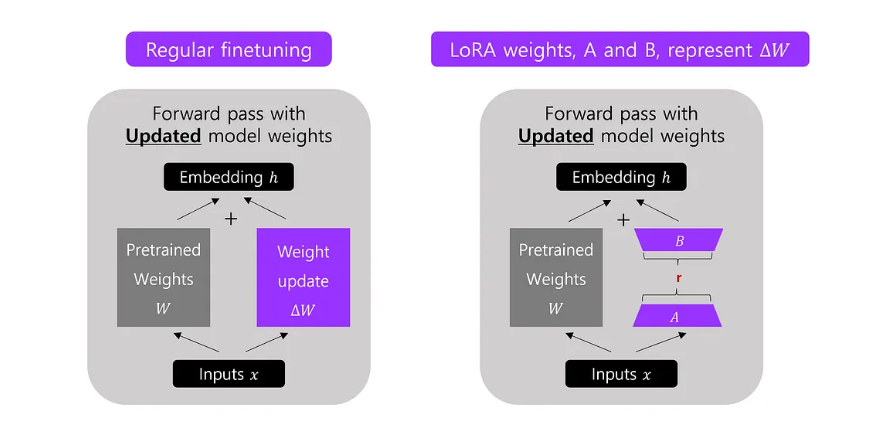
\includegraphics[width=0.8\textwidth]{figures/lora.png}
    \caption{Full Fine-Tuning Vs LoRA}
    \label{fig:lora}
\end{figure}


One popular emerging method that has been developed to achieve this goal is Low-Rank Adaptation (LoRA). This technique injects low-rank matrices into the weight matrices of the transformer layers \cite{pre_ft_ElKhoury2024LLMRecsys}, which serve as the only trainable parameters during fine-tuning. The small proportion of trainable weights enables efficient adaptation with minimal overhead, that both preserves the pre-trained knowledge of the model and adapts to the desired domain. Figure \ref{fig:lora} displays the difference between full fine-tuning and LoRA. An extension of LoRA, Quantized LoRA (QLoRA) further optimizes the fine-tuning process by quantizing the LLM in 4-bit precision. This significantly reduces the memory requirements for training, making it feasible to fine-tune LLMs on consumer-grade GPUs \cite{pre_ft_ElKhoury2024LLMRecsys}.


%==================================================
%==================================================
\subsection{Role in Thesis}

In the context of this thesis, the base model "mistralai/Mistral-7B-Instruct-v0.2" was fine-tuned using QLoRA. In order to lower the memory footprint, we applied 4-bit NF4 quantization and gradient checkpointing, which only stores a few “checkpoint” activations computed during the forward pass of model training. The LoRA configuration contained a rank of 16, a scaling factor of 64, that controls the magnitude of the LoRA update relative to the frozen base model, and a dropout rate of 0.05 to prevent overfitting. A more detailed explanation of the fine-tuned LLM system is presented in section \ref{sec:fine_tuned_llm}.

%==================================================
%==================================================
\subsection{Limitations}

While PEFT techniques significantly enable efficient fine-tuning, the approach of using a single model is prone to several disadvantages. Its main limitation resides in the static nature of the memory of the produced LLM. If we desire to update the knowledge of the model, we are forced to re-train it on updated data. Although the computational cost can be reduced by methods such as QLoRA, fine-tuning remains a time-consuming process we wish to avoid. The fine-tuned model can also suffer from hallucinations, as there is no guarantee that the generated output will always be accurate. To address these challenges, several alternative methods have been developed, such as  Retrieval-Augmented Generation, which we explain in detail below.



%==================================================
%==================================================
%==================================================
\section{Retrieval-Augmented Generation (RAG)}
\label{sec:lit_rag}

Fine-tuning an LLM to adapt to a specific task results in a specialized but relatively static model, prone to hallucinations. Retrieval-Augmented Generation (RAG) is a technique developed to solve these problems by leveraging dynamic knowledge.


%==================================================
%==================================================
\subsection{Introduction to RAG}

RAG is a method that enhances language model generation by incorporating external knowledge. Instead of relying on the memory stored in the model weights, we retrieve relevant information, typically documents or chunks of text, from external sources (e.g. files, databases), and feed it to the LLM to generate the final output \cite{RAG_Kumawat2024}. This approach enables dynamic memory updating, as the knowledge of the model is stored outside of the LLM and can be modified. In addition, it drastically reduces the hallucinations, as the information is retrieved in real time from the outer source and passed to the LLM. Figure \ref{fig:rag_concept} displays the workflow of a RAG system.

\begin{figure}[h]
    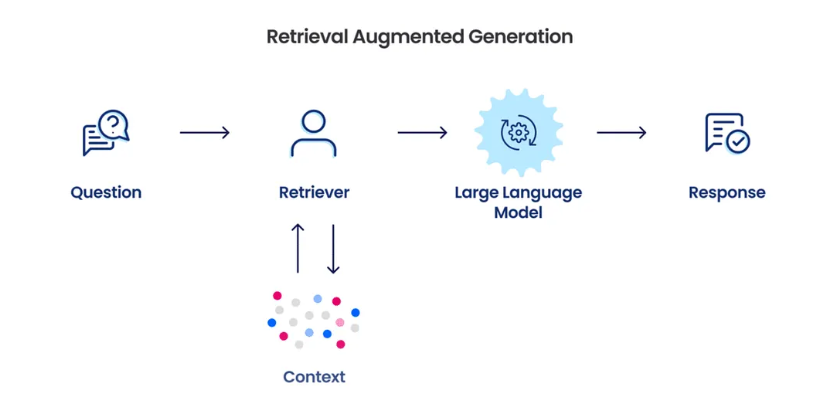
\includegraphics[scale=0.65]{figures/rag_concept.png}
    \centering
    \caption{Retrieval-Augmented Generation Workflow}
    \label{fig:rag_concept}
\end{figure}


%==================================================
%==================================================
\subsection{General RAG Workflow}

The general workflow of a RAG system usually involves two main steps: retrieval and generation, each corresponding to a component, the retriever and the generator, respectively. 

\begin{itemize}
    \item \textbf{Retriever:} Responsible for fetching  relevant information from external knowledge sources. It typically uses an embedder model, which encodes the user rquery in real time, and performs a similarity search with the pre-computed embeddings stored in the sources. The most relevant documents are selected and returned for the generation step.

    \item \textbf{Generator:} A generative Large Language Model that receives the retrieved information and generates a context-aware coherent output. By basing the generation on the retrieved data  the risk of hallucinations is mitigated.
\end{itemize}



%==================================================
%==================================================
\subsection{Role in Thesis}

Within this thesis, the retriever we use is "BAAI/bge-large-en-v1.5". This is a BERT-based encoder with 355 million parameters. The generator we select is "Llama 3" with 8 billion parameters. Before deploying the RAG framework, we apply the embedder on the neighborhood and NACE descriptions to pre-compute their vector representations, so we can simply load them during runtime. The process involves encoding the user query in real-time, performing a similarity search with the NACE embeddings to extract the desired business type, and another similarity search, this time with the neighborhood embeddings, to suggest recommendations that align with user preferences. The selected locations are then fed into the generator along with their descriptions to construct the final user output. A more detailed explanation of the RAG pipeline system is presented in section \ref{sec:rag}.




%==================================================
%==================================================
\subsection{Limitations}

Although utilizing a RAG pipeline addresses certain challenges presented in the fine-tuning approach, it introduces its own set of limitations. Since the pipeline consists of multiple modules, the inference time is bigger, making the system slower. In addition, the structure of the system largely depends on the quality of the retriever and the generator, chaining it to their own weaknesses. Finally, it usually requires additional infrastructure for storing the pre-computed embeddings. 


%==================================================
%==================================================
%==================================================
\section{Introduction to Chatbots}

Chatbots are advanced generative AI models that thrive at understanding and generating human language. Over the recent years, they have undergone a significant change in terms of quality and implementation, due to the emergence of Large Language Models (LLMs) \cite{chatbots_hundertmark2024}. While traditional chatbots used simple keyword-based rules to answer questions, modern chatbots  enhance user experience by leveraging the state-of-the-art NLP ability of LLMs, enabling dynamic request-response conversations with personalized and context-aware responses. This has motivated the application of chatbots to various domains in order to provide new insights and hopefully better accuracy and performance.

While regular LLMs receive a text input and return a text output, the consecutive queries are independent and lack the context of the conversation. A chatbot wraps around an LLM by adding features that essentially transform the LLM into a complete application. The two LLM-based approaches we described in sections \ref{sec:lit_ft} and \ref{sec:lit_rag} are the brain of the system. We will add features such as dialog and memory management, an interface layer, and communication between the frontend and backend components, in order to create a user-friendly chatbot application.

Since chatbots are built upon LLMs, they inherit not only their strengths, but their limitations as well. They are also even harder to evaluate, as their predictions depend on the conversation history.
In the context of this thesis, we aim to integrate a fine-tuned LLM approach and a RAG pipeline into a chatbot application, in order to exploit the advantages and disadvantages of each method.


%==================================================
%==================================================
%==================================================
\section{Summary}

In this chapter, we reviewed the research areas most relevant to the problem of business location recommendations, which form the basis of this thesis. We started by mentioning the motivation behind improving business location recommendation, and how GIS data enhance location analysis by providing geographic and demographic content. Next, we introduced machine learning and its integration with GIS, highlighting how ML models were used as supportive tools for generating proxy ground truths and providing interpretability. NACE codes were presented as a classification technique for economic activities. Moreover, we examined LLMs and domain-specific adaptation through fine-tuning, as well as the RAG framework and its components. Both approaches present different strengths and limitations, which we aim to exploit in the following chapters. Finally, we reviewed the process of transforming a simple LLM-based system into a chatbot application.

    \chapter{Data Collection and Preprocessing}
\label{chap3}

This chapter describes the data collection process and the preprocessing applied to make the data suitable for the models that will be used later. We will start by explaining how the multiple datasets were acquired, then see how they are joined along with the exploratory data analysis of the final dataset, and finally explore how the ground truths of the task were created.

\section{Overview of Data Sources}

The main datasets used in this thesis are the following 3: the Business Entries Dataset, the Municipal Communities Dataset, and the Neighborhoods Dataset. We will start by seeing how each of these was acquired and what preprocessing modification were made to prepare them for their Exploratory Data Analysis and later practical utilization.


%==================================================
%==================================================
\subsection{Business Entries Dataset}

Our first aim was to collect a dataset of business entries across the city of Volos. In order to do this we collected data from multiple sources and via different methods. Below, we will be breaking down each source and the process of merging them.


% ======================================================
\subsubsection{Foursquare (API Retrieval)}

Foursquare is a global platform that provides information about places and human mobility \cite{foursquare}. In order to acquire data from this source, we used its public API. Specifically, we created a grid of points around Volos \ref{fig:centroids} that represent the centroid of overlapping circles, in order to cover the area of the whole city \ref{fig:centroids_with_area}. 

\begin{figure}[htbp]
    \centering
    \begin{minipage}[b]{0.45\textwidth}
        \centering
        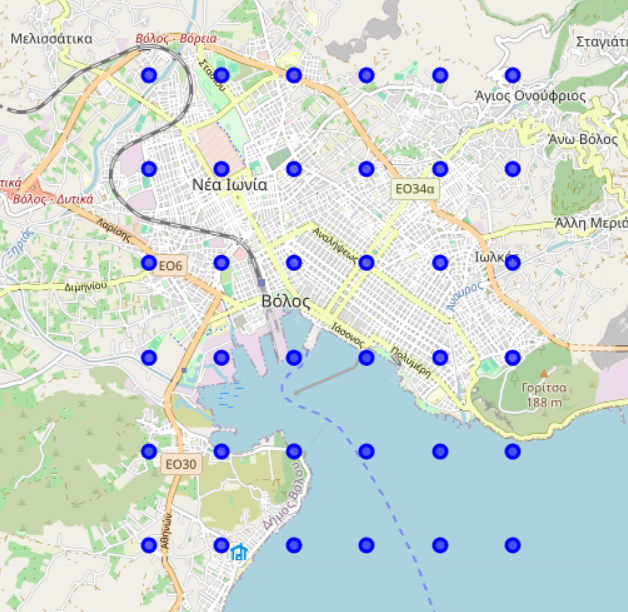
\includegraphics[height=5cm]{figures/centroids.png}
        \caption{Grid Centroids}
        \label{fig:centroids}
    \end{minipage}
    \hfill
    \begin{minipage}[b]{0.45\textwidth}
        \centering
        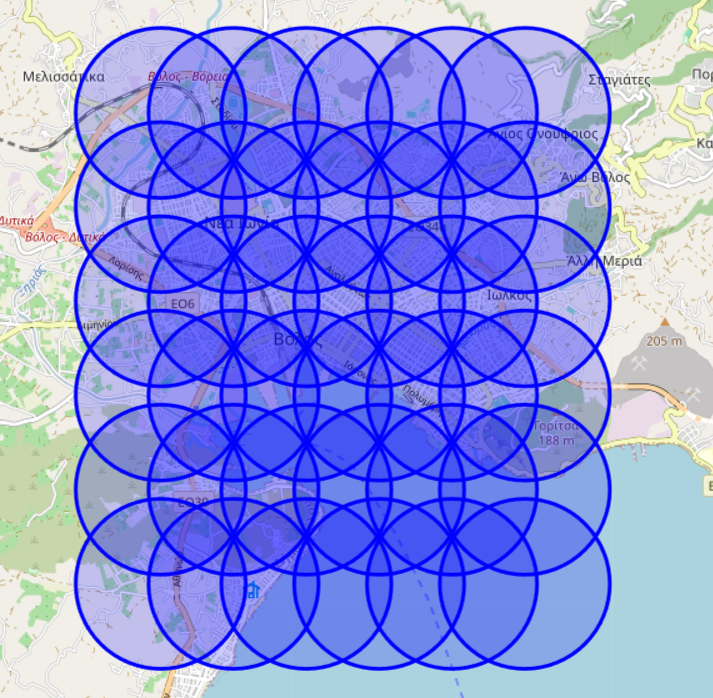
\includegraphics[height=5cm]{figures/centroids_with_area.png}
        \caption{Total Area Covered}
        \label{fig:centroids_with_area}
    \end{minipage}
\end{figure}


An API call was made for each circular area and the results were stored in a JSON file ('places\_\{i\}.json'). Then, we merged the results and deleted the duplicates that occurred due to the area overlapping, and ended up with the final JSON file ('all\_places\_deduplicated.json'). Finally, we transformed the json file into a CSV file in order for the entries to later be able to merge with entries from other sources ('foursquare\_data.csv'). This final file also contains the features 'Rating' and 'Reviews' which we manually added via the Foursquare API for each entry, and also the feature 'Postal Code' that was acquired via the Google Maps API. The total entries of this source were 307. The structure of the Foursquare entries was the following: Name, Address, Rating, City, Postal Code, Latitude, Longitude, Category, Country, Reviews.

%==================================================
\subsubsection{Xrysos Odigos (Web Scraping)}

Xrysos Odigos (Yellow Pages) is a website that contains information about businesses of various categories across Greece \cite{xrysos_odigos}. In order to collect data from this source, the Web Scraper Chrome Extension was used. The raw entries acquired were initially 4364. This source did not provide the 'Latitude' and 'Longitude' features, therefore we performed geocoding through the Google Maps API. The method was successful for 3420/4364 of the entries, so the remaining coordinates were inserted manually, using the Google Maps App. The data was saved in a CSV file ('xrysos-odigos-volos-ratings.csv'). The structure of the Xrysos Odigos entries was the following: Name, Address, Rating, City, Postal Code, Latitude, Longitude, Category, Country, Reviews, Description, Phone.

%==================================================
\subsubsection{Greek Catalog (Web scraping)}

Greek Catalog is an online business directory for Greece, similar to Xrysos Odigos \cite{greek_catalog}. In order to collect data from this source, we utilized the Web Scraper Chrome Extension once more. The raw entries collected were 46 this time. This source did not provide the 'Postal Code' feature, therefore we performed geocoding through the Google Maps API. The data was saved in a CSV file ('greek-catalog-volos.csv'). The structure of the Greek Catalog entries was the following: Name, Address, Rating, City, Postal Code, Latitude, Longitude, Category, Country, Reviews.

%==================================================
\subsubsection{Vacation Renter (Web scraping)}

Vacation Renter is a travel accommodation aggregator that aggregates hotel listings from multiple booking platforms (Booking.com, Vrbo, etc.) \cite{vacation_renter}. In order to collect data from this source, the Web Scraper Chrome Extension was used one final time. The raw entries acquired were 24. This source did not provide the 'Latitude', 'Longitude' and 'Postal Code' features either, therefore the Google Maps API as used to perform geocoding one final time. The 'Category' features was also set to 'Hotel' since this source specifies on this sector. The data was saved in a CSV file ('vacation-renter-volos.csv'). The structure of the data was the following: Name, Address, Rating, City, Postal Code, Latitude, Longitude, Category, Country, Description, Features.

\begin{table}[h!]
    \centering
    \caption{Attribute Presence Across Sources (highlighted were kept)}
    \begin{tabular}{lcccc}
    \toprule
    \textbf{Attribute} & \textbf{Foursquare} & \textbf{Xrysos Odigos} & \textbf{Greek Catalog} & \textbf{Vacation Renter} \\
    \midrule
    \rowcolor{yellow!20}
    Name              & \cmark & \cmark & \cmark & \cmark \\
    \rowcolor{yellow!20}
    Address           & \cmark & \cmark & \cmark & \cmark \\
    \rowcolor{yellow!20}
    Rating            & \cmark & \cmark & \cmark & \cmark \\
    \rowcolor{yellow!20}
    City              & \cmark & \cmark & \cmark & \cmark \\
    \rowcolor{yellow!20}
    Postal Code       & \cmark & \cmark & \cmark & \cmark \\
    \rowcolor{yellow!20}
    Latitude/Longitude& \cmark & \cmark & \cmark & \cmark \\
    \rowcolor{yellow!20}
    Category          & \cmark & \cmark & \cmark & \cmark \\
    \rowcolor{yellow!20}
    Country           & \cmark & \cmark & \cmark & \cmark \\
    \rowcolor{yellow!20}
    Reviews           & \cmark & \cmark & \cmark & -- \\
    \rowcolor{yellow!20}
    Description       & --     & \cmark & --     & \cmark \\
    Phone             & --     & \cmark & --     & -- \\
    Features          & --     & --     & --     & \cmark \\
    Number of Entries & 307    & 4364   & 46     & 24 \\
    \bottomrule
    \end{tabular}
\end{table}

%==================================================
\subsubsection{Merging the Business Data Sources}


On the table below, we can see a review of the structure of the individual data collected from the multiple sources mentioned above, as it has already been modified in order to facilitate their merging. Since the 'Phone' and 'Features' columns only exist in one dataset, we decided to drop them. Regarding the features 'Description' and 'Reviews' which are now the only missing features on some datasets, we simply set their values to Nan in these cases. The actual merging is simple, since all the individual datasets now comprise of the same structure. I ended up with a total of 307 + 4364 + 46 + 24 = 4741 entries, and 11 features.

\begin{figure}[t]
    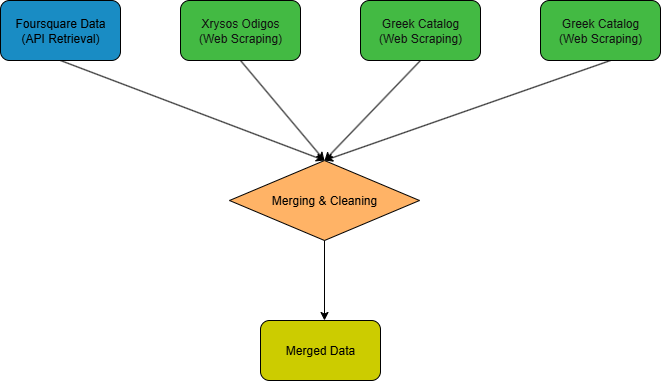
\includegraphics[scale=0.4]{figures/data_merging.png}
    \centering
    \caption{Merging \& Cleaning the Business Data}
    \label{data_merging_cleaning}
\end{figure}

\newpage

%==================================================
\subsubsection{Cleaning the Merged Business Dataset}
Following the concatenation of the individual business datasets, a cleaning process was applied to ensure the final dataset’s integrity and uniformity. Initially, 10 duplicates across the different datasets were identified and deleted. The 'Description' feature, that previously contained unintended line breaks, was reformatted for consistency. A total of 400 entries were found to not actually be located within the administrative boundaries of Volos, and therefore they were eliminated. After verifying the geographical accuracy, some wrongly performed Geocodings were corrected, either manually, or programatically via the Google Maps API, and 1 problematic entry was deleted. 

Multiple entries lacked addresses, so we managed to find and manually insert a proportion, but deleted the 26 remaining. We also excluded 390 records lacking both address and geographic coordinates. Regarding the missing values of the feature 'Postal Code', we manually added them when they were available and removed 3 invalid entries. The feature 'City' also lacked 24 values, which we simply filled with "Βόλος Μαγνησίας". Finally, 4 'Category' values were missing, so we manually inserted them, and deleted 1 invalid record.

Summing up all the records deleted in the cleaning process, we count: 10 + 400 + 1 + 26 + 390 + 3 + 1 = 831, and removing those from the original 4741 we are left with 3910 entries so far.


%==================================================
%==================================================
\subsection{Municipal Communities Dataset}

The next main dataset is the Municipal Communities Dataset. This information was gathered through the ELSTAT platform. This paragraph presents the process of acquiring the raw data and its preprocessing, leading to the creation of the final Municipal Communities Dataset.


%==================================================
\subsubsection{Data Acquisition (ELSTAT)}

ELSTAT is the official national statistics service of Greece \cite{ELSTAT}. It provides detailed demographic, social, and economic data at various administrative levels. Since the final model's recommendations are expected to be areas within Volos, we searched for the smallest geographic unit with available public datasets in ELSTAT. These units were the Municipal Communities, and we kept the ones within the boundaries of Magnesia (76). The platform provided demographic and economic information for each of them.

\begin{figure}[h]
    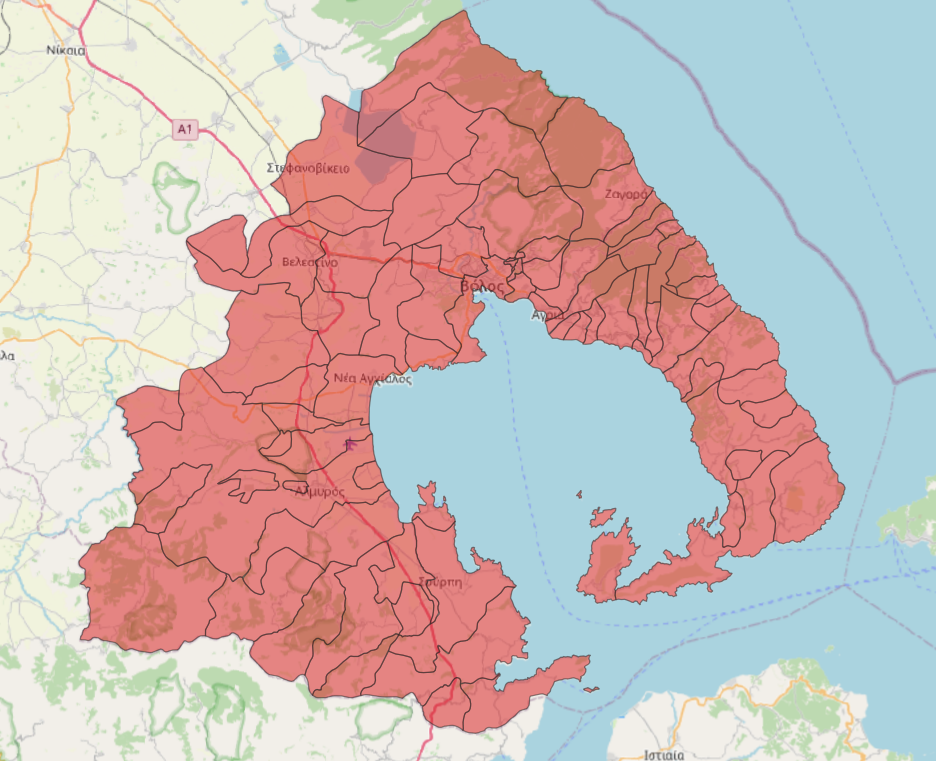
\includegraphics[scale=0.45]{figures/municipal_communities_magnesia.png}
    \centering
    \caption{Municipal Communities within Magnesia}
    \label{municipal_communities_magnesia}
\end{figure}


The demographic data \ref{tab:demographic_columns} contain the population count of each record, along with information about age, educational and marital status groups. More precisely, the age groups are divided to five-year intervals, while the education levels are categorized into six levels. Marital status is recorded as single, married, widowed, or divorced. The total features provided are 32.

The economic features acquired from the ELSTAT platform \ref{tab:economic_columns} are organized hierarchically. The root feature 'Σύνολο' is divided into 'Οικονομικά ενεργοί' and 'Οικονομικά μη ενεργοί'. 'Οικονομικά ενεργοί' is further categorized into 'Άνεργοι' and 'Απασχολούμενοι', while the latter is finally splitted into 'Πρωτογενής', 'Δευτερογενής', 'Τριτογενής'. The total features provided are 12.

The merging of demographic and economic features was simple, since they reference the same municipal community records. The economic and demographic datasets had 4 features in common ('ΠΕΡΙΦΕΡΕΙΑΚΗ ΕΝΟΤΗΤΑ', 'ΔΗΜΟΣ', 'ΔΗΜΟΤΙΚΗ ΕΝΟΤΗΤΑ', 'ΔΗΜΟΤΙΚΗ ΚΟΙΝΟΤΗΤΑ'), so the total number of features ended up being 32 + 12 - 4 = 40. The shape of the dataset is therefore 76x40 so far.


%==================================================
\subsubsection{Feature Engineering}

After merging the demographic and economic datasets, preprocessing steps were applied to guide the feature selection and engineering so the final dataset is enhanced for later analysis. The first transformation applied was to normalize the raw count values for the demographic features of age, education, and marital status groups. This is done to put the features on a comparable scale and to be better fitted for their eventual integration with machine learning models, which benefit from normalized scales.\\

\begin{figure}[H]
    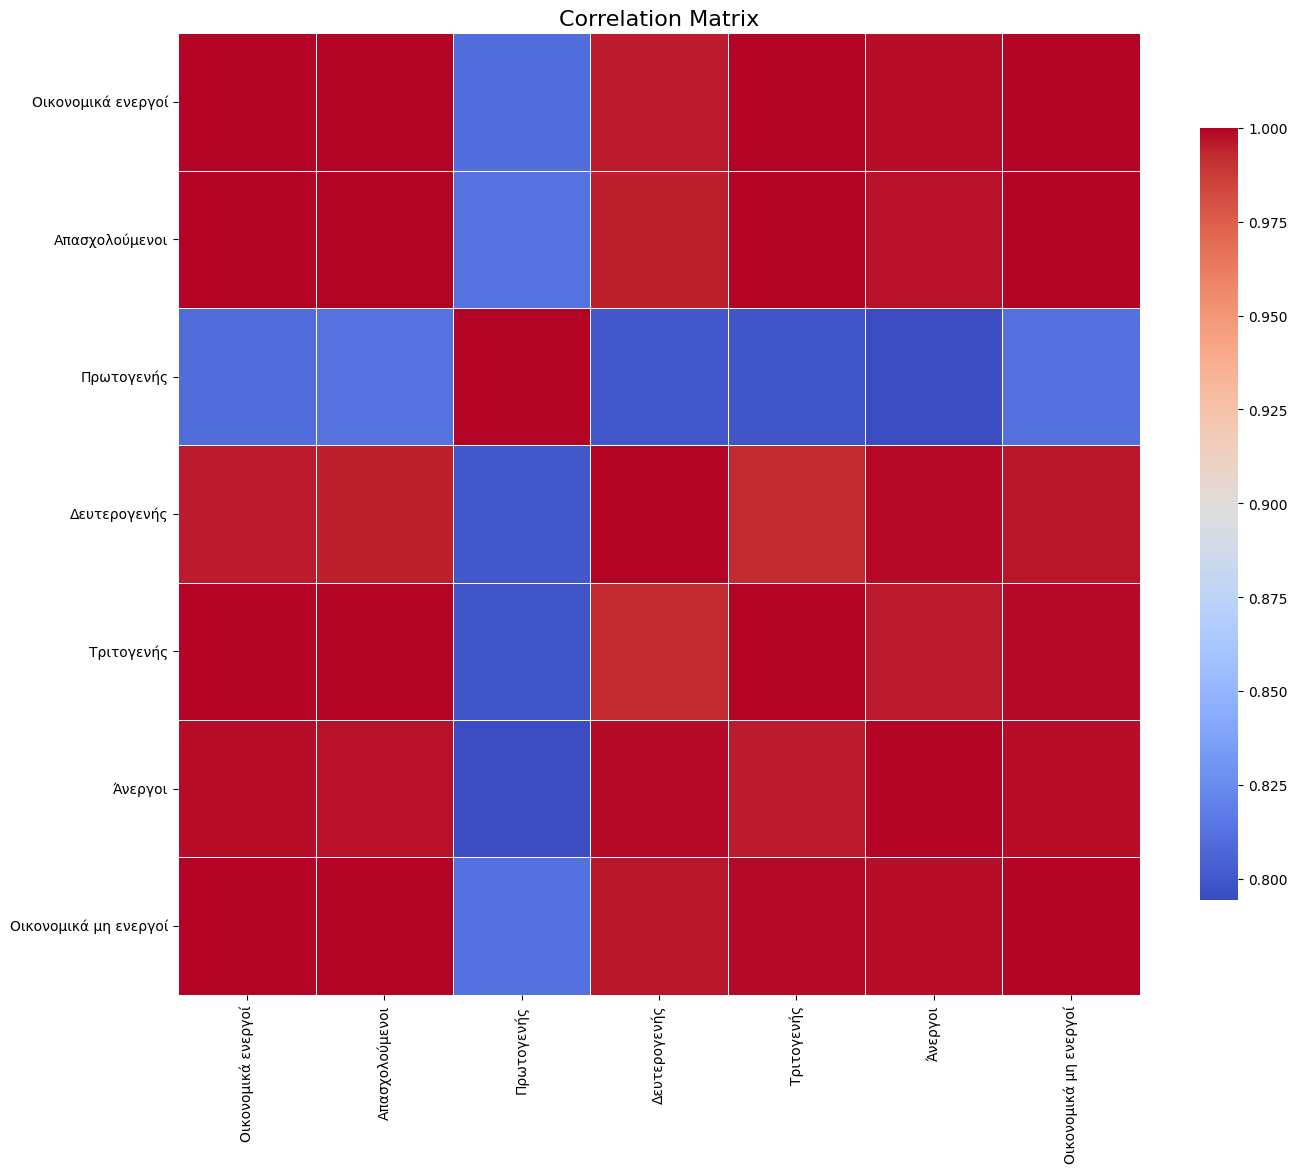
\includegraphics[scale=0.3]{figures/multicoll4.png}
    \centering
    \caption{Correlation Matrix of Economic Features}
    \label{multicollinearity_economic}
\end{figure}

The raw economic features were organized hierarchically, meaning that they contained redundant information. This can be verified by applying a correlation matrix that demonstrates their strong multicollinearity \ref{multicollinearity_economic}. Therefore, we used them to extract some meaningful economic features, like unemployment rate, labor force participation rate, and primary, secondary, and tertiary sector rate. The equations used to extract them from the old features are described in \ref{sec:elstat_feature_engineering}.

In order to reduce the dimensionality of the dataset, we narrowed down the features within age ($15 \rightarrow 3$), educational level ($6 \rightarrow 3$) and economic feature groups ($8 \rightarrow 5$) \ref{sec:elstat_feature_engineering}. The old features were eliminated. The marital status group was not changed. 

In addition, the feature 'Area\_km2' was added through the use of QGIS, which represents the total land area of the municipal community measured in square kilometers. This was possible because, apart from their tabular data, ELSTAT also provided the shapefiles for the geographical units.

I also added a feature with the English name of the Municipal Communities. The final Municipal Communities Dataset has 76 entries and  22 features \ref{tab:final_municipal_communities_columns}.


%==================================================
%==================================================
\subsection{Neighborhoods Dataset}

While the Municipal Community level data are indeed useful, their unit's size is large for the task we aim to achieve. Ideally, we would like smaller geographical units to represent the candidate locations. Therefore, we also created the Neighborhoods Dataset. This paragraph presents the process of acquiring data on the neighborhood level.


%==================================================
\subsubsection{Data Acquisition (QGIS)}

QGIS (Quantum Geographic Information System) is a free and open-source GIS software used for viewing, editing, and analyzing geospatial data \cite{QGIS}. To help acquire spatial data, it provides a QuickOSM plugin, which allows querying and downloading OpenStreetMap data based on specific tags and spatial filters. We used multiple filters (neighborhoods/villages/suburbs/...) to make queries within Volos and therefore received multiple layers, both of point and polygon type. After processing them, we merged them into 1 point layer and stored them as a shapefile ('merged\_neighborhood\_points.shp').

In order for each business entry to be able to be matched to its corresponding neighborhood later, the shapefile should also possess a geomgetry attribute. To achieve this we applied Voronoi Polygons to transform the Point Layer to a Polygon Layer and saved it into another shapefile ('final\_voronoi\_output.gpkg'). The Voronoi Polygons tool partitions space into regions such that every location within a polygon is closer to its generating point (in this case, the neighborhood point layer) than to any other point \cite{Voronoi_polygons}. In \ref{neighborhoods_magnesia} we can see the initial point layer and the produced polygon layer.\\


\begin{figure}[h]
    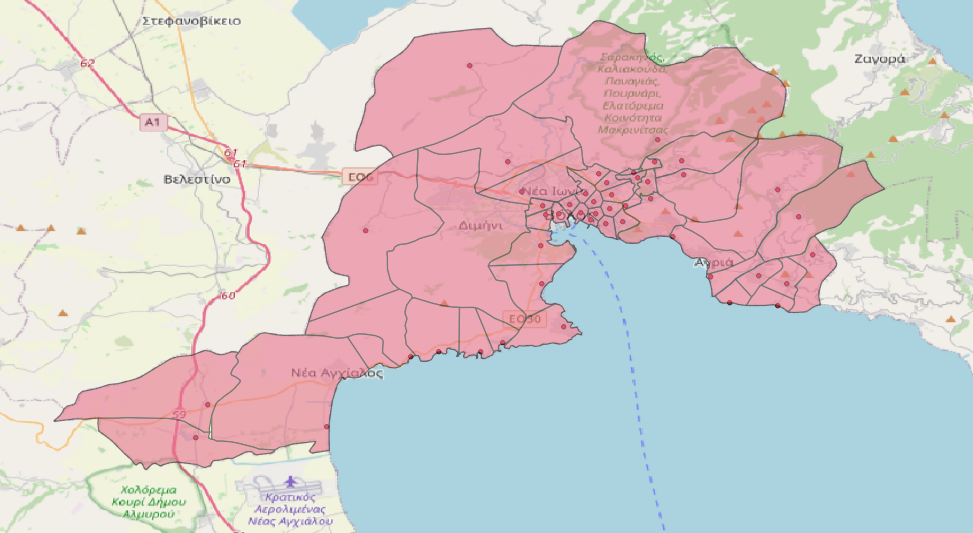
\includegraphics[scale=0.6]{figures/neighborhoods_magnesia.png}
    \centering
    \caption{Neighborhoods within Magnesia}
    \label{neighborhoods_magnesia}
\end{figure}


%==================================================
\subsubsection{Feature Engineering}

Next, we followed a feature enhancement process, that provided some additional features by utilizing QGIS. We were able to extract the centroid coordinates ('x\_centroid', 'y\_centroid') and the polygon area ('area\_km2') for each neighborhood.

We also collected the distance of every neighborhood from various Points Of Interest (POIs). The city center and the port were represented by fixed points, so the distance of each neighborhood to these POIs was measured as the distance between those fixed points and the neighborhood centroids.

Certain POIs, such as main roads, transport stations, and universities, are represented by multiple points or lines. Consequently, I used the QuickOSM plugin to extract a shapefile for these cases. Then, for each neighborhood centroid, the nearest geometry was identified using the 'geopy' library. The final form of the Neighborhood dataset consists of 48 entries with 11 features so far \ref{tab:neighborhood_columns}.


%==================================================
%==================================================
%==================================================
\section{Datasets Integration}


In the previous section, we analyzed how the 3 main datasets were created. In this section, we will see how they are integrated with each other and how the total features end up being greatly enriched in comparison to the initial business dataset. We will start by showing how the NACE code is assigned to each business and then see how we join it with its corresponding municipal community and neighborhood.


%==================================================
\subsection{NACE Code Integration}

In order to standardize business activity classification, the next step was the integration of the NACE code for each business entry. The workflow for this task involved the isolation of all the unique "Category" feature values, and their mapping to their corresponding NACE code. This mapping was performed manually to ensure accuracy, given the variability in category naming across sources. Once it was completed, it was joined with the merged dataset, to add the NACE code and description to each record. In the course of the aforementioned process 4 invalid entries were spotted and deleted, leading to the final number of business records being 3906. 


\begin{figure}[h]
    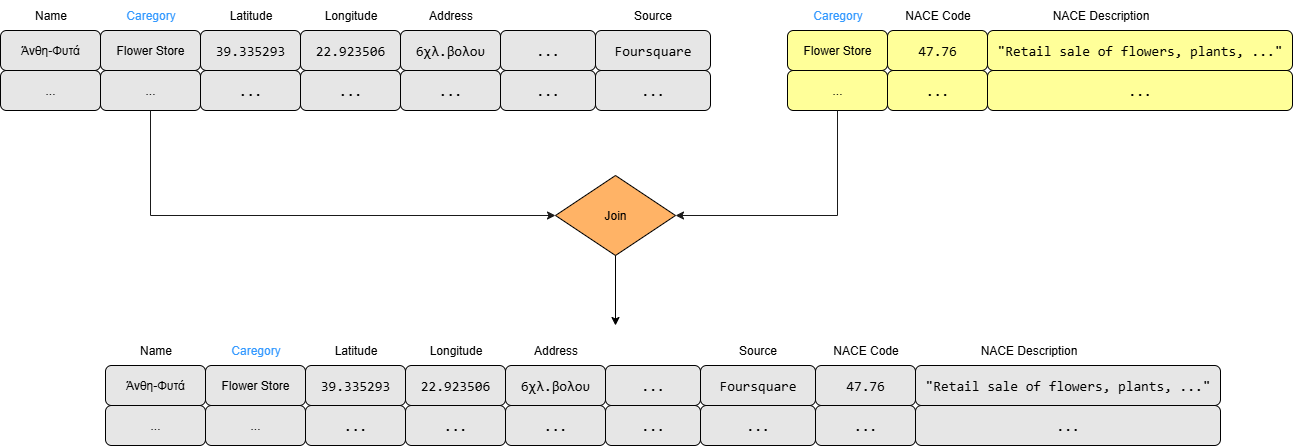
\includegraphics[scale=0.35]{figures/business_nace_join.png}
    \centering
    \caption{Integrating NACE code to the Business Data}
    \label{data_nace_integration}
\end{figure}


Since we added these 2 features, plus we added a 'Source' feature that identifies where I extracted the specific entry from, the shape of the final business dataset is: 3906 entries and 14 columns \ref{tab:business_columns}.


%==================================================
\subsection{Municipal Communities Integration}

Next, we integrated the business entries with the Municipal Communities Dataset. This process consists of two steps: assigning every business to its corresponding municipal community, and merging on this value with the other dataset. The first step was implemented by performing a spatial join between the business dataset and the polygon layer of Municipal Communities programmatically \cite{geopandas_sjoin}. After adding the 'Municipal Community' feature to every entry, we simply join the 2 datasets on it.

\begin{figure}[h]
    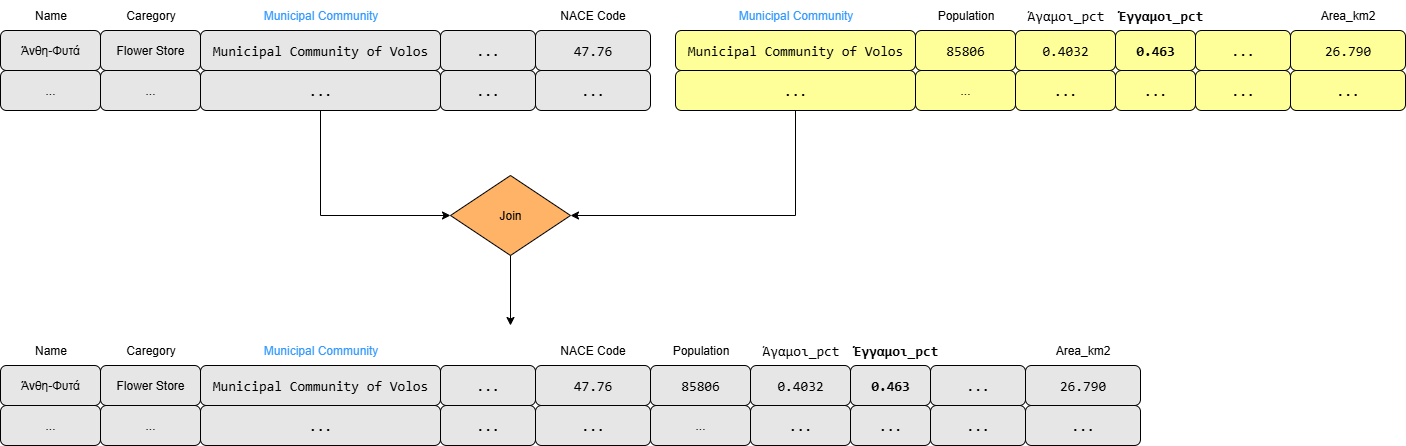
\includegraphics[scale=0.3]{figures/business_mc_join.png}
    \centering
    \caption{Integrating Municipal Community Features to the Business Data}
    \label{data_mc_integration}
\end{figure}

The important part of this process was the 1st step, essentially the enhancement of the business data without necessarily joining the 2 datasets, since this can be done at any time later. The number of entries remains 3906, and the number of features of just the business data is 15 since we just added the 'Municipal Community' feature. If we want to inspect the total features of the joined set, they are 36 since we added the 22 features of the municipal community, and we dropped 'ΔΗΜΟΤΙΚΗ ΚΟΙΝΟΤΗΤΑ ΕΛΛ' as keeping the Greek name was unnecessary.


%==================================================
\subsection{Neighborhoods Integration}

The workflow followed on this paragraph perfectly mirrors the previous one. We perform another spatial join \cite{geopandas_sjoin}, this time assigning each business to its corresponding neighborhood. The spatial join failed for 24 entries because all the neighborhoods belong to the municipality of Volos, while these specific businesses did not, so they were deleted. The valid entries can now be joined to acquire the Neighborhood Dataset features.

\begin{figure}[h]
    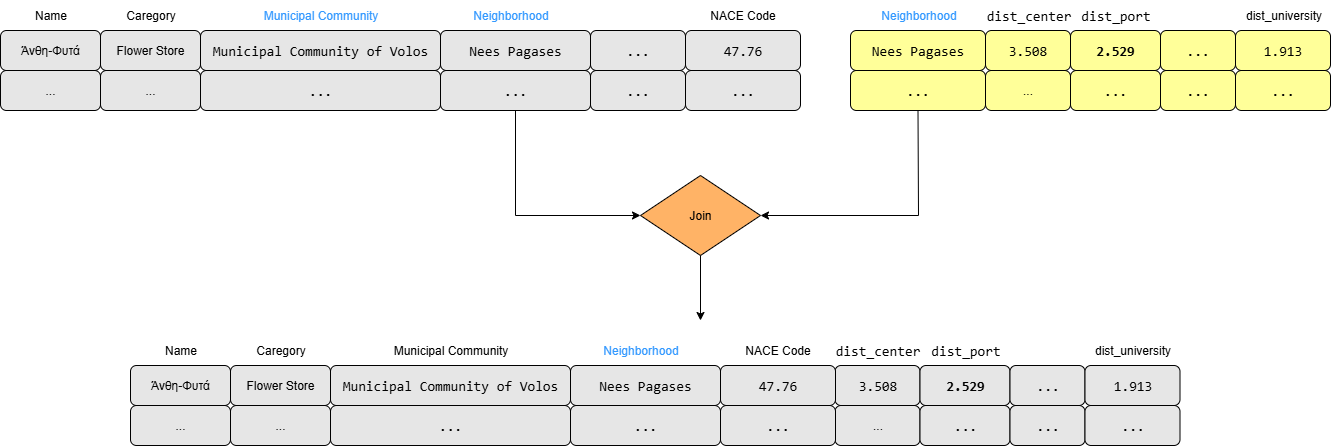
\includegraphics[scale=0.3]{figures/business_neigh_join.png}
    \centering
    \caption{Integrating Neighborhood Features to the Business Data}
    \label{data_neigh_integration}
\end{figure}

As was the case above, the important improvement through this process was the integration of the 'Neighborhood' feature on the business entries. The shape of the business dataset is now 3882 records, due to the 24 invalid spatial joins, and 16 columns since adding 'Neighborhood'. If we look at the fully joined dataset, after joining both on the 'Municipal Community' and 'Neighborhood' features, and keeping only the useful columns for a business entry (dropping 'Geometry', 'Centroid\_x','Centroid\_y', 'Neighborhood\_Greek','ΔΗΜΟΤΙΚΗ ΚΟΙΝΟΤΗΤΑ ΕΛΛ'), their number is 42. In we can see the final schema of the relationships of the 3 main datasets.


%==================================================
\subsection{Integrating Municipal Communities to Neighborhoods}

In the previous two sections we saw how we connect an individual business to its municipal community and neighborhood. However, there is also a connection between the two geographical units themselves, since each neighborhood essentially lies within a municipal community. We can also add the 'Municipal Community' feature to the Neighborhood Dataset by performing a spatial join \cite{geopandas_sjoin} on its centroids with the municipal communities. The added feature results in a 48x12 shape for the neighborhood dataset. After we do this, we can join the neighborhood with the features of its corresponding municipal community. In \ref{data_connection} we can see the final relationship of the 3 main datasets. The arrows act as foreign keys that allow joining on the specific features.


\begin{figure}[h]
    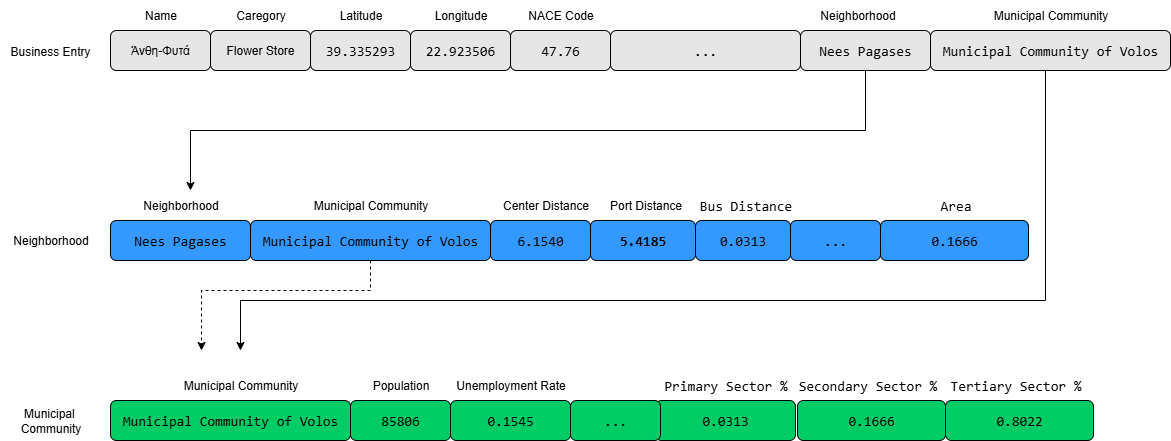
\includegraphics[scale=0.4]{figures/datasets_connected.png}
    \centering
    \caption{Relations of the 3 Datasets}
    \label{data_connection}
\end{figure}


%==================================================
%==================================================
%==================================================
\section{Exploratory Data Analysis}

In the previous sections, we described how we obtained the 3 main datasets and how they are related in order to be joined. In the current paragraph, we will analyze the 3 main datasets individually and then the final joined dataset.


%==================================================
\subsection{EDA - Business Dataset (before joining)}
\label{EDA_business}



We started by inspecting the features of the pure business dataset, before joining it with the other ones. As we mentioned previously, the shape of this dataset is 3882x16. Most of its features are spatial as they provide information about its location. As is obvious, all entries in the 'Country' field are set to 'Greece'. The overwhelming majority of the 'City' column contains the value 'Βόλος Μαγνησίας' (82.86\%), while the next most frequent value is 'Νέα Ιωνία Μαγνησίας' (11.23\%) \ref{fig:city_distr}. The entries contain 12 unique 'Postal Code' values, with '38221', '38333' and '38334' being the most common \ref{fig:postal_distr}. In \ref{business_map_clustered} we can see a clustered version of the businesses on a map, as specifying every point would hinder the clarity of the visualization. We see that most records are located within the city center.

\begin{figure}[h]
    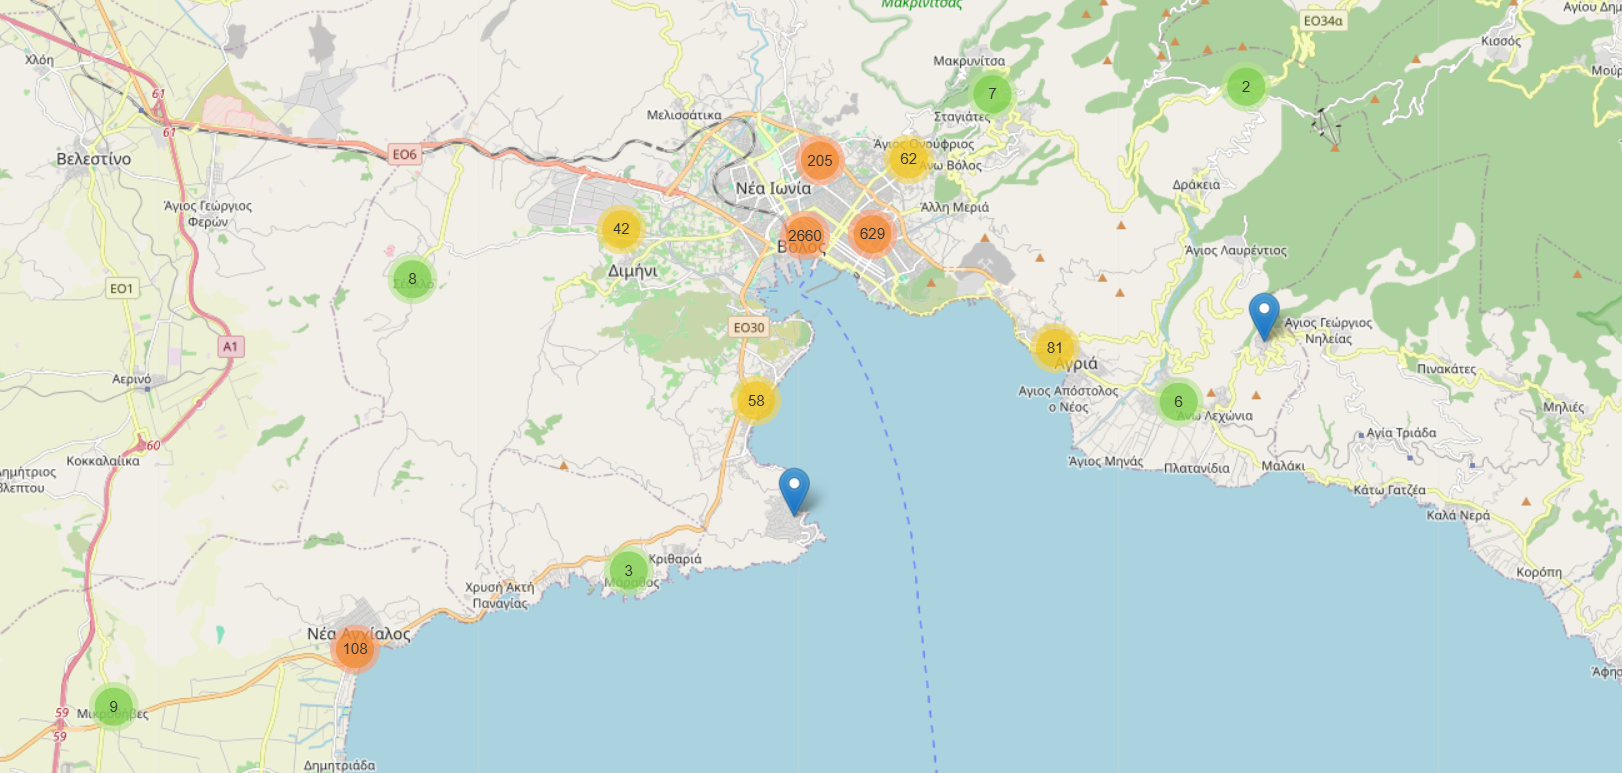
\includegraphics[scale=0.45]{figures/map_clustered.png}
    \centering
    \caption{Clustered Businesses Visualization}
    \label{business_map_clustered}
\end{figure}

\begin{figure}[h]
    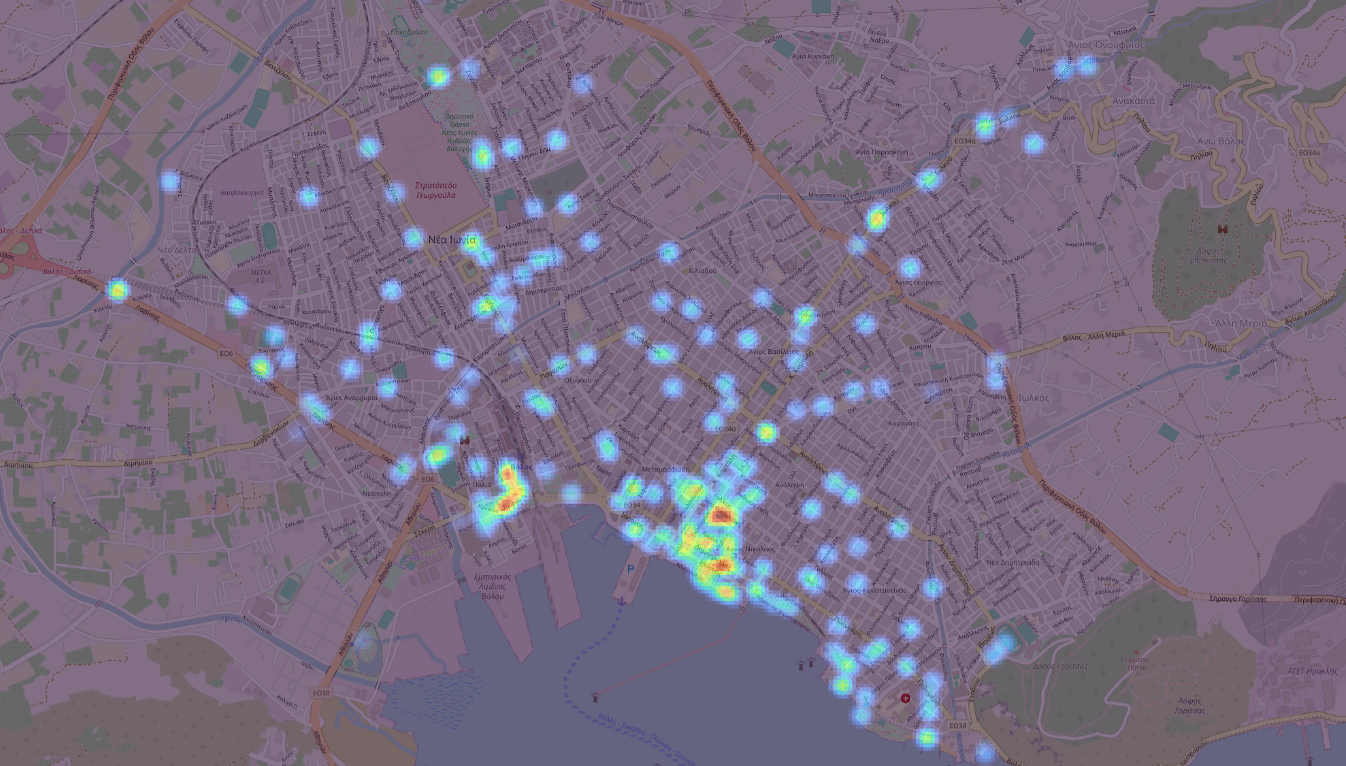
\includegraphics[scale=0.5]{figures/ratings_heatmaps.png}
    \centering
    \caption{'Rating' Feature Heatmap}
    \label{fig:heatmap}
\end{figure}

Although the 'Rating' values are extremely sparse (only 5.87\% present), the distribution of their values is right-skewed \ref{fig:distr_rating}. The figure \ref{fig:heatmap} shows a heat map of the ratings in the city, highlighting their highest values mainly in the center and the Palaia area. Regarding the categorization of the business type, the 'Category' feature consisted of 1233 unique values \ref{fig:category_distr}, while the 'NACE Code' feature only had 306. This is expected since the categogies were the raw values we acquired along with the business entries, while the official categorization method that we will use throughout this thesis is the NACE protocol. In \ref{fig:distr_nace_desc} we can see the most frequent of business types, based on the NACE Code Description. We see that they comprise medical activities, food service and beverage activities, education, and more.

\begin{figure}[h]
    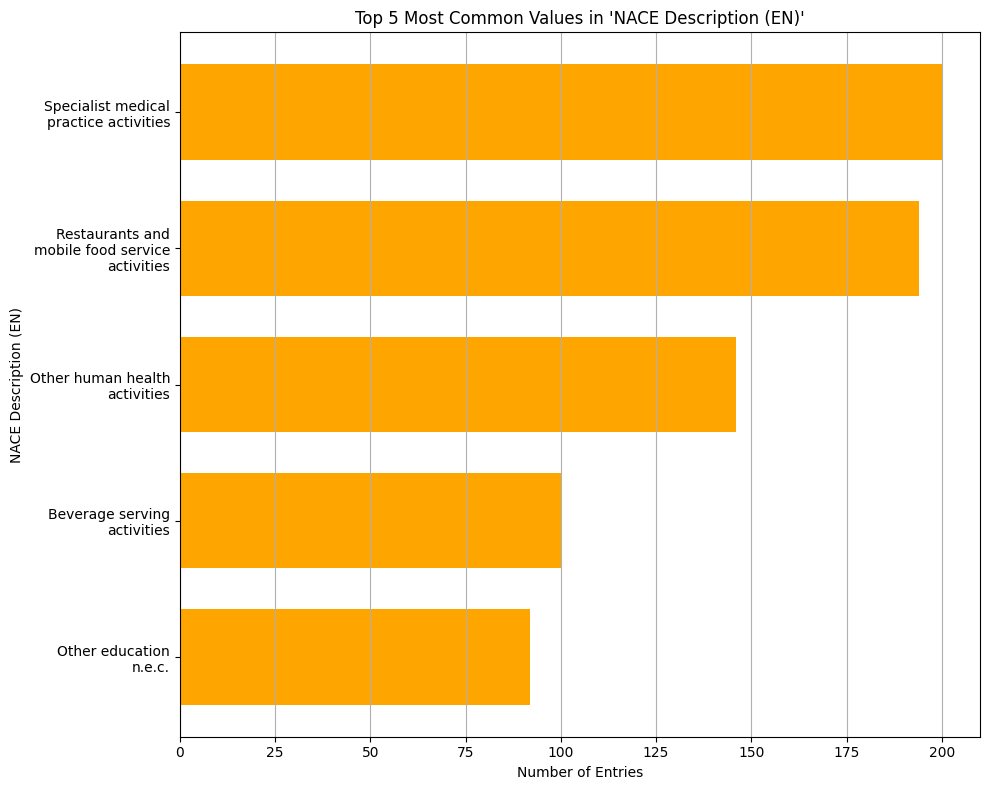
\includegraphics[scale=0.4]{figures/distribution_nace_desc.png}
    \centering
    \caption{'NACE Code' Bar Chart}
    \label{fig:distr_nace_desc}
\end{figure}

Finally, looking into the 'Neighborhood' feature, we can see that its distribution \ref{fig:neighborhood_distr} is much less skewed than the one of 'Municipal Community' \ref{fig:mc_distr}. This is logical because the latter feature refers to a much larger geographical unit which contains the majority of the businesses. The neighborhoods provide a better and informative separation of the areas, and this is why they will be used as the candidates of the recommendation system.  



%==================================================

\subsection{EDA - Municipal Communities Dataset}
\label{EDA_mc}

Subsequently, the Municipal Communities dataset was analyzed, which consists of 76 entries with 23 features. Although 75\% of the spatial units host fewer than 902 people, the municipal communities of Volos and Nea Ionia are outliers, hosting 85.806 and 31.683 respectively. Figure \ref{fig:population_hist} demonstrates the value distribution of the feature, after having removed the 2 extreme outliers mentioned to provide a better visualization. The 'Area\_km2' also contains outliers \ref{fig:box_area}. An attempt was made to identify a correlation between the population and the area features, no sufficient statistical evidence existed to assume such a relationship. The distribution of 'unemployment\_rate' visually suggests a normal distribution approximation. Several statistical tests were applied and did not reject this suspicion while a QQ-Plot strengthened it \ref{fig:stat_unemployment}.

\begin{figure}[h]
    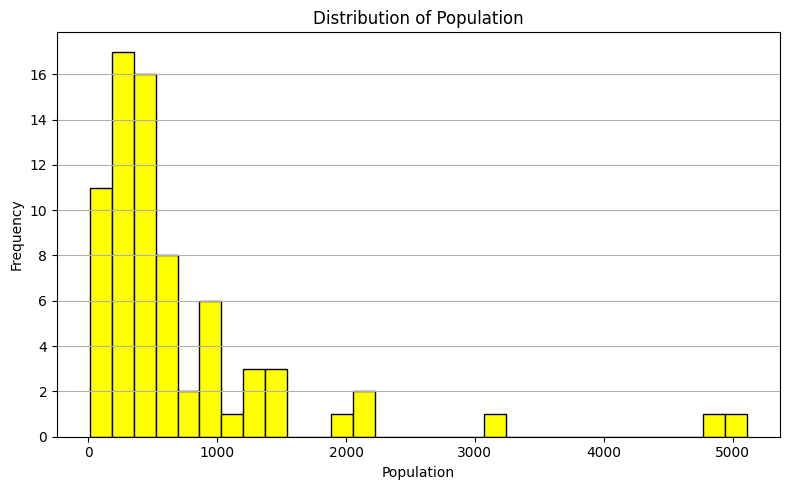
\includegraphics[scale=0.45]{figures/distribution_population_hist2.png}
    \centering
    \caption{'Population' Feature Histogram}
    \label{fig:population_hist}
\end{figure}



The age, education level, marriage and economic sector groups columns comprise feature subsets that suffer internally from multicollinearity since they are perfectly linearly dependent (\ref{fig:corr_age}, \ref{fig:corr_education}, \ref{fig:corr_marriage}, \ref{fig:corr_sector}). Specifically, the percentages of high and low education exhibit a strong negative correlation, as do the percentages of married and unmarried individuals, and the shares of the primary and tertiary sectors. Examining the mean age feature values across all municipal communities shows that the majority of the population is between 10 and 65 years of age \ref{fig:bar_age_mean}. In addition, on average, the majority of the community people posess a low educational level, and higher education levels become progressively less common.
\ref{fig:bar_education_mean}. The mean percentages of married and unmarried citizens correspond to approximately 48.89\% and 35.93\% respectively. Most people are employed in the tertiary sector, followed by the primary and then the secondary sector \ref{fig:bar_sector_mean}.

There is a moderate negative correlation between the 'Population' and the 'age\_65\_plus' columns, which indicates that the most populated municipal communities consist of fewer older people \ref{fig:scat_pop_elderly}. Another relationship I identified was between the unemployment rate and the education level. In particular, it presented a positive correlation with higher education levels \ref{fig:scat_unemployment_high} and a negative correlation with lower education levels \ref{fig:scatter_unemployment_lowed}, both indicating that areas with higher education correspond to lower employment rates. Finally, there is a positive relationship between the proportion of citizens aged 15–64 and labor force participation, which is expected since this age group constitutes the working-age population. \ref{fig:scat_labor_working}.

\begin{figure}[h]
    \centering
    \begin{minipage}[b]{0.45\textwidth}
        \centering
        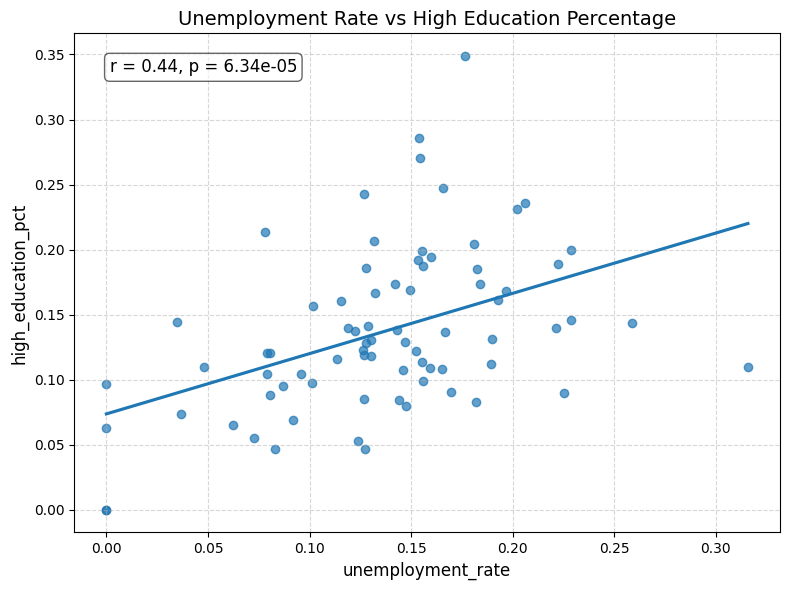
\includegraphics[height=5cm]{figures/scatter_unemployment_highed.png}
        \caption{Scatter Plot: Unemployment Rate VS High Education Level}
        \label{fig:scat_unemployment_high}
    \end{minipage}
    \hfill
    \begin{minipage}[b]{0.45\textwidth}
        \centering
        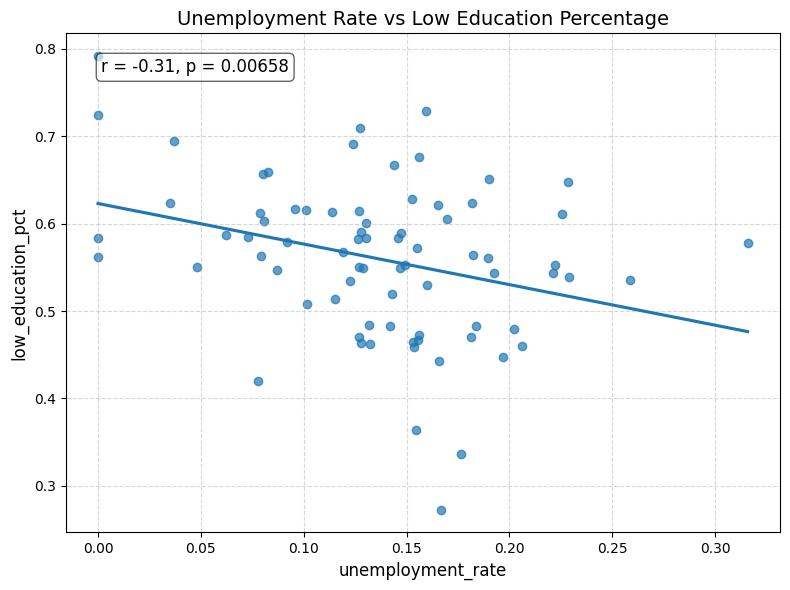
\includegraphics[height=5cm]{figures/scatter_unemployment_lowed.png}
        \caption{Scatter Plot: Unemployment Rate VS Low Education Level}
        \label{fig:scatter_unemployment_lowed}
    \end{minipage}
\end{figure}

%==================================================
\subsection{EDA - Neighborhoods Dataset}


Next, we explored the features of the Neighborhoods Dataset, which consists of 48 entries and 12 total columns. The 'Neighborhood\_Area\_km2' column represents the area of each neighborhood and contains more outliers than the municipal community area \ref{fig:box_area_neigh}. This is caused by the large number of small neighborhoods, particularly those located near the city center, while simultaneously peripheral areas are divided into fewer segments, as we can see in Figure\ref{neighborhoods_magnesia}. The largest areas—Makrinitsa, Glafyra, Dimini, Dimitriada, and Sesklo—also appear as outliers \ref{fig:bar_area_neigh}.

Regarding the distance from the city center, Agios Vasilios, Analipsi, Metamorfosi, Agios Nikolaos and Epta Platania - Oksigono are the most central neighborhoods \ref{fig:bar_center_neigh}. After inspecting the relationship of the neighborhood distance from the city center with various other features, we identified that it presents a positive correlation with many of them. A weak but statistically significant positive relationship with the distance from main roads \ref{fig:scatter_center_highway} confirms the suspicion that central areas tend to have more highways. Its moderate correlation with the distance from transport stops \ref{fig:scatter_center_transport} suggests that public transport is more accessible in central areas. It also presents a nearly perfect correlation with the distance from university \ref{fig:scatter_center_uni}, which shows that, on average, universities are relatively absent from peripheral areas. Another almost perfect linear relationship exist between the distance from the city center and from the city port, which is expected since they are located closely. Finally, a significant direct relationship exists with the neighborhood area \ref{fig:scatter_center_area}, which reflects the shape of the produced Voronoi Polygons and confirms that indeed the peripheral areas are divided into fewer and therefore larger segments. 

\begin{figure}[h]
    \centering
    \begin{minipage}[b]{0.47\textwidth}
        \centering
        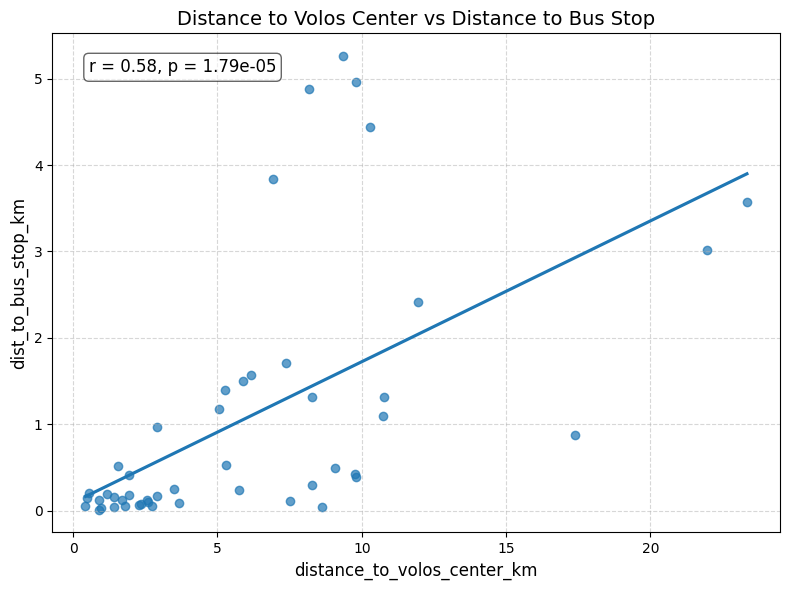
\includegraphics[height=5cm]{figures/scatter_center_transport.png}
        \caption{Scatter Plot: Distance from Center VS Distance from Transport Stops}
        \label{fig:scatter_center_transport}
    \end{minipage}
    \hfill
    \begin{minipage}[b]{0.47\textwidth}
        \centering
        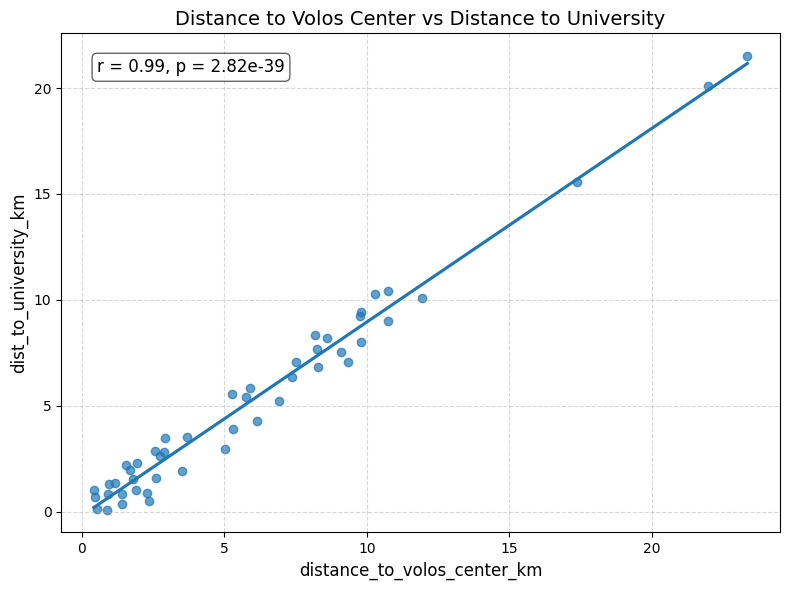
\includegraphics[height=5cm]{figures/scatter_center_uni.png}
        \caption{Scatter Plot: Distance from Center VS Distance from University}
        \label{fig:scatter_center_uni}
    \end{minipage}
\end{figure}

%==================================================
\subsection{EDA - Joined Dataset}

In the three previous sections we inspected and analyzed the 3 main datasets individually. To identify patterns among features originating from different datasets, we present below the analysis of the final joined dataset. It consists of 3882 entries and 42 total features \ref{tab:business_joined_columns}. Inspecting the missing data we see that the dataset is complete, except from the potential label columns ('Rating', 'Reviews', 'Description'), which are very sparse \ref{fig:heatmap_missing}. First, we attempted to relate the business category with several joined features. In order to use fewer categories to get the bigger picture, I grouped the NACE codes by division instead of class and found their mean values across some features. These graphs do not represent a cause and effect relationship between the NACE code and the feature, they just state the context by highlighting observed associations of the columns. 

\begin{figure}[h]
    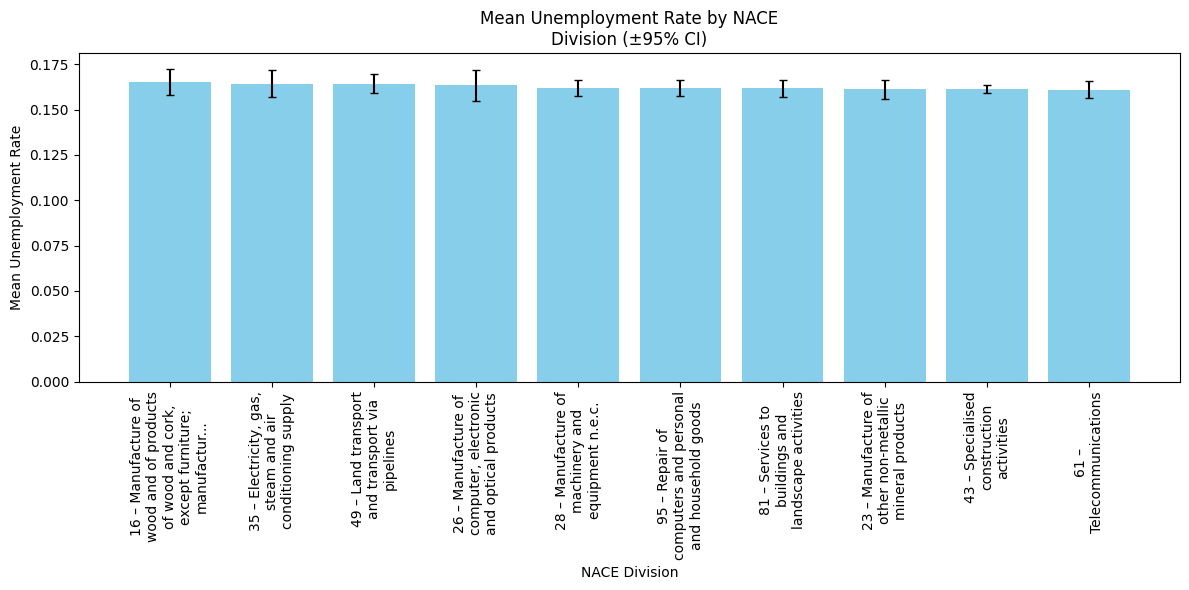
\includegraphics[scale=0.45]{figures/barchart_per_nace_unemployment.png}
    \centering
    \caption{Mean Unemployment per NACE Division Bar Chart}
    \label{fig:barchart_per_nace_unemployment}
\end{figure}

\begin{figure}[h]
    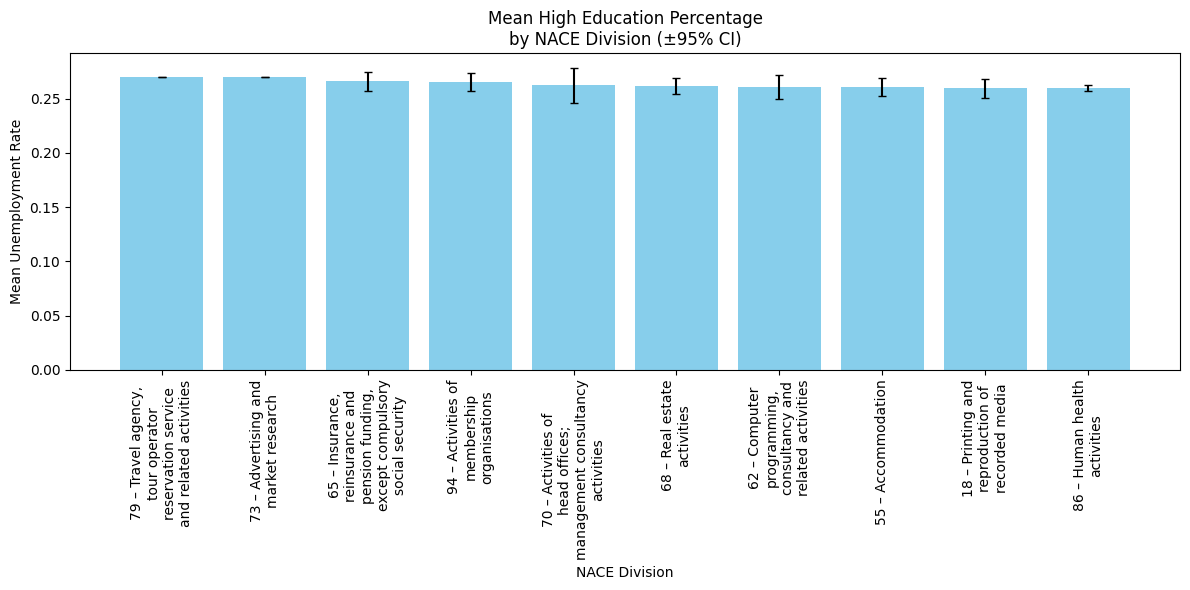
\includegraphics[scale=0.45]{figures/barchart_per_nace_highedu.png}
    \centering
    \caption{Mean High Education per NACE Division Bar Chart}
    \label{fig:barchart_per_nace_highedu}
\end{figure}

Regarding the unemployment rate, although the top values are similar, it is most dominant in the manufacture of wood, electricity and air conditioning supply, land transport, manufacture of computer and electronic products, and manufacture of machinery and equipment \ref{fig:barchart_per_nace_unemployment}. We also see a similar pattern when analyzing the high educational level per NACE division, with the highest values being in the following sections: travel agency, advertising, insurance, activities of membership organisations and management consultancy activities \ref{fig:barchart_per_nace_highedu}.


Despite the severe sparseness of ratings, they present a significant negative relationship with the unemployment rate. To acquire this I calculated the mean rating per municipal community and compared it with the unemployment rate. This indicates that areas that contain highly rated businesses tend to also have a lower unemployment rate value. As before, this only provides context for interpreting rating values that tend to occur alongside specific unemployment rates. I also tried to identify a connection between the rating and the distance from center, but there was no sufficient statistical evidence that supported this suspicion.

\begin{figure}[h]
    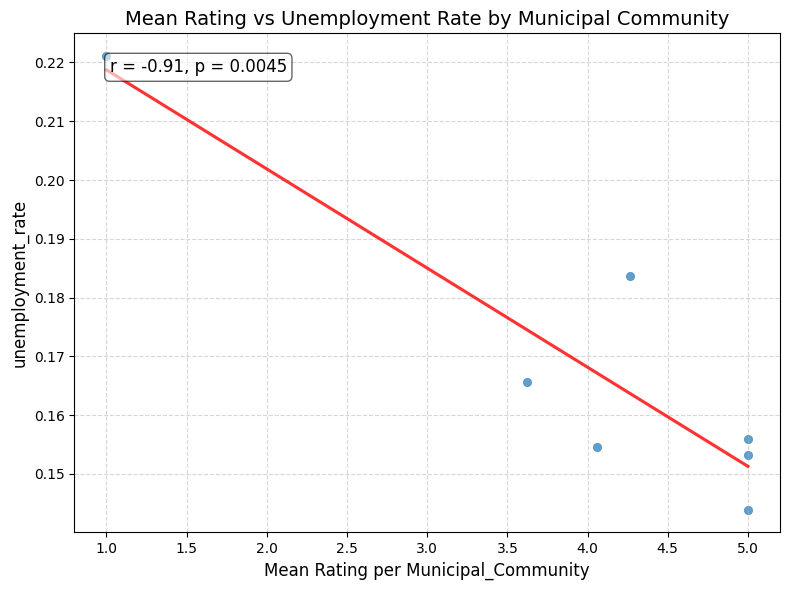
\includegraphics[scale=0.4]{figures/scatter_mean_rating_unemployment.png}
    \centering
    \caption{Scatter Plot: Mean Rating VS Unemployment Rate}
    \label{fig:scatter_mean_rating_unemployment}
\end{figure}




%==================================================
%==================================================
%==================================================
\section{Proxy Ground Truth Creation}
\label{sec:proxy}

In order to utilize machine learning for creating a recommendation system of optimal business locations, we need a criterion to rank the candidate areas for every category to use the top ones as labels. The intuitive approach would be to filter the entries for every NACE class, and use the rating average of every neighborhood to sort the best candidates. This is not feasible, however, due to the sparsity of the labels, so we were forced to create a proxy ground truth myself. 

Following principles of weak supervision and ensemble learning, three complementary approaches were implemented: supervised (learning from labeled instances), unsupervised (capturing latent data structure), and semi-supervised (expanding limited labels). To mitigate the bias of any single method and to also exploit the distinct aspect of the problem space that each approach captures, their outputs were ensembled into a unified ranking. While this does not provide the definitive ground truth, it establishes a consistent and interpretable proxy based on which the models can be trained and evaluated. For every approach, we implemented an attempt that only uses the neighborhood columns, and one that also includes the municipal community features. The two attempts were compared by measuring the amount of central suggestions they provide, and the best was kept.



%==================================================
%==================================================
\subsection{Supervised Learning Approach}

To address the lack of explicit labels, a supervised machine learning approach was first developed. The objective was to approximate the “success likelihood” of each location for a given business category (NACE code).


%==================================================
\subsubsection{Model Dataset Creation}

The worflow begins by creating the dataset that we aim to train the model on. The entries of the dataset consist of every possible (NACE class, Neighborhood) pair, therefore 306x48 = 14688 records. We join the entries with the features of its corresponding neighborhood, and in a second attempt, also with their corresponding municipal communities. The target column does not relate with the ratings, rather it is a new binary value, indicating the presence or absence of a business of this type in a given neighborhood \ref{fig:proxy_approach1}. The dataset presents a considerable class imbalance as only 11.58\% of the label values are 1.

\begin{figure}[h]
    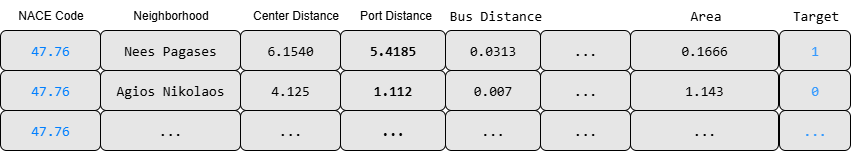
\includegraphics[scale=0.5]{figures/proxy_approach1.png}
    \centering
    \caption{ML Model Dataset Creation}
    \label{fig:proxy_approach1}
\end{figure}


%==================================================
\subsubsection{Top-10 Extraction}

The model used is a Random Forest with 100 decision trees. Prior to training, the input features were scaled to the range [0,1] using 'MinMaxScaler' to ensure comparability with other models in the pipeline. Once trained on the dataset, the model is inferenced to obtain prediction probabilities for every entry. These probability values are then used as ranking criteria for the neighborhoods within each NACE class, with the top 10 being selected as the proxy ground truths. Both attempts resulted in similar lists, but the second was chosen as it yielded a slightly higher percentage of central recommendations (81.48\% over 81.05\%). Although promising, this approach is limited by its implicit assumption that the presence of a business in a location implies a high probability of success, which is not always the case in real world scenarios.



%==================================================
\subsection{Unsupervised Learning Approach}

A second method that uses unsupervised learning was applied, with the goal of identifying the "ideal conditions" for each business category. Unlike the supervised method, this approach does not rely on labels but instead exploits the feature space structure.


%==================================================
\subsubsection{Clustering}

First, we filter the business entries for every NACE class and apply k-means clutering on them. The optimal value of the k parameter is determined by applying the eblow method. After the clusters are created, we determine the "ideal cluster" by comparing them based on the value of a "judge feature", in our case the ratings. Each cluster centroid represents the average profile of the businesses in that group, therefore the centroid of the ideal cluster is assumed to describe the "average ideal conditions" for the specific business type. 

%==================================================
\subsubsection{Top-10 Extraction}

Once the ideal cluster centroid is obtained, we can calculate its Euclidean distance into the same feature space with all the candidate neighborhoods and use it as the ranking criterion. The top 10 recommendations are the 10 neighborhoods closer to the centroid. In \ref{fig:cluster_distance} we see a 2D PCA projection of the high-dimensional feature space containing the candidates and their distance from the ideal cluster centroid for the NACE class 10.52. Although this time the recommendations do not occur solely based on the current business presence, the identification of the “ideal” cluster relies on a single judge feature, oversimplifying the multidimensional nature of business success. 

\begin{figure}[h]
    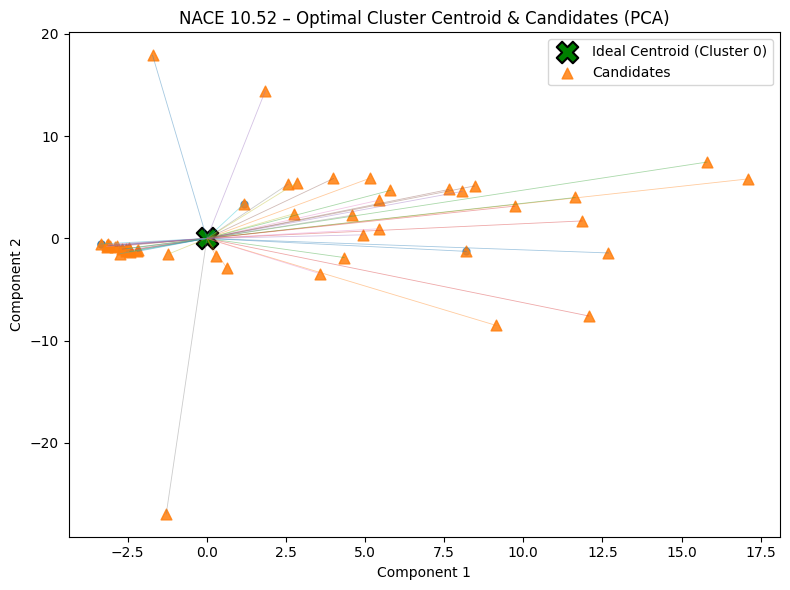
\includegraphics[scale=0.5]{figures/cluster_distance.png}
    \centering
    \caption{Ideal Cluster Centroid \& Candidates (2D PCA)}
    \label{fig:cluster_distance}
\end{figure}



%==================================================
%==================================================
\subsection{Semi-Supervised Learning Approach}

The third method adopted was a semi-supervised learning (SSL) technique, specifically self-training. SSL methods leverage both the limited labeled data and the large pool of unlabeled data by iteratively expanding the training set with pseudo-labels. 

%==================================================
\subsubsection{Self Training}

The model used is a Random Forest Regressor with 100 estimators. The process of self training start with training the initial model on the small set of labeled data (5.87\%). The trained model is then inferenced to produce labels (pseudo-labels) for the unlabeled entries. The pseudo-labels that are predicted "confidently" get integrated to the training set. The model is then re-trained on the updated training set, and the procedure repeats until either all the labels enter the set or no confident predictions occur \ref{fig:psudo_labels}. The confidence of the predictions is determined by comparing its variance to a predetermined threshold explicitly set at 0.1. 


%==================================================
\subsubsection{Top-10 Extraction}

After the ratings are enhanced, we can simply use the mean rating value of each neighborhood as the ranking mechanism to find the optimal locations for each business type. This time only neighborhood features were used since they provided a slightly higher percentage of central locations than the full feature approach. This method resulted to less than 10 recommendations for specific NACE classes since such business types did not exist within every neighborhood, so no rating was created. This is not a problem because the final proxy truths will be determined by combining all three approaches.

\begin{figure}[h]
    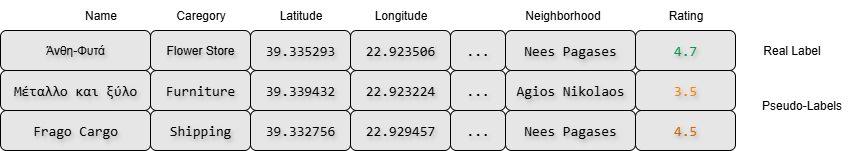
\includegraphics[scale=0.5]{figures/psudo-labels.png}
    \centering
    \caption{Real \& Pseudo Labels}
    \label{fig:psudo_labels}
\end{figure}


%==================================================
%==================================================
\subsection{Ensemble Method}

The techniques outlined in the previous sections capture and contribute an additional view of the problem, but they also suffer from multiple limitations. Following principles of ensemble learning, I combined the individual weaker predictions to obtain the final proxy ground truths. Below, we show a comparison of the individual results and then present their combined outcome.


%==================================================
\subsubsection{Comparison of Results}

Firstly, I compared the three individual proxy truth results to see if they agree or not. I computed the agreement count per NACE class, which essentially combines the total suggestions from all the sources along with their frequency. For example, NACE class 23.70 "cutting, shaping and finishing of stone" presented the following results: 3 votes for Agioi Anargiroi, 3 votes for Nea Ionia, 2 votes for Analipsi, and 1 vote for Epta Platania - Oksigono. In Figure \ref{fig:hist_unique_suggestions} we can see the histogram of the unique suggestions across all NACE classes. A total of 3 suggestions suggest a prefect agreement of the three methods, whereas with more suggestions their results tend to diverge. We see that the majority of different recommendations gathers at 4-6, implying a partial agreement between the techniques.


\begin{figure}[h]
    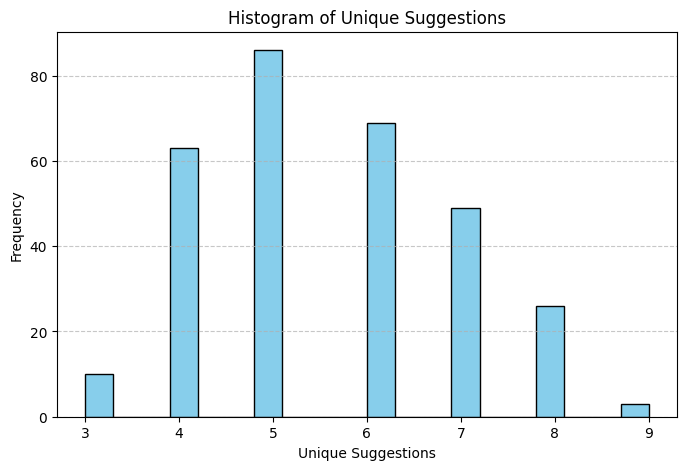
\includegraphics[scale=0.5]{figures/hist_unique_suggestions.png}
    \centering
    \caption{Unique Suggestions of all Methods Histogram}
    \label{fig:hist_unique_suggestions}
\end{figure}


Venn Diagrams can provide a more intuitive understanding of the similarity of the individual suggestions \ref{venn_diagrams}, but they only relate to a specific NACE class and not the wider picture as the histogram did. I also calculated the Jaccard similarity of every NACE class between the pairs of the three aproaches. Figure \ref{fig:barchart_jaccard_similarities} demonstrates the average Jaccard similarity across all NACE classes, and we see that the unsupervised and semi-supervised approach provide the most similar results. Spatial similarity within 1 kilometer was also measured, which measures how geographically close the suggestions are, even when they differ. This also showed that the supervised and unsupervised approaches were the most dissimilars, while the highest similarity was observed between the supervised and semi-supervised approaches.


\begin{figure}[h]
    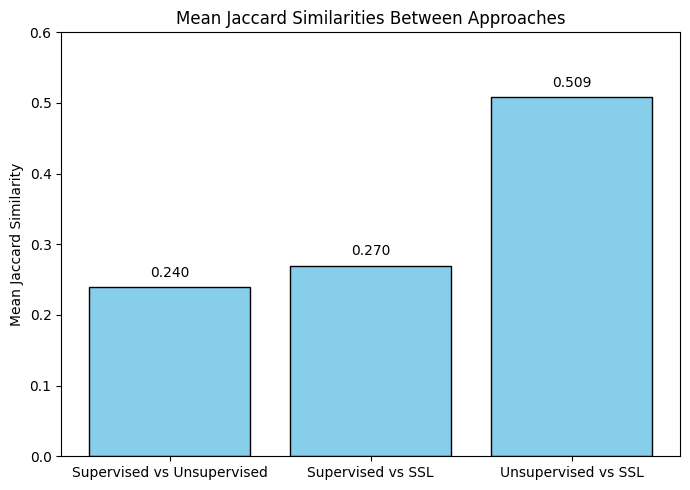
\includegraphics[scale=0.5]{figures/barchart_jacaard_similarities.png}
    \centering
    \caption{Mean Jaccard Similarities Bar Chart}
    \label{fig:barchart_jaccard_similarities}
\end{figure}




%==================================================
\subsubsection{Combination of Results}

To combine the outputs of multiple approaches into a single consensus ranking, a weighted rank aggregation procedure was implemented. Throughout this thesis we have assumed that the central locations tend to be favoured in general, therefore the weight that each approach gets assigned is based on the proportion of its recommendations that fell within the municipality of Volos after being normalized so they add up to 1. In table \ref{tab:weights} we see the central areas pectentage and the corresponding weight of each approach.

\begin{table}[ht!]
    \centering
    \begin{tabular}{|p{5cm}|p{5cm}|p{5cm}|}
        \hline
        \textbf{Approach} & \textbf{Central Suggestions Percentage} & \textbf{Weight} \\
        \hline
        Supervised & 81.48\% & $w_s = 0.3110$ \\ \hline
        Unsupervised & 93.79\% & $w_u = 0.3580$ \\ \hline
        Semi-supervised & 86.67\% & $w_{ss} = 0.3308$ \\ \hline
    \end{tabular}
    \caption{Central Areas Percentage and Weight of Approaches}
    \label{tab:weights}
\end{table}

In addition to method weights, the rank position of each suggested neighborhood was also weighted. Specifically, the following values were assigned: Top1 = 10, Top2 = 9, …, Top10 = 1. This happens to ensure that a candidate appearing higher in a method’s ranking contributed more strongly to the final consensus. In order to obtain the final neighborhood score, we simply perform the weighted sum of the method and rank position \ref{eq:score}: 

\begin{equation}
    \label{eq:score}
    score(N_i) = w_s \cdot top_{s,i} + w_u \cdot top_{u,i} + w_{ss} \cdot top_{ss,i}
\end{equation}

This cumulative score is the final ranking criterion. For every NACE class the candidates were sorted by their scores in descending order and the 10 highest were selected as the final proxy ground truth. In Table \ref{tab:top3} we provide some indicative examples of the final top 3 estimated locations for certain NACE classes.\\

\begin{table}[ht!]
    \centering
    \begin{tabular}{|M{1cm}|M{4cm}|M{3cm}|M{3cm}|M{3cm}|}
        \hline
        \textbf{NACE Class} & \textbf{NACE Description} & \textbf{Top 1} & \textbf{Top 2} & \textbf{Top 3} \\
        \hline
        1.13 & Growing of vegetables and melons, roots and tubers & Metamorfosi & Kato Lehonia & Palaia \\ \hline
        43.22 & Plumbing, heat and air conditioning installation & Agia Paraskeui & Nea Ionia & Agios Georgios \\ \hline
        68.32 & Management of real estate on a fee or contract basis & Agios Nikolaos & Agios Vasilios & Agios Konstantinos \\ \hline
        79.11 & Travel agency activities & Metamorfosi & Agios Konstantinos & Analipsi \\ \hline     
    \end{tabular}
    \caption{Final Top-3 Recommendations of NACE Classes}
    \label{tab:top3}
\end{table}




    \chapter{Methodology / System Implementation}
\label{chap4}


In this chapter we describe the modeling approaches that were used for the creation of the business location recommendation system. We begin by discussing the general motivation behind each method that led to their implementation and comparison, and then proceed to further analyze each in detail.


%==================================================
%==================================================
%==================================================
\section{Overview of Modeling Approaches}

Given the recommandation system we aim to implement, and the ambition to achieve this through the use of generative AI, two state-of-the-art approaches were suggested for the task, each with different strengths, limitations, and ways of utilizing the gathered data. An initial approach involves fine-tuning a Large Language Model (LLM) to specialize in predicting optimal locations while also providing a contextual and user-personalized response. An alternative approach that has emerged in recent years is the construction of a Retrieval-Augmented Generation (RAG) system. In this framework, the actual decision-making process takes place outside the LLM, which is instead used to generate the chatbot-like user output.

Both methodologies present different strengths, limitations and implementation details. In general, a fine-tuned LLM is expected to provide a faster inference that can generalize better on unseen prompts due to its wider knowledge as a pre-trained model. The RAG workflow ,on the other hand, supposedly reduces the hallucinations since its memory does not lie inside the LLM but it fetches data from databases at runtime, and can possibly lead to better personalization due to its more interpretable re-ranking ability. 




%==================================================
%==================================================
%==================================================
\section{Fine-tuned LLM}
\label{sec:fine_tuned_llm}

This section examines the approach of fine-tuning an LLM to specialize on the task of providing the three best locations to open a business. We will first analyze the motivation behind this method, then show the detailed process of creating the fine-tuning and inference datasets, and finally describe the fine-tuning attempts and their comparison based on their results on the inference dataset.


%==================================================
%==================================================
\subsection{Motivation}

Traditional recommendation systems, such as collaborative filtering, content-based filtering, and hybrid approaches, have long been prominent in the field of data science. Despite their indisputable effectiveness, limitations like the cold start problem (struggling when limited historical data is available) or the lack of the explainability of the recommendations have led to the gradual adoption of LLMs in the field. Although several attempts in general recommendation tasks (e.g. movies, products) have tested the suitability and success of LLMs, their application in spatial data and specifically business location recommendation is still very limited. In addition, the potential to provide contextual and personalized suggestions along with justification represents a novel yet promising approach that led to the idea of using LLMs for this problem. In the following paragraph, we show the creation of the essential datasets, the detailed fine-tuning, and the evaluation of the final model. 


%==================================================
%==================================================
\subsection{Fine-Tuning Dataset Creation}
\label{sec:fine_tune_dataset_creation}

This section describes analytically the construction of the fine-tuning dataset. This constitutes the core of the methodology, as the 
content and structure of the final model's outputs are learned directly based on its training data. 


%==================================================
\subsubsection{Synthetic NACE Categories}


The final goal is a model that responds to an every-day description of the business that the user is interested in, ("Where can I open a cafe in Volos?"), not one that specifically mentions its NACE class ("Where can I open a business of NACE class 56.3?"), since this encoding is too technical, or even unknown to the user. Therefore, training prompts should consist of such category descriptions and not the NACE classes themselves. In order to obtain such descriptions generative AI was used. Ιn particular, ChatGPT was produced 3 synthetic categories for each NACE class \ref{fig:synthetic_categories}. Each synthetic category will correspond to 1 entry on the fine-tuning dataset, resulting in 306x3 = 918 entries.

\begin{figure}[!htbp]
    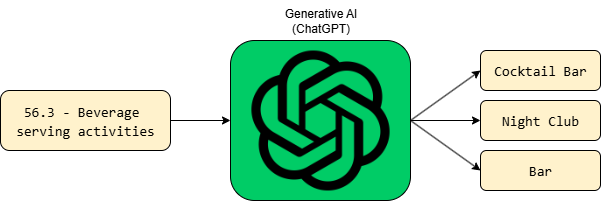
\includegraphics[scale=0.4]{figures/synthetic_categories.png}
    \centering
    \caption{Synthetic Categories Creation}
    \label{fig:synthetic_categories}
\end{figure}


%==================================================
\subsubsection{Feature Importance per NACE Class}

Looking forward, we aim to involve justification for every suggestion provided, as one of the primary motivations of using an LLM was explainability. Since the features describe various aspects of the suggestion (e.g. distance from city center, distance from main roads, area), we aim to use their values for the appropriateness of the recommendation. This requires deciding which features to include in the model's response, since using them all would generate unnecessarily long outputs. To make this decision, feature importance was found and used as a ranking criterion to select features from highest to lowest. The ranking was found individually for every NACE class, since it is assumed that feature importances change between different business types. To acquire the feature importances per NACE class, I used the 'shap' library.


\begin{figure}[h]
    \centering
    \begin{minipage}[b]{0.45\textwidth}
        \centering
        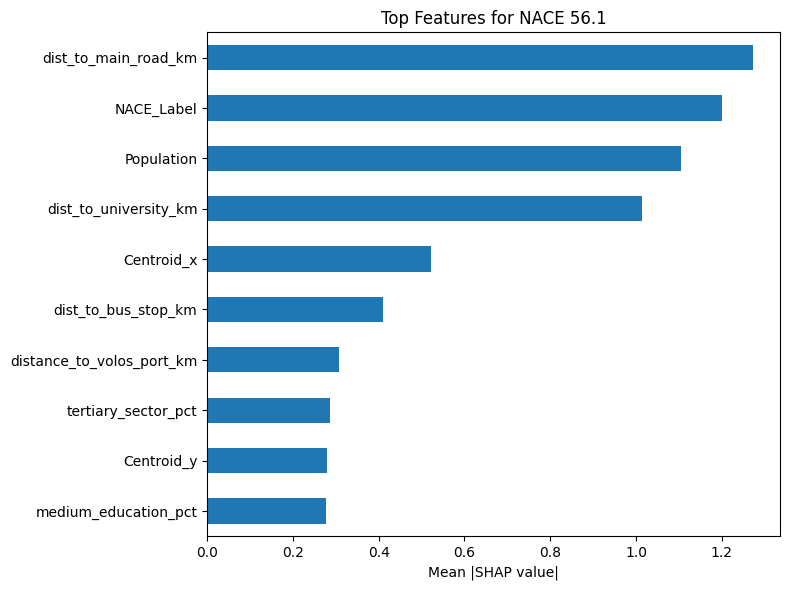
\includegraphics[height=5cm]{figures/shap_56_10.png}
        \caption{SHAP Values of NACE Class 56.10}
        \label{fig:shap_56_10}
    \end{minipage}
    \hfill
    \begin{minipage}[b]{0.45\textwidth}
        \centering
        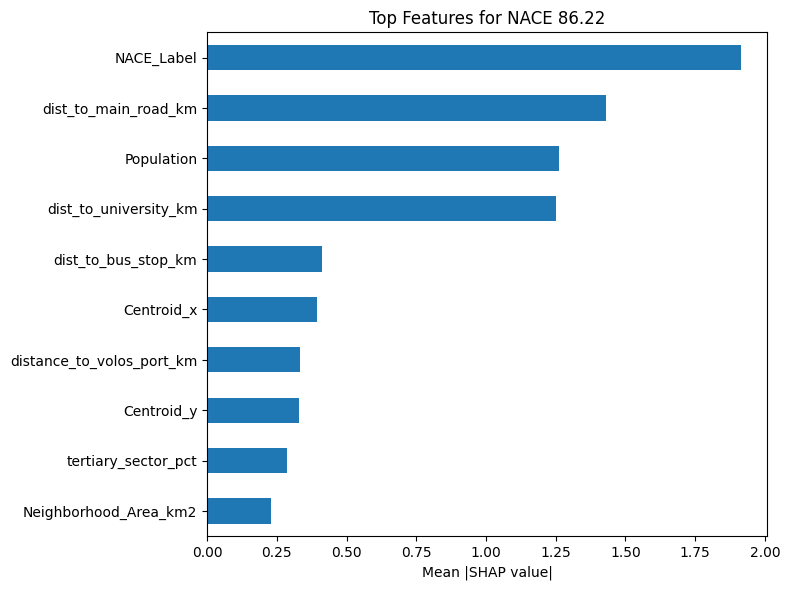
\includegraphics[height=5cm]{figures/shap_86_22.png}
        \caption{SHAP Values of NACE Class 86.22}
        \label{fig:shap_86_22}
    \end{minipage}
\end{figure}

An XGBoost machine learning model was trained on a dataset consistsing of all possible (NACE Class, Neighborhood) pairs, resulting in 306 x 48 = 14.688 entries. Each entry is joined with its corresponding neighborhood and municipal community features (apart from 'Neighborhood\_Greek', 'Geometry' and 'ΠΕΡΙΦΕΡΕΙΑΚΗ ΕΝΟΤΗΤΑ', 'ΔΗΜΟΣ', 'ΔΗΜΟΤΙΚΗ ΕΝΟΤΗΤΑ', 'ΔΗΜΟΤΙΚΗ ΚΟΙΝΟΤΗΤΑ ΕΛΛ' respectively). The label used is binary, indicating whether the specific neighborhood belongs to the top 3 recommendations for the corresponding NACE class. 

After model training, we extract its SHAP values to get insight on the feature importances. While the initial SHAP values refer to individual entries, they can be aggregated by averaging either across all NACE classes or even within each NACE class individually. In figures \ref{fig:shap_56_10}, \ref{fig:shap_86_22} we see the descending order of SHAP values for specific NACE classes, while in \ref{fig:shap_average} we see the mean feature importances across all columns. Beyond the NACE class itself, the largest average SHAP values are associated with population, distance to main roads, and distance to universities. The individual rankings will be the feature selection criterion when creating the training outputs.
 
\begin{figure}[!htbp]
    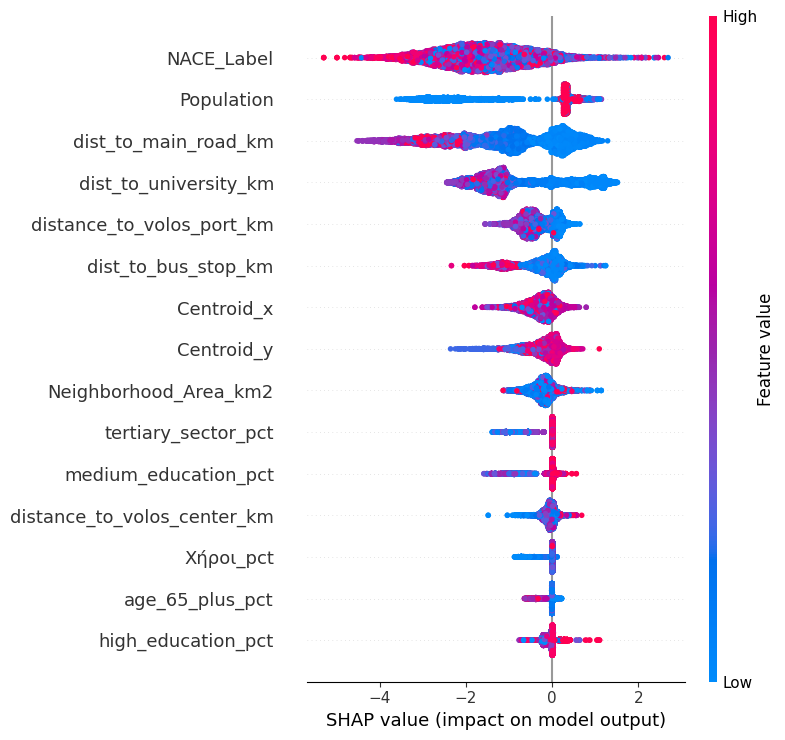
\includegraphics[scale=0.4]{figures/shap_average.png}
    \centering
    \caption{Average SHAP Values of all Features}
    \label{fig:shap_average}
\end{figure}


%==================================================
\subsubsection{Feature Statistics \& Feature Justification}
\label{sec:feature_justification}

The SHAP values displayed in the previous section described which features will be jutified, but did not explain how. To provide informative justifications for each feature, I calculated specific statistics per feature, namely the 25th, 50th, and 75th percentiles (q25, q50, q75). During feature justification, each feature value is compared with these percentiles to determine its corresponding interval. For every interval, 3 justification templates have been generated by ChatGPT, one of which is randomly selected to provide variation. From this point forward, we will refer to this process as "feature justification". Figure \ref{fig:feature_justification} visually demonstrates the different templates used based on the value and statistics.

\begin{figure}[!htbp]
    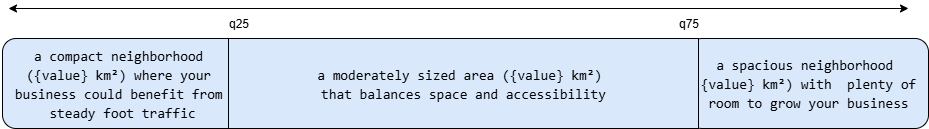
\includegraphics[scale=0.4]{figures/feature_justification.png}
    \centering
    \caption{Feature Justification for 'Neighborhood\_Area\_km2'}
    \label{fig:feature_justification}
\end{figure}


%==================================================
\subsubsection{Neighborhood Justification}
\label{sec:neigh_justification}

During the construction of training completions, we aim to provide explainable outputs which justify each recommendation. Building on the feature justification method described above, a complete reasoning about a neighborhood can be implemented by aggregating the justifications of several features. At this stage, it becomes essential to select certain features, as using them all would result in an overly large output. 

Six features were used to provide explainability to the output. Certain features, assumed to be consistently important, were treated as "fixed". Examples include neighborhood area, proximity to the city center, and distance from highways \ref{tab:fixed_features}. During neighborhood justification, 4 out of 7 fixed features are randomly selected and justified. The two remaining features were selected according to their SHAP values, specifically choosing the two most important features not included among the fixed ones. This combination of fixed features with SHAP importance balances consistency with variety of the training output.


%==================================================
\subsubsection{Prompt Construction}

The creation of training prompts is relatively straightforward. They are based on five synthetic templates generated by ChatGPT, each parametrised by the business category. When constructing the fine-tuning dataset the synthetic category is passed as input. Table \ref{tab:prompt_templates} displays the synthetic prompt templates. We generate one template per synthetic category, resulting in a total amount of 918.


\begin{table}[ht!]
    \centering
    \begin{tabular}{|M{10cm}|}
        \hline
        \textbf{Prompt Templates} \\ \hline
        "Where should I open a \textbf{\{category\}} in Volos?" \\ \hline
        "What is the best neighborhood in Volos for a \textbf{\{category\}}?" \\ \hline
        "I'm looking to start a \textbf{\{category\}}. Which area would be ideal in Volos?" \\ \hline
        "Suggest a location in Volos for a \textbf{\{category\}}." \\ \hline
        "Which place would you recommend for opening a \textbf{\{category\}} business in Volos?" \\ \hline
    \end{tabular}
    \caption{Synthetic Prompt Templates}
    \label{tab:prompt_templates}
\end{table}


%==================================================
\subsubsection{Completion Construction}
\label{sec:completion_construction}

The construction of training completions involves the justification mechanisms mentioned above. For every synthetic category, we extract the proxy top 3 recommendations of its corresponding NACE class as estimated in section \ref{sec:proxy}. The recommendations are transformed to explanatory text by applying the neighborhood justification method described previously \ref{sec:neigh_justification}, and combined to form the final completion. The workflow is shown intuitively in Figure \ref{fig:completion}.

\begin{figure}[h]
    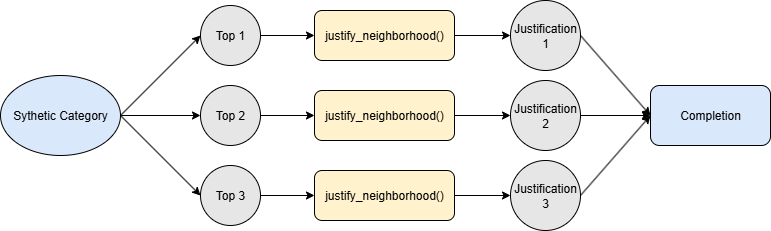
\includegraphics[scale=0.5]{figures/completion.png}
    \centering
    \caption{Completion Construction Workflow}
    \label{fig:completion}
\end{figure}


%==================================================
\subsubsection{Prompt-Completion Example}

To illustrate the fine-tuning dataset creation process, we present a prompt-completion pair generated for the synthetic category "greenhouse farming" that corresponds to the NACE class 1.13 in \ref{ex:prompt_completion_greenhouse}. The total prompt-completion pairs are 918 as mentioned before.

\begin{figure}[htbp]
  \centering
  \begin{tcolorbox}[myexample, title={Prompt-Completion Example}]
  \textbf{Prompt:} \emph{Where should I open a greenhouse farming business in Volos?}

  \vspace{0.5\baselineskip}
  \textbf{Completion:} \emph{Top neighborhoods for a Greenhouse farming business (NACE 1.13: Growing of vegetables and melons, roots and tubers) in Volos:}
  \begin{enumerate}
    \item \textbf{Metamorfosi} -- right near the university (0.14 km) --- great if you want to attract students or young professionals; a large local population, which can bring in steady foot traffic; a compact neighborhood (0.56 km$^{2}$) where your business could benefit from steady foot traffic; excellent central location (0.54 km), making your business easy to find and reach; accessible without being too exposed to street noise or congestion (0.16 km); fairly accessible by public transport (0.20 km), even if not right next to a bus stop.
    \item \textbf{Kato Lehonia} -- a balanced location (2.07 km$^{2}$) --- not too dense, not too open; a busy neighborhood with a strong base of potential customers nearby; close enough (8.62 km) to be convenient, while still offering some breathing room from downtown traffic; great access to main roads (0.01 km) --- easy for customers to reach you and for deliveries to run smoothly; not close to campus (8.21 km), which could work well for businesses focused on the neighborhood itself; excellent access to public transit (0.04 km), which can boost foot traffic to your business.
    \item \textbf{Agios Konstantinos} -- a moderately sized area (0.82 km$^{2}$) that balances space and accessibility; it's very close to the city center (1.41 km), which means great visibility and easy access; a reasonable distance from transit (0.16 km) --- close enough for most customers to reach you without much hassle; lots of people live in the area --- great for attracting walk-in customers; reasonably close to main roads (0.13 km), giving you decent accessibility without heavy traffic; a lively spot near the university (0.82 km) that could bring in a lot of student activity.
  \end{enumerate}
  \end{tcolorbox}
  \caption{Prompt-Completion Example}
  \label{ex:prompt_completion_greenhouse}
\end{figure}



%==================================================
%==================================================
\subsection{Inference Dataset Creation}
\label{sec:inference_dataset}

The construction of the inference dataset is similar to that of the training dataset, differing only in the synthetic categories used. Αll NACE classes were divided into two categories based on their frequency on the business entries dataset: classes that characterize at least 50 businesses were considered main classes, otherwise they are treated as secondary. The main classes are 53 and comprise almost 63.32\% of the total businesses. During the inference data creation only main classes are used. This is done to provide a more realistic model evaluation, as keeping only frequent business types results in an inference dataset representative of real-world examples. As before, 3 synthetic categories per class were generated, accounting for 3x53 = 159 total entries. The construction of the prompts and completions is identical to that described previously.


%==================================================
%==================================================
\subsection{Fine-Tuning Process}

After showing the construction of the training dataset, we can finally examine the fine-tuning process. Below, we mention details like computational recourses, the base model, and the fine-tuning techniques applied.


%==================================================
\subsubsection{Hardware \& Base Model}

The training was carried out on the high-performance computing cluster of University of Thessally, that utilizes an NVIDIA A100 GPU. Given our hardware capabilities, "mistralai/Mistral-7B-Instruct-v0.2" was chosen for its balance between strong instruction-following capabilities and computational efficiency. 

%==================================================
\subsubsection{Quantization \& QLoRA}

Fine-tuning was preformed using the QLoRA (Quantized Low-Rank Adaption) method, which combines quantization of the base model with integration of lightweight trainable adepter layers. In order to fit the 7 billion parameter within the available GPU memory, the base model weights were loaded in 4-bit NF4 quantization and kept frozen during training. Since these weights remain unchanged, LoRA adapters, specificlly 16-rank matrices, were inserted as trainable parameters. When the parameters of the model are printed, we get the values shown on Table \ref{tab:qlora}. The total parameters are displayed to be around 3.75 instead of 7 billion due to the compressed representation after quantization. In addition, the tiny percentage of trainable parameters demonstrates the effect of QLoRA adapters, resulting in a significantly more lightweight model with only 0.1813\% trainable weights.\\

\begin{table}[ht!]
    \centering
    \begin{tabular}{|p{5cm}|p{5cm}|}
        \hline
        Total Parameters & 3.758.895.104 \\
        \hline
        Trainable parameters & 6.815.744 \\ \hline
        Trainable \% & 0.1813\% \\ \hline
    \end{tabular}
    \caption{Model Parameters after QLoRA}
    \label{tab:qlora}
\end{table}


%==================================================
\subsubsection{Tokenization \& Label Masking}

Before performing the model fine-tuning, each prompt-completion example was converted to compatible formatting for the Mistral-Instruct tokenizer, using the template \ref{eq:inst_format}. The formatted string is then tokenized using a fixed length, either by truncation or padding, set to 512 after determining that 95\% of the formatted strings result in 462 or less tokens.

\begin{equation}
    \texttt{<s>[INST] {prompt} [/INST] {completion} </s>}
    \label{eq:inst_format}
\end{equation}

To ensure the model learns to predict only the completion and not the prompt, the labels of the instruction's tokens are masked out by setting their value to -100 so they get ignored when computing the crossentropy loss function.

%==================================================
\subsubsection{Training Configuration}

As we previously mentioned, 4-bit NF4 quantization was used along with QLoRA adapters of rank 16. The scaling factor, which determines the influence of the adapters, is set to 64, which is a balanced, standard choice. During the training we used an effective batch size per device of 2 and a gradient accumulation of 4, resulting in a total effective batch size of 8. The learning rate was set to 2e-5. The complete training configurating is displayed on table \ref{tab:finetune_config}. Regarding the number of epochs, three attempts were made with 3, 5, and 8 epochs respectively. The results will be further explored in chapter 5.


%==================================================
%==================================================
\subsection{Fine-Tuned LLM Workflow Summary}


So far we described the complete fine-tuning process. After training the model, its workflow is relatively straight forward. The LLM is simply fed a text input, and produces the predicted output. We showcase the workflow here to compare it later with the RAG pipeline, whose workflow is a bit more complex. Figure \ref{fig:workflow_ft} provides an intuitive visualization of the system.

\begin{figure}[h]
    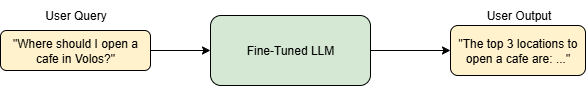
\includegraphics[scale=0.5]{figures/workflow_ft.png}
    \centering
    \caption{Fine-Tuned LLM Workflow}
    \label{fig:workflow_ft}
\end{figure}



%==================================================
%==================================================
\subsection{Inference Process}

After performing model fine-tuning, the resulting LLM is used on the inference dataset described in \ref{sec:inference_dataset}. This process was also run on the NVIDIA A100 GPU of University of Thessally. To ensure computational efficiency, inference was performed in batches of size 8. The outputs are stored, as they will be used later to evaluate the model performance by comparing them to the completions created in section \ref{sec:completion_construction}.




%==================================================
%==================================================
%==================================================
\section{RAG with Re-Ranking Pipeline}
\label{sec:rag}

This section explores the second state-of-the-art method that was implemented, a Retrieval-Augmented Generation workflow. First, we examine the motivation for exploring this method despite having already implemented the LLM fine-tuning approach. Followingly, we will show the creation of neighborhood descriptions that will be utilized in the framework. Finally, we will present the complete RAG pipeline, including the selected embedder, its application, and the integration with a generative LLM to produce the final output.



%==================================================
%==================================================
\subsection{Motivation}

While fine-tuning an LLM as described in section \ref{sec:fine_tuned_llm} indeed utilizes generative AI in an innovative way to address the problem of business location recommendation, it presents several important constraints. Adding proxy truths for new NACE classes or modifying existing ones requires re-running the entire fine-tuning process, which is both time consuming and computationally expensive. The desire to avoid this makes the approach static. Moreover, the justifications may not always include valid numbers, since LLMs are prone to hallucinations. Furthermore, since the model essentially learns to predict three static recommendations per NACE class, personalization may be difficult if users have specific preferences. A Retrieval-
Augmented Generation can potentially handle these problems because its memory is not stored inside the LLM and can be updated without extensive training In addition, the system outside of the LLM can adjust the final recommendations based on specific user desires, potentially allowing for better personalization.



%==================================================
%==================================================
\subsection{Neighborhood Description Creation}
\label{sec:neigh_desc}

Looking forward, we aim to compare the initial user query with the candidate locations to recommend the appropriate ones. Since the query is a text input which can be embedded into a dense vector representation, the first step was to create a text description per neighborhood that will later be also embedded and compared with the user query. The creation of descriptions is based on the core concepts used in the fine-tuning dataset construction \ref{sec:fine_tune_dataset_creation}, specifically the neighborhood justification method which essentially integrates multiple feature justifications.


%==================================================
\subsubsection{Feature Statistics \& Feature Justification}

This process is identical to the feature justification workflow explained in section \ref{sec:feature_justification}. The same statistic values are calculated for every feature, resulting in a specific text justification depending on the comparison of the individual feature's value in comparison with its percentiles. Once more, we randomly select one out of three templates per precentile interval for variety.


%==================================================

\begin{figure}[htbp]
  \centering
  \begin{tcolorbox}[myexample, title={Neighborhood Description}]
  \vspace{0.5\baselineskip}
  \textbf{Agios Nikolaos:} \emph{Neighborhood description:\\}
    A cozy location (0.35 km$^{2}$) that might work well for storefronts or quick-service ideas; it's very close to the city center (0.90 km), which means great visibility and easy access; very close to the port (0.53 km), which makes transport and logistics a lot easier; great access to main roads (0.00 km) — easy for customers to reach you and for deliveries to run smoothly; excellent access to public transit (0.01 km), which can boost foot traffic to your business; close to campus (0.09 km), which means steady foot traffic from a younger, educated crowd; a busy neighborhood with a strong base of potential customers nearby; a neighborhood with many single adults (40\%) — ideal for modern, fast-moving business models; fewer married residents (46\%), which could favor services tailored to individuals or younger adults; not a heavily elderly area (8\%), which could favor modern, fast-paced, or tech-forward businesses.
  \end{tcolorbox}
  \caption{Description for Agios Nikolaos}
  \label{fig:description_agiosnikolaos}
\end{figure}

\subsubsection{Neighborhood Description}
\label{sec:neigh_description}

The generation of descriptions is very similar to the construction of neighborhood justifications described previously \ref{sec:neigh_justification}, with some minor modifications. The major difference is that, in this case, producing large text is not a problem. While previously these justifications were used as LLM outputs and therefore had to be constrained, in this case, we aim to embed them. Hence, including as much information as possible about the neighborhood is not only acceptable but beneficial.

In more detail, the same fixed features are used \ref{tab:fixed_features}, but a justification is provided for all of them rather than only a subset. The total number of features used is also increased, resulting in a larger amount of secondary features as well. In \ref{fig:description_agiosnikolaos} we provide an indicative example of a neighborhood description.




%==================================================
%==================================================
\subsection{Embedding and Retrieval Process}

The RAG pipeline uses an embedder model that transforms text descriptions into high-dimensional dense vector representations. This enables similarity search between user queries and neighborhood descriptions. 



%==================================================
\subsubsection{Embedder Model}

To perform the embeddings, we selected the model "BAAI/bge-large-en-v1.5". This is a BERT-style transformer encoder with about 335 million parameters, optimized for semantic similarity search and RAG pipelines. It uses a vocabulary size of 30.522 tokens, 24 transformer layers, and the generated embeddings are of dimension 1024.


%==================================================
\subsubsection{Embedding NACE Descriptions}
\label{sec:embedding_nace}

As we will explain later, after acquiring the user query, the first step is to determine the NACE class of the business the user wants to open. This will be done by performing a vector similarity search between the query embedding and all NACE class descriptions. To avoid embedding all NACE descriptions in real time, we precompute the vector representations once and store them, allowing them to be retrieved during runtime. They are stored in the JSON file 'nace\_descriptions\_embeddings.json'.


%==================================================
\subsubsection{Embedding Neighborhood Descriptions}
\label{sec:embedding_neigh}

After determining the NACE code, we could simply use its corresponding proxy truths to provide the recommendations. In order to allow better personalization, however, we utilize a re-ranking method that initially fetches the top 10 suggestions, and re-ranks them based on vector similarity between them and the user query. This requires embedding the neighborhood descriptions created in section \ref{sec:neigh_description}. As we previously did with the NACE descriptions, the embedding generation of neighborhood descriptions is performed once, and stored in the JSON file 'neighborhoods\_descriptions\_embeddings.json'.


%==================================================


\subsubsection{Retrieval Process Output}

The re-ranking process results in an updated sorted list of top 10 recommendations. Since the structure of the final output should consist of three suggestions, we simply select the three most similar neighborhoods. Figure \ref{fig:retrieval} demonstrates the complete retrieval process as described in the previous sections.



\begin{figure}[!htbp]
    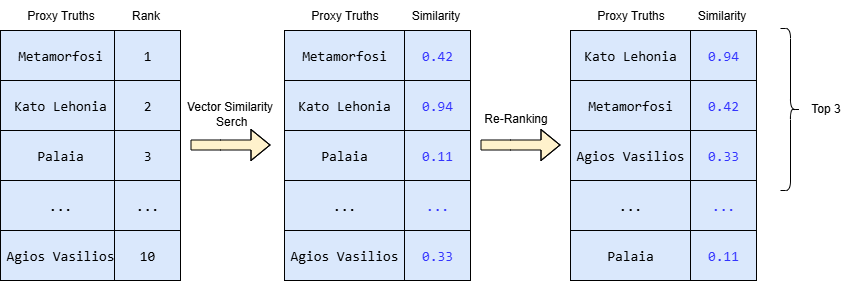
\includegraphics[scale=0.5]{figures/retrieval.png}
    \centering
    \caption{Retrieval Process}
    \label{fig:retrieval}
\end{figure}


%==================================================
%==================================================
\subsection{LLM Integration}

The retrieval process extracts the final suggestions that are intended to be presented to the user. In order to present them in a coherent, user-friendly recommendation, we utilize an LLM that receives the raw recommendations and descriptions and produces the final output message. In contrast with the fine-tuned LLM approach, in this case the LLM does not decide the actual recommendations, it acts only as the output generator.



%==================================================
\subsubsection{Selected LLM}

For user output generation, Llama 3 (8 billion parameters) was used. The model is run locally via Ollama, and thus is loaded in 4-bit quantization to ensure compatibility with the local hardware. It supports a context length of 8192 tokens and embedding dimensionality of 4096. During retrieval-augmented generation, the model is simply fed a specifically structured input and inferred to obtain the user output.


%==================================================
\subsubsection{LLM Prompt Construction \& Final Output}

To ensure clarity and user-friendly outputs, a structured template was constructed to guide the final output of the LLM. The template initially specifies the user query with the extracted NACE class and its description. Next, it mentions the three recommendations with their descriptions, and finishes by providing certain explicit output instructions. Figure \ref{fig:llm_prompt} shows an indicative example of the LLM prompt constructed to provide recommendations to the query "Where in Volos should I start a bakery business?". The descriptions are incomplete to fit the whole prompt. After the LLM prompt is constructed, we simply feed it to the model and infer it to acquire the final output. This is the final response that the user receives from our system.
 

\begin{figure}[!htbp]
  \centering
  \begin{tcolorbox}[myexample, title={LLM Prompt Example}]
  \vspace{0.5\baselineskip}
    The user wants to open a business of type: "Where in Volos should I start a bakery business?"\\
    **NACE Code: 46.36 — Wholesale of sugar and chocolate and sugar confectionery**\\
    Based on data analysis, here are the top 3 recommended neighborhoods in Volos:\\
    
    **Hiliadou** – a balanced location (1.03 km²) — not too dense, not too open, you'll be right near the heart of Volos (1.17 km) — convenient for both customers and deliveries, ...\\
    
    **Karagats** – a cozy location (0.67 km²) that might work well for storefronts or quick-service ideas, it's very close to the city center (0.98 km), which means great visibility and easy access, ...\\
    
    **Metamorfosi** – a cozy location (0.56 km²) that might work well for storefronts or quick-service ideas, you'll be right near the heart of Volos (0.54 km) — convenient for both customers and deliveries, ...\\
    
    Please present the 3 neighborhoods in a numbered list format like this:\\
    1. Neighborhood Name: Summary of strengths...\\
    2. Neighborhood Name: Summary of strengths...\\
    3. Neighborhood Name: Summary of strengths...\\
    Each point should be 2–4 sentences long, clearly explaining why the neighborhood is a good fit for the business. Avoid ranking or comparisons — describe each one positively and independently.
  \end{tcolorbox}
  \caption{LLM Prompt Example}
  \label{fig:llm_prompt}
\end{figure}



%==================================================
%==================================================
\subsection{RAG Pipeline Workflow Summary}

In the previous sections we examined the individual parts of the RAG framework. Here, we present a summary of the complete workflow. The system first receives the user query that asks about a specific type of business. Using the embedder, the entry is converted into a high-dimensional vector in real time. We find the corresponding NACE class of the business type by calculating the similarity between the query embedding, and the embedding of all NACE descriptions, which are pre-computed and stored locally. Next, we fetch the top 10 proxy recommendations of the NACE class, and apply vector semantic similarity once more, this time between the query and the neighborhood embeddings which are also available locally. The similarities are used as the re-ranking criterion to acquire personalized suggestions.   

The three neighborhoods with higher similarity scores are the final recommendations. In order to return a cohesive and context-aware message to the user, we pass the recommendations and their descriptions to a specifically structured template, and feed this to the Llamma 3 LLM to produce the final output. Figure \ref{fig:rag_workflow} visually shows the complete pipeline.


\begin{figure}[h]
    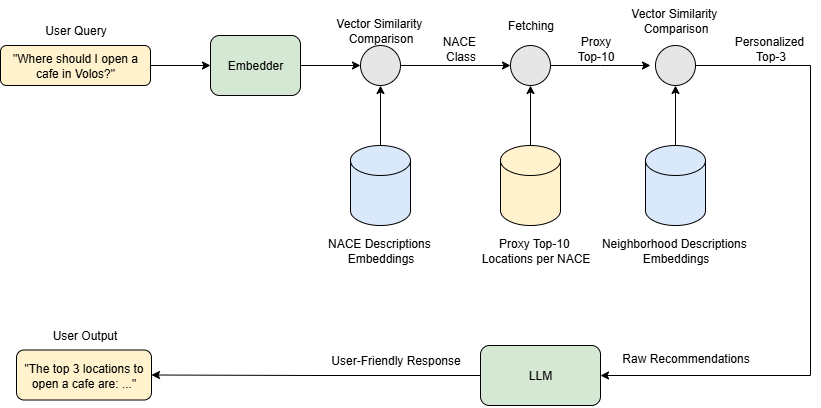
\includegraphics[scale=0.5]{figures/rag_workflow.png}
    \centering
    \caption{RAG Pipeline}
    \label{fig:rag_workflow}
\end{figure}


%==================================================
%==================================================
\subsection{Inference Process}
\label{sec:inf_rag}

After implemention the complete RAG pipeline, it is used on the inference dataset described in \ref{sec:inference_dataset}. In contrast to the fine-tuned LLM inference, this process is run locally since the loaded embedder is of reasonable size (355 million parameters) and the loaded LLM is quantized. The outputs are stored, as they will be used later to evaluate the pipeline performance by comparing them to the completions created in section \ref{sec:completion_construction}.



%==================================================
%==================================================
%==================================================
\section{Chatbot Interface}

The previous sections \ref{sec:fine_tuned_llm} and \ref{sec:rag} essentially describe the process of constructing frameworks that receive a text input and return a text output. In order to create a user-friendly application we create a chatbot-like interface. This section describes the frontend and backend development of the application, highlighting the mechanism that transforms simple LLMs into chatbots by memorizing the conversation.

%==================================================
%==================================================
\subsection{Frontend Development}

The frontend construction regards the form of the final user interface. Below we describe details of the fontend implementation. We start by mentioning why we chose the 'Streamlit' library, then showcase the interface design, and finally explain how the chat memory is stored in the frontend.


%==================================================
\subsubsection{Streamlit Framework}

Streamlit is an open-source Python framework designed to develop application frontends in a simple and efficient manner. Unlike traditional web frameworks, like React or Django, which require extensive knowledge of front-end technologies, Streamlit supports direct implementation in Pythn scripts. This makes it a great option for deploying machine learning models, where our primary goal is to provide a simple user interface rather than create a complex application. In the context of this thesis, Streamlit was utilized to implement the chatbot interface, as it provides a built-in session management and a simple layout system that can be easily integrated with a Python backend. \\



%==================================================
\begin{figure}[h]
    \centering
    \fbox{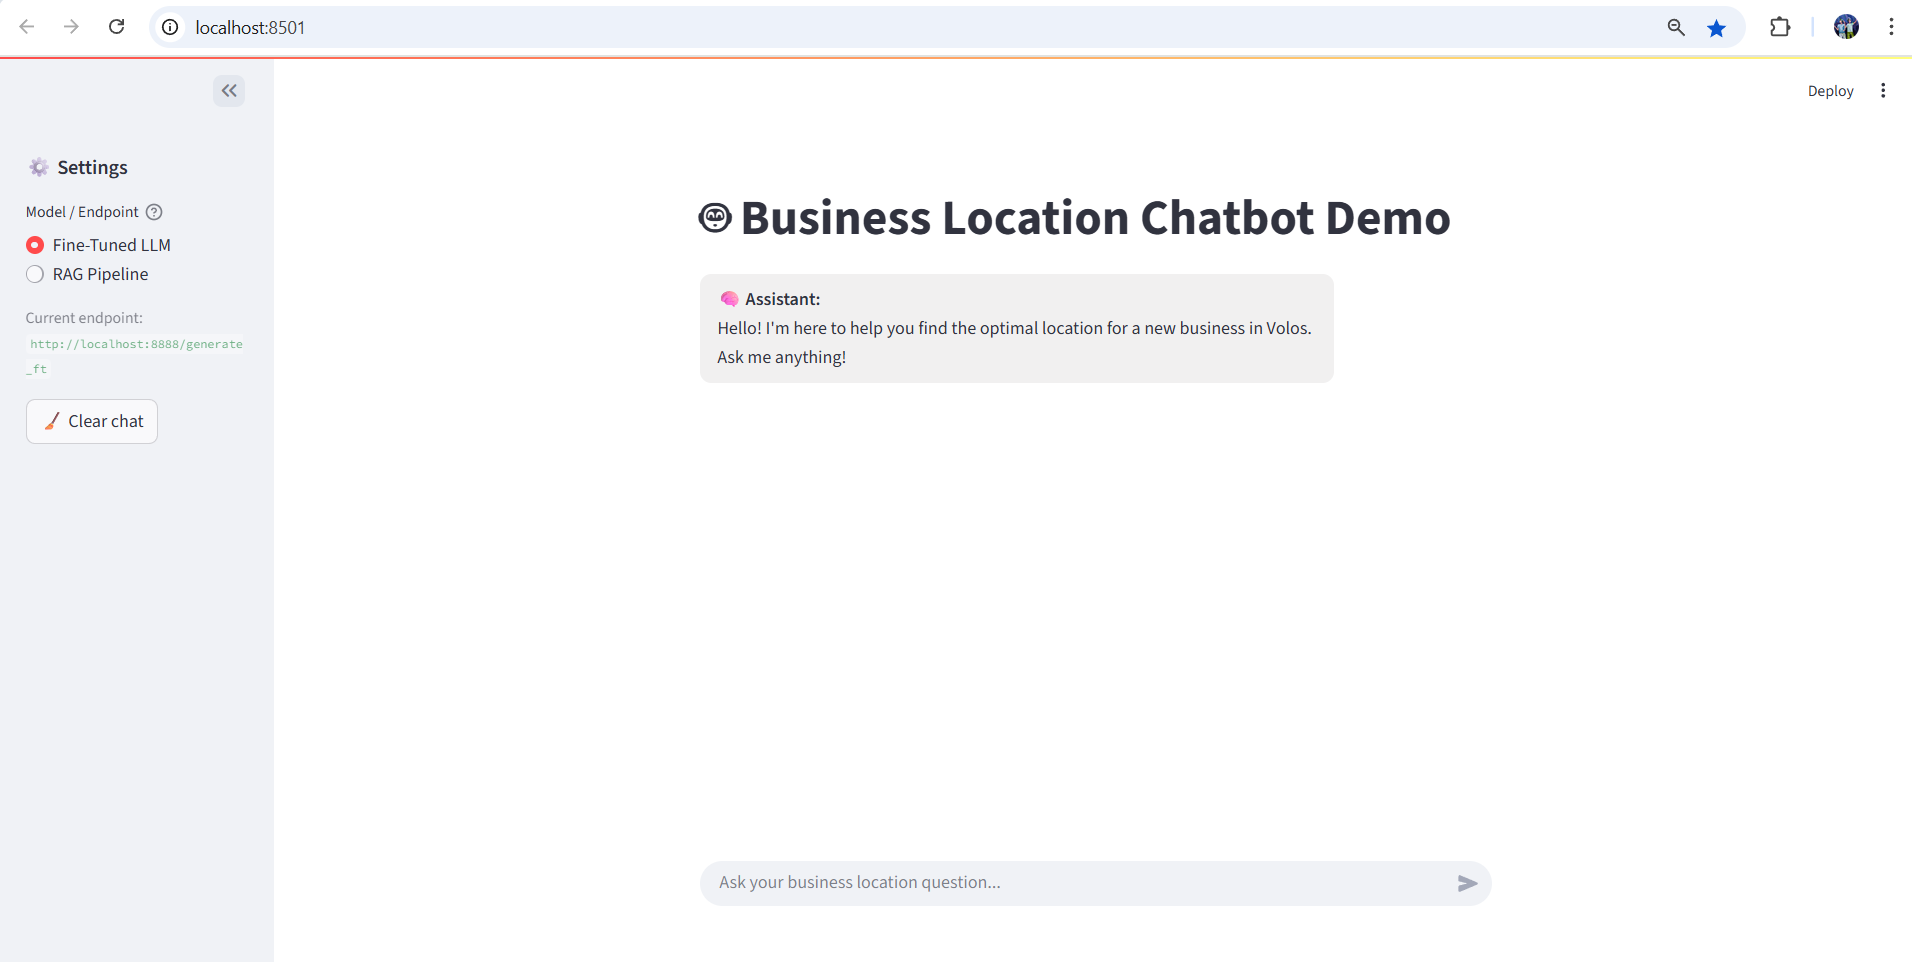
\includegraphics[scale=0.35]{figures/interface.png}}
    \caption{User Interface Design}
    \label{fig:interface}
\end{figure}


\subsubsection{User Interface Design}

The application design aims to mirror a state-of-the-art interface that provides a user-friendly experience. The page is initialized with the title "Business Location Chatbot Demo" and a greeting message from the AI assistant. At the bottom of the screen, an input box expects the input of the user. To improve readability, the conversation messages were designed with simple HTML and CSS embedded in Streamlit \ref{lst:render_user}, \ref{lst:render_assistant}. The assistant messages are shown in gray and aligned to the left, with the title "Assistant:". In contrast, the user messages appear in blue color, aligned to the right, and using the title  "You:". The interface dynamically updates after every new message. To ensure a continuous flow of conversation, when a user query is submitted, a spinner animation is displayed until the request is completed, and the response is displayed as well. The interface also contains a sidebar, that allows the user to select the backend system used, which we further explain in section \ref{sec:backend_development}. Figure \ref{fig:interface} shows an indicative screenshot of the application design, along with the greeting message.


%==================================================
\subsubsection{Session \& Memory Management}

During Streamlit sessions, the Python script is re-executed on every user interaction. In order to save the conversation history, we use the 'st.session\_state' object, which contains messages within the same session. The messages are stored as JSON objects, with fields: 'role', which identifies wether this is a user or assistant message, and 'content', which contains the actual message. At the beginning of a new session, the session state is initialized only with the greeting message. Every new message, whether from the user or the assistant, is integrated into the state. This mechanism essentially stores the conversation memory in the frontend. The complete history is then forwarded to the backend and processed from there, as we will analyze below.



%==================================================
%==================================================
\subsection{Backend Development}
\label{sec:backend_development}

The backend acts as the bridge between the user interface and the AI models. It is responsible for handling requests from the frontend, producing the output by using the systems we implemented, and returning it as a response. Below, we explain the framework selected to build the backend and the endpoint functions for each method. It is important to highlight that, while the inference of the RAG framework ran locally \ref{sec:inf_rag}, in order to use one server for the application, we run both approaches remotely on the computational cluster of University of Thessally.


%==================================================
\subsubsection{FastAPI Framework}

FastAPI is a modern Python framework, specifically designed for building APIs efficiently. Compared to traditional frameworks such as Flask or Django, FastAPI is lightweight and more simple. One of its main advantages is the support of asynchronous requests, which makes it suitable for long-running processes. This makes it ideal for our case, as querying a language model can be modeled in this framework.



%==================================================
\subsubsection{Fine-Tuned LLM Pipeline}
\label{sec:backend_ft}

The fine-tuned LLM approach is wrapped in the FastAPI endpoint '/generate'. When the Python script starts running, we load the LLM ('mistralai/Mistral-7B-Instruct-v0.2') in 4-bit quantization and attach the LoRA adapters created during fine-tuning on top of it. Once the model is active, it listens for user queries. The process is almost identical to the simple inference of the fine-tuned LLM system, with minor changes. In order to transform a simple LLM module into a chatbot, we simply have to modify the system input. 

\begin{figure}[h]
    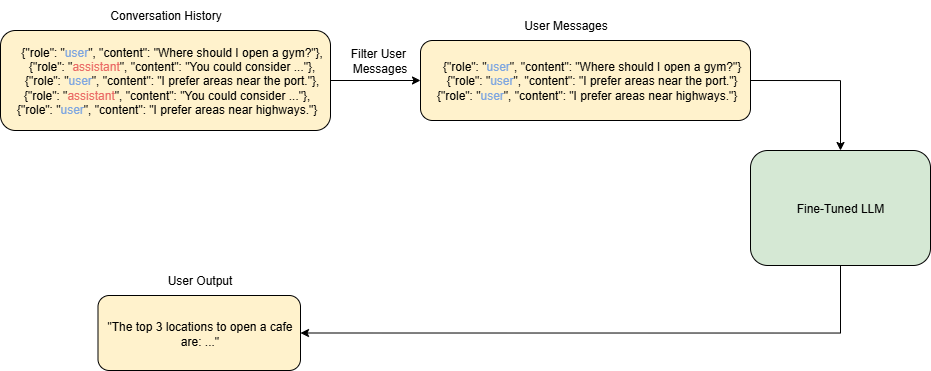
\includegraphics[scale=0.35]{figures/backend_ft.png}
    \centering
    \caption{Backend Fine-Tuned LLM Pipeline}
    \label{fig:backend_ft}
\end{figure}

As described previously, when a user query is received, a request is made from the frontend to the backend, containing the complete conversation history. The fine-tuned LLM extracts only the user messages and concatenates them to create the complete input. We treat the first user message as the ’intent’, since we assume that it contains the desired business type. The rest of them are treated as ’constraints’, based on the assumption that the follow-up messages specify preferences of the user. By combining the intent and constraints we create a prompt that always contains the desired NACE class, and also is up to date with every user specification. Figure \ref{fig:backend_ft} demonstrates this workflow.



%==================================================
\subsubsection{Retrieval-Augmented Generation Pipeline}
\label{sec:backend_rag}

The Retrieval-Augmented Generation pipeline is wrapped in the FastAPI endpoint '/generate\_rag'. In the beginning of the Python script, we load the embedder model ('BAAI/bge-large-en-v1.5') with its tokenizer, and we fetch the pre-computed embeddings of the NACE and neighborhoods descriptions described in section \ref{sec:embedding_nace}. The process again mirrors the inference of the system.

\begin{figure}[h]
    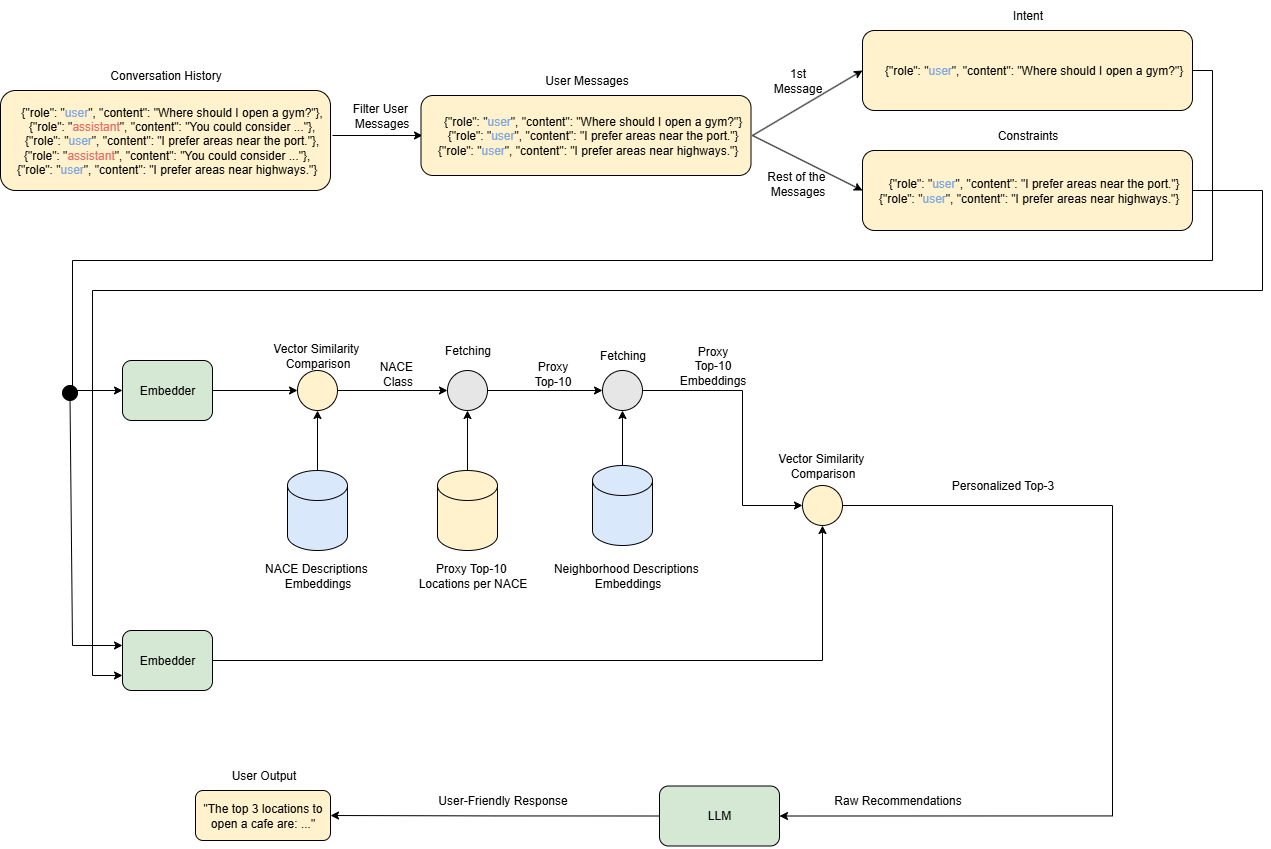
\includegraphics[scale=0.35]{figures/backend_rag.png}
    \centering
    \caption{Backend RAG Pipeline}
    \label{fig:backend_rag}
\end{figure}

The RAG system also extracts only user messages. We use just the intent to specify the NACE class, as the constraints should not affect the type of the business, only the actual recommendations. During the re-ranking, we embed the intent along with the constraints to fetch the final suggestions. Figure \ref{fig:backend_rag} shows the workflow visually.




%==================================================
%==================================================
\subsection{Frontend-Backend Communication}

The frontend communicates with the backend using synchronous HTTP POST requests to FastAPI endpoints. FastAPI provides a lightweight and JSON-friendly communication protocol that can easily be integrated with the Streamlit interface. Two main endpoints are available: '/generate', for deploying the fine-tuned LLM approach described in section \ref{sec:backend_ft}, and '/generate\_rag' for the RAG system pipeline explained in section \ref{sec:backend_rag}. The request messages send a JSON payload that contains the complete conversation history, together with a fixed system prompt that guides the output of the selected system \ref{fig:system_prompt}.\\


\begin{center}
    \fbox{\parbox{0.8\linewidth}{
    \textit{"You are a helpful assistant that suggests optimal business locations in Greece based on demographics and area characteristics."}
    }}
    \captionof{figure}{System Prompt for LLM Guidance}
    \label{fig:system_prompt}
\end{center}

The complete communication process can be summarized as follows: The frontend receives the user input, integrates it to the conversation, forwards the updated conversation history to the backend, which processes it, generates a response, and returns it. This approach ensures a clear and modular role for each side of the system. Figure \ref{fig:communication} intuitively displays the communication workflow between the frontend and the backend.\\

\begin{figure}[h]
    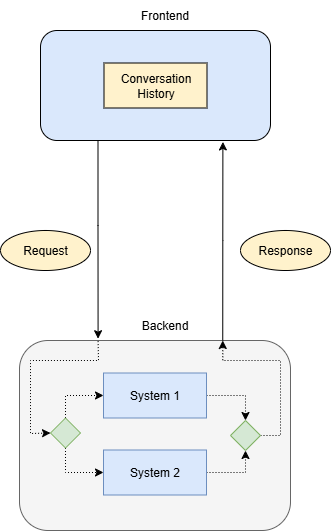
\includegraphics[scale=0.35]{figures/communication.png}
    \centering
    \caption{Frontent-Backend Communication}
    \label{fig:communication}
\end{figure}



%==================================================
%==================================================
\subsection{Chatbot Demo}

The previous sections described the process of transforming an LLM-based system, which simply receives a text input to a text output, to a chatbot application, with memory for the conversation history and a complete fontend-backend communication system. Below, we present an example of a conversation for every approach to demonstrate the results.


%==================================================
\subsubsection{Fine-Tuned LLM Approach}

Figure \ref{fig:chatbot_inf_ft} shows an example of a conversation using the fine-tuned LLM. We see that the structure of the output resembles the training data, which is expected, since the LLM learns to follow this specific pattern. In this case, we see a mistaken prediction, since the constraint about areas close to the ports actually results in a number 1 option, whose port distance is larger than options 2 and 3.

\begin{figure}[h!]
    \centering
    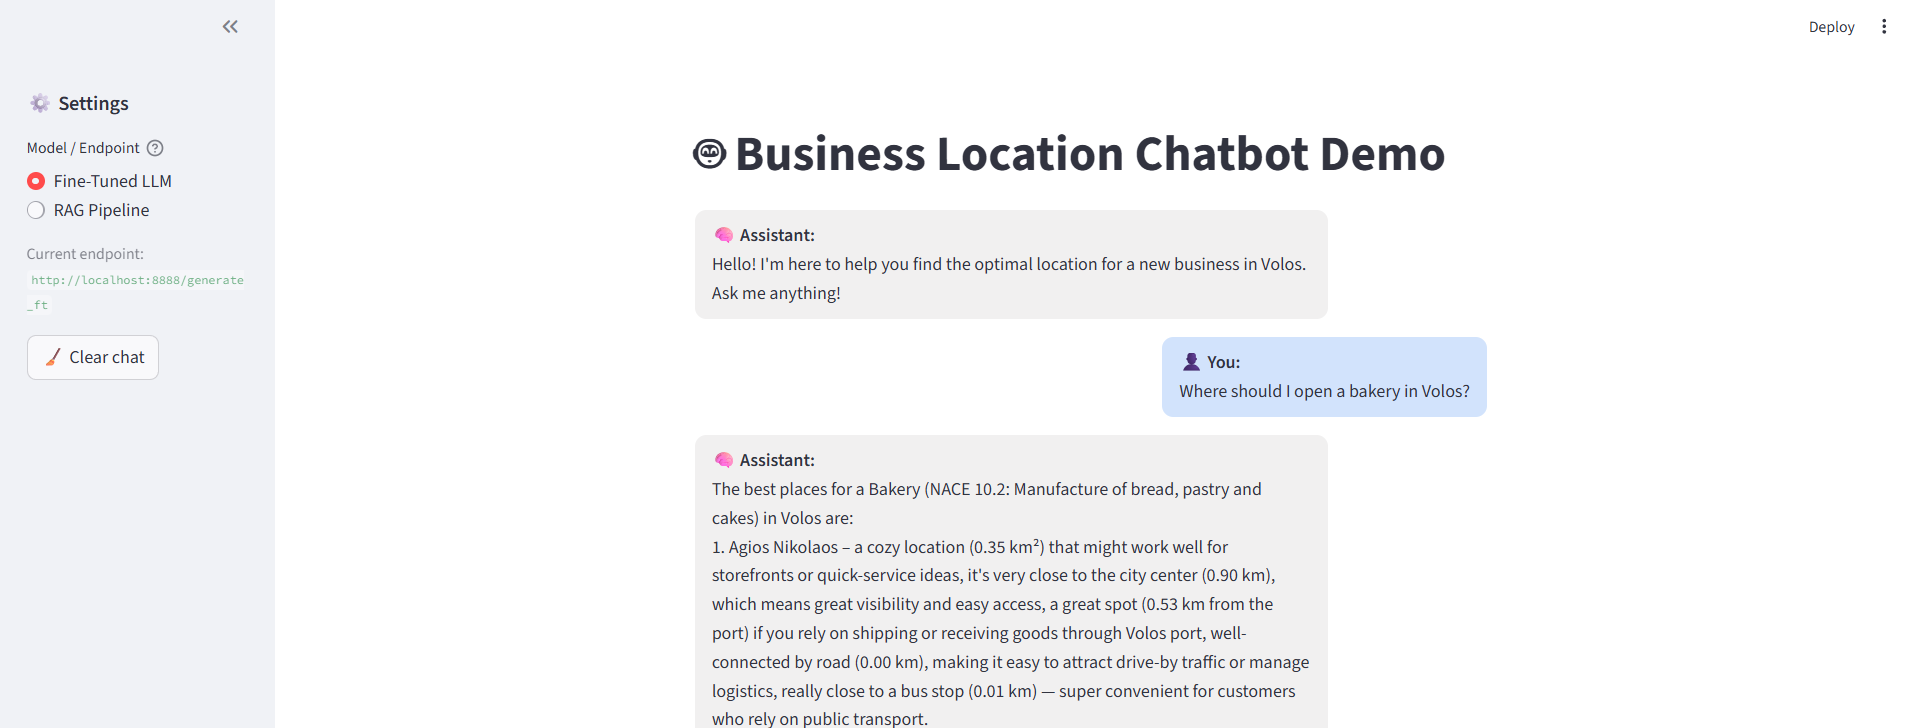
\includegraphics[width=0.8\textwidth]{figures/inf_chatbot_ft_1.png}\\[0.5em]
    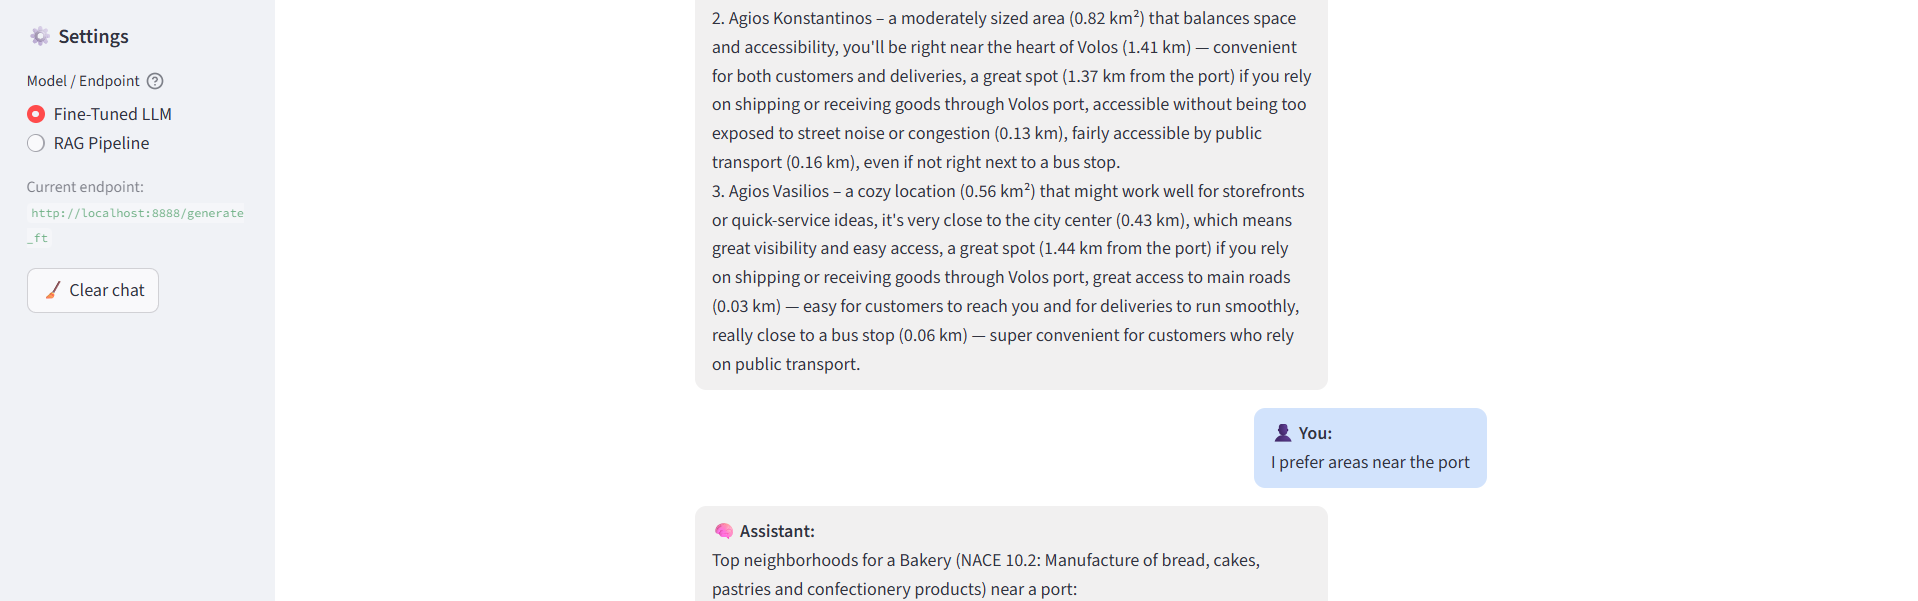
\includegraphics[width=0.8\textwidth]{figures/inf_chatbot_ft_2.png}
    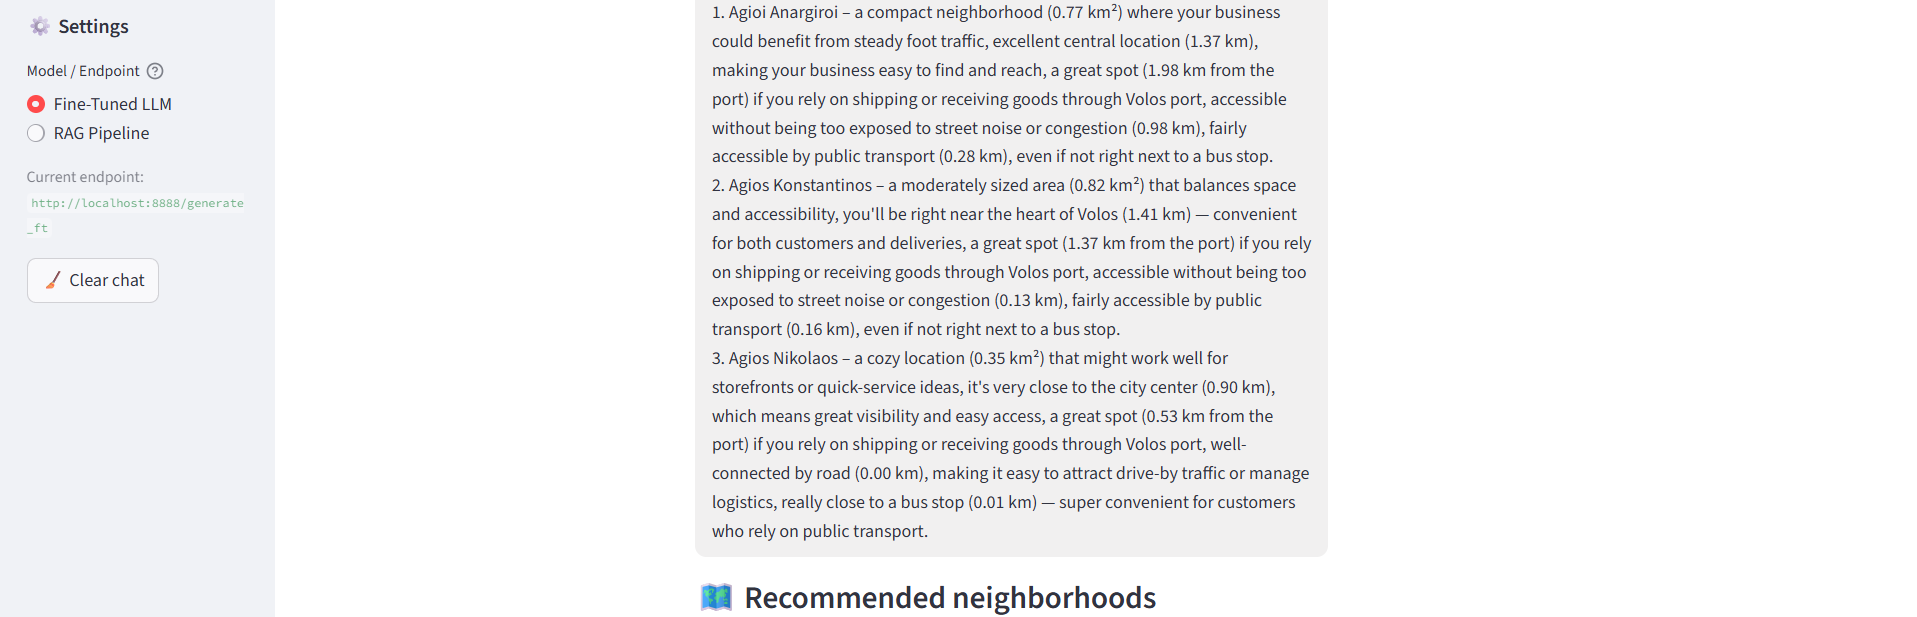
\includegraphics[width=0.8\textwidth]{figures/inf_chatbot_ft_3.png}
    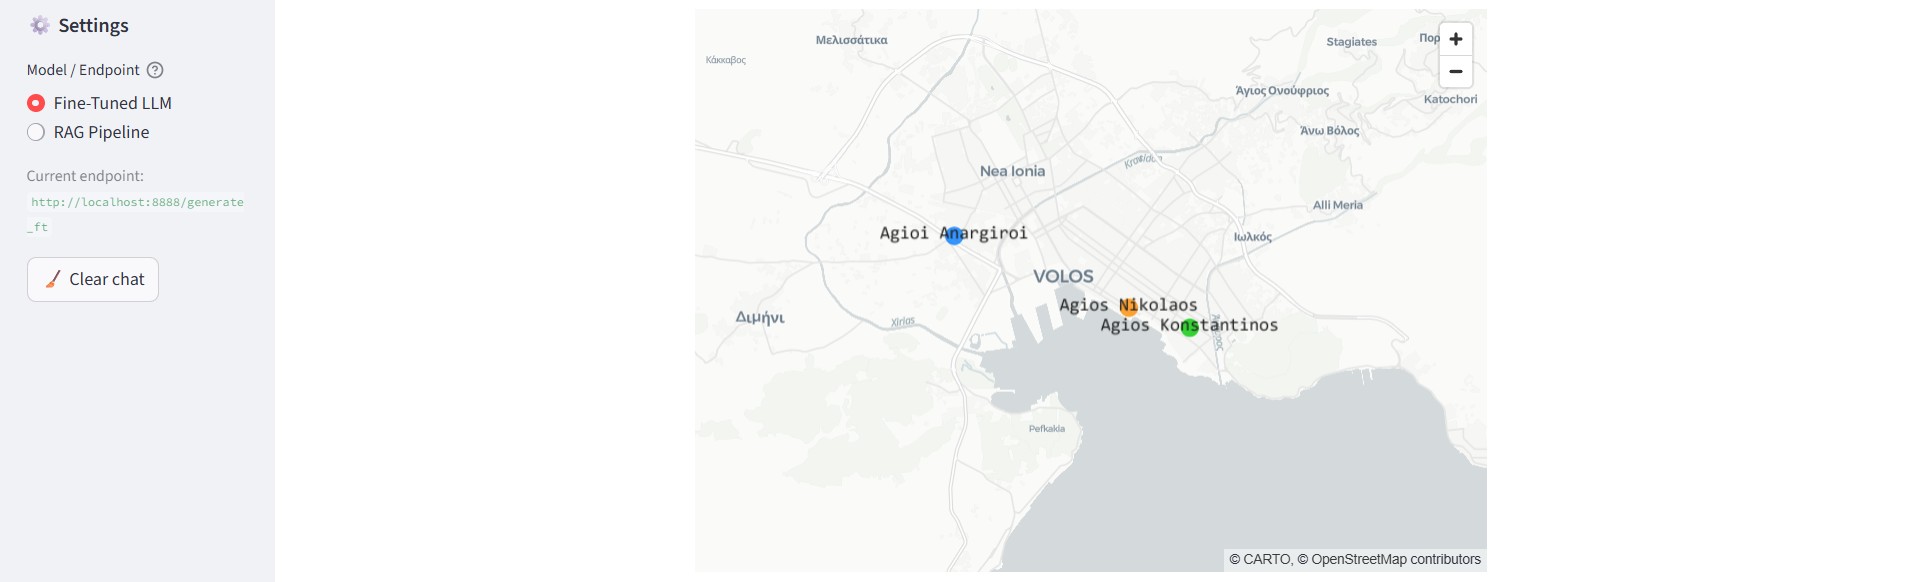
\includegraphics[width=0.8\textwidth]{figures/inf_chatbot_ft_4.png}
    
\includegraphics[width=0.8\textwidth]{figures/inf_chatbot_ft_5.png}
    \caption{Chatbot Inference - Fine-Tuned LLM Approach}
    \label{fig:chatbot_inf_ft}
\end{figure}



%==================================================
\subsubsection{RAG Pipeline Approach}

Figure \ref{fig:chatbot_inf_rag} shows an instance of  the conversation that occurs by the RAG pipeline. In contrast with the fine-tuned LLM, this output follows a slightly different reasoning format because the generator is not trained on following the structure of the training data. This time the chatbot actually changes its prediction in the correct direction, as the port distance constraint produces Palaia as the first recommendation, which is closer to the port than the old recommendation. 


\begin{figure}[h!]
    \centering
    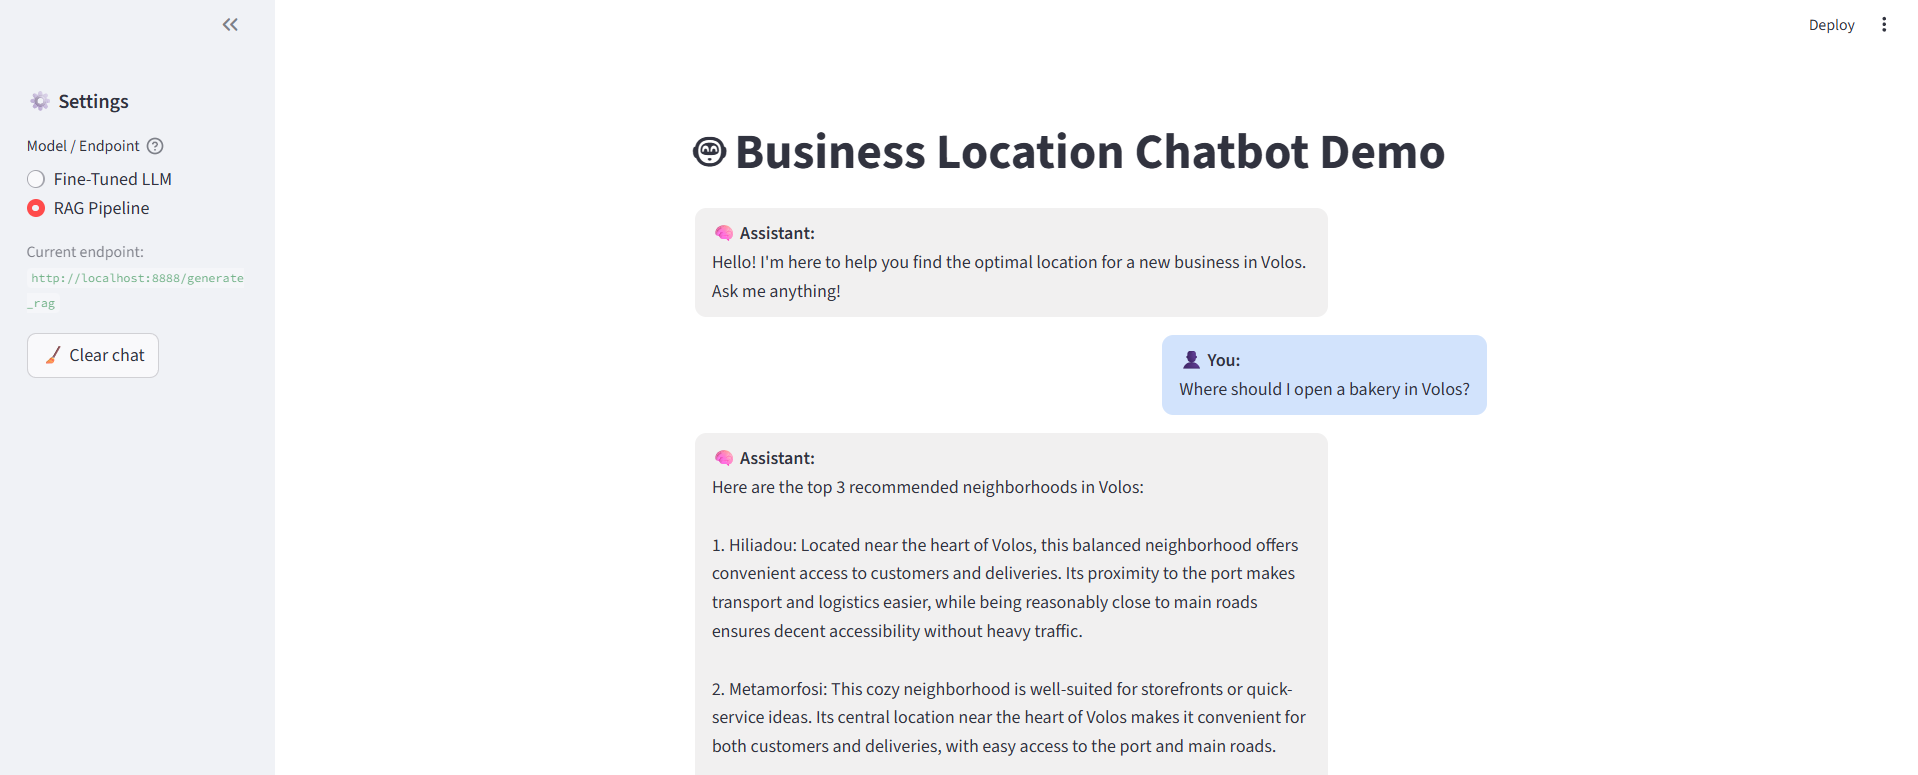
\includegraphics[width=0.8\textwidth]{figures/inf_chatbot_rag_1.png}\\[0.5em]
    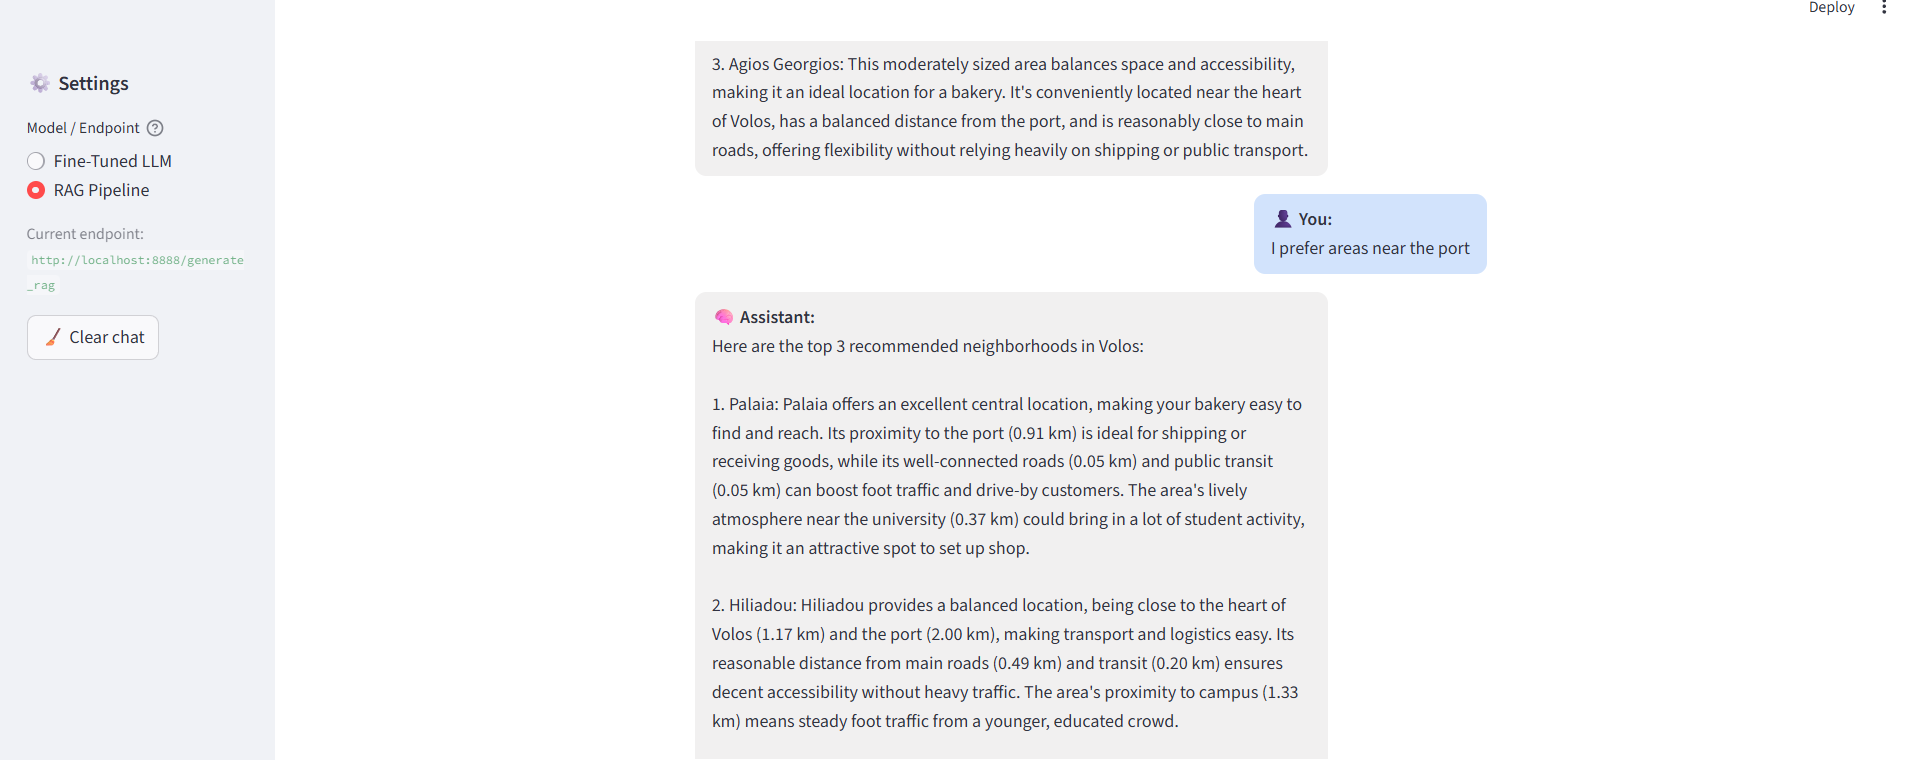
\includegraphics[width=0.8\textwidth]{figures/inf_chatbot_rag_2.png}
    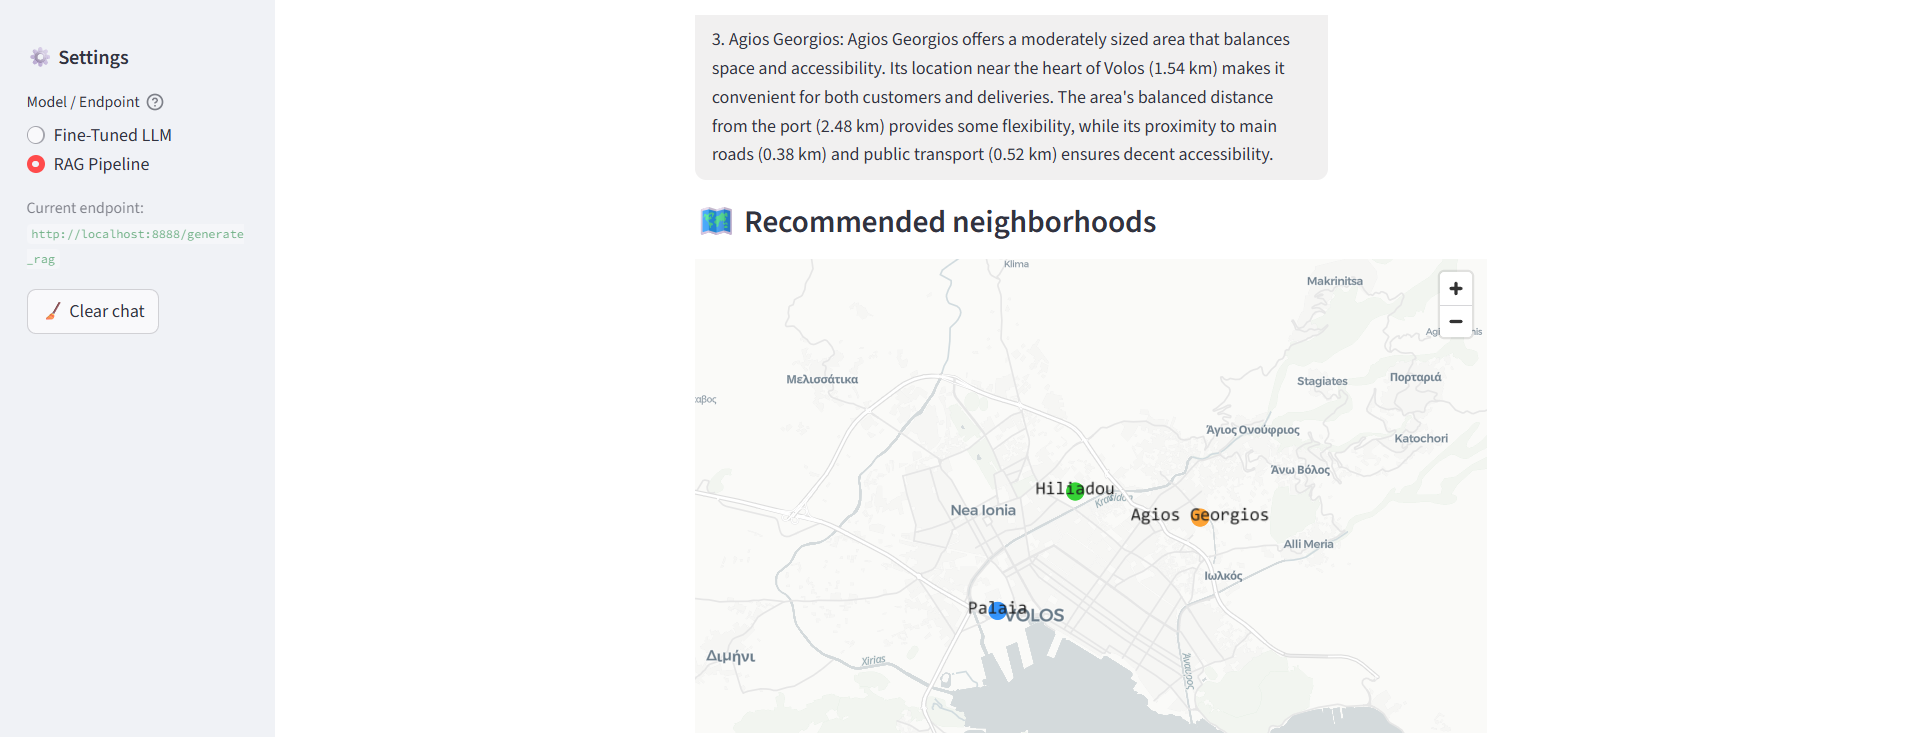
\includegraphics[width=0.8\textwidth]{figures/inf_chatbot_rag_3.png}
    
\includegraphics[width=0.8\textwidth]{figures/inf_chatbot_rag_4.png}
    \caption{Chatbot Inference - RAG Pipeline Approach}
    \label{fig:chatbot_inf_rag}
\end{figure}
    \chapter{Experiments and Results}
\label{chap5}


In this chapter, we describe the evaluation and comparison of the fine-tuned LLM and Retrieval-Augmented Generation systems. We begin by specifying the environment configurations, then proceed to mention the evaluation metrics, and finally calculate those metrics to evaluate and compare both approaches. 


%==================================================
%==================================================
%==================================================
\section{Experimental Setup}


Here, we present details of the setup of the evaluation process. First and foremost, we aim to evaluate two approaches: the fine-tuned LLM, and the RAG system. We tested both frameworks on simple input-output pairs that aim to measure their quality as regular LLMs, not as chatbots. They were tested on the same dataset, specifically the 'inference dataset', constructed in section \ref{sec:inference_dataset}, which contains 159 entries Each entry consists of one prompt, which will be used as the input to each system, and its corresponding proxy truth output, which will be compared to the system prediction. 

During evaluation, the fine-tuned LLM inference was performed on a remote server provided by the University of Thessal equipped with an NVIDIA A100 GPU with 40 GB of VRAM and 128 GB of RAM. This was performed on an Ubuntu environment using Python 3.10.12 and the Transformers library from Hugging Face. The RAG experiments were carried out locally (HP OMEN Laptop 15-en0xxx) on Windows 11 operating system, equipped with an AMD Ryzen 7 4800H CPU 16 GB RAM, without the use of a dedicated GPU. The environment contained Python 3.9.18, with the Ollama library employed as well.


%==================================================
%==================================================
%==================================================
\section{Evaluation Metrics}

To evaluate the performance of both approaches, several complementary accuracy metrics were utilized. Certain metrics examine semantic similarity, while others measure recommendation quality. In addition, we provide an efficiency metric that measures system inference speed.



%==================================================
%==================================================
\subsection{Recommendation Metrics}

To evaluate the quality of system recommendations, we apply metrics that measure how close they are to their corresponding proxy ground truths. These metrics are widely used in recommendation systems and information retrieval evaluation.


\begin{itemize}
    \item \textbf{Match@3:} captures whether at least one of the three provided recommendations belongs in the proxy truth set, providing a measure of minimal success

    \item \textbf{Precision@3:} evaluates the proportion of the three predicted locations that are correct, emphasizing on the on the quality of the recommendations

    \item \textbf{Recall@3:} measures the proportion of the proxy ground truths that the top three recommendations manage to capture, emphasizing on the system’s ability to cover the expected solutions
\end{itemize}



%==================================================
%==================================================
\subsection{Semantic Metrics}

In addition to evaluating the actual system recommendations, it is also important to measure the semantic similarity between the predicted completions and the proxy ground truths. This could evaluate the system justification, ensuring that different wording that results in similar context does not get penalized. To acquire these metrics, we used BERT-score, which generates embeddings from the pre-trained transformer model 'RoBERTa-large'. For every token of the predicted output, the most similar token of its corresponding reference is found, and the following three metrics are calculated:


\begin{itemize}
    \item \textbf{Precision}: measures the proportion of the predicted output's tokens that have a semantically close match in its corresponding proxy truth

    \item \textbf{Recall}: measures the proportion of the proxy truth's tokens that are covered in the generated completion  

    \item \textbf{F1}: the harmonic mean of precision and recall metrics, providing a balanced similarity score
\end{itemize}


%==================================================
%==================================================
\subsection{Efficiency Metric}
\label{sec:metrics}

In addition to evaluating the quality of the recommendations, we also considered measuring the efficiency of each system. This metric demonstrates the computational trade-offs between the two approaches.

\begin{itemize}
    \item \textbf{Inference Time per Query}: the average inference time of the system, measures practical system responsiveness
\end{itemize}


%==================================================
%==================================================
%==================================================
\section{Results of Fine-Tuned LLM}


For the fine-tuned LLM approach, I attempted multiple trainings that use a different number of epochs. Specifically, we used 3, 5, and 8 epochs. This was done to ensure that the training process was neither interrupted too soon nor led to model overfitting. Figure \ref{fig:comparison_fine_tuned} demonstrates estimations of the metrics explained in section \ref{sec:metrics}. The complete values of the evaluation metrics are displayed in table \ref{tab:results_ft}.

\begin{figure}[h]
    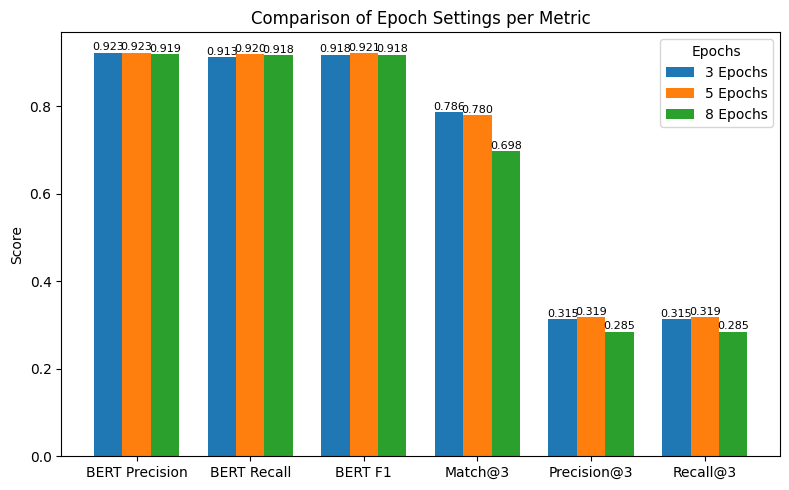
\includegraphics[scale=0.45]{figures/comparison_fine_tuned.png}
    \centering
    \caption{Fine-Tuned Models Comparison}
    \label{fig:comparison_fine_tuned}
\end{figure}


As we see, after 8 epochs every metric decreases. This indicates that the model starts to overfit and should not be further trained on our data. The semantic similarity metrics are generally higher than the recommendation metrics for every attempt. This implies that the justifications are satisfying and semantically close to the proxy truths across all the models. If we observe the BERT-F1 value, which acts as a harmonic mean of the other two metrics, it slightly peaks at 5 epochs. Regarding the recommendation metrics, we see that Match@k has higher values than Precision@3/Recall@3, which is expected since it is a less strict metric. Although the highest Match@k value occurs at 3 epochs, if we also look at Precision@3/Recall@3, the complete recommendation accuracy peaks at 5 epochs. This indicates that the model more often retrieves at least one correct community, but is less precise overall.

The overall trend shows that the metrics tend to increase from 3 to 5 epochs, but the performance decreases significantly at 8 epochs. This indicates that the model can be further trained on the fine-tuning data after 3 epochs, but overfits at 8 epochs. Overall, 5 epochs represent the optimal fine-tuning configuration among the tested attempts. This is the fine-tuned LLM we select to be integrated to the chatbot system. 

%==================================================
%==================================================
%==================================================
\section{Results of RAG System}

The RAG pipeline is parametrized by certain components, as the embedder and generative LLM models used. In our case, we chose to modify the neighborhood descriptions to demonstrate the dynamic nature of the system. As described in section \ref{sec:neigh_desc}, we can specifically select the number of feature justifications included in the neighborhood description. We implemented three attempts, with 10, 15, and 20 justifications, respectively. Since the descriptions represent the system memory, modifying them also shows the ability of the framework to change its memory without the need for additional training. Figure \ref{fig:comparison_rag} compares the metrics for the different attempts. The complete values of the evaluation metrics are displayed in table \ref{tab:results_rag}.

\begin{figure}[h]
    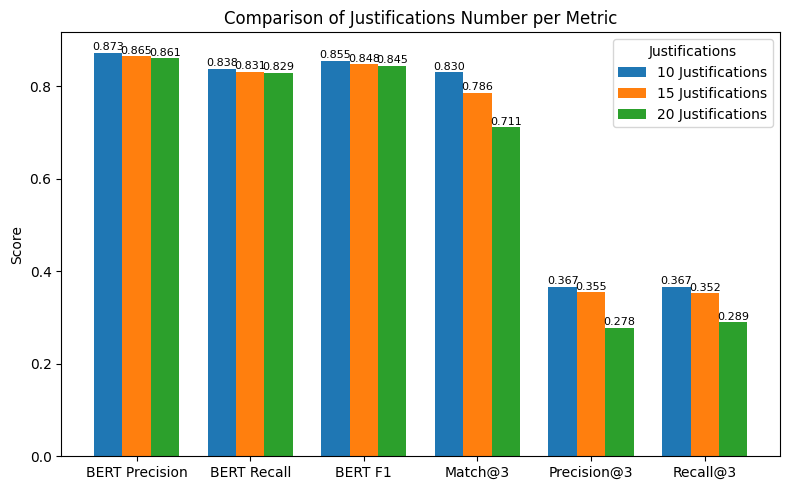
\includegraphics[scale=0.45]{figures/comparison_rag.png}
    \centering
    \caption{RAG Systems Comparison}
    \label{fig:comparison_rag}
\end{figure}

We observe that the quality drops as the justifications, and therefore the length of neighborhood descriptions, increases. In our RAG pipeline, the accuracy of the system is determined by the accuracy of NACE class prediction, which in turn depends on the embedder model. This implies that, in general, the embedder performance worsens as the size of the descriptions increases. Mutiple factors could contribute to this tendency. Firstly, the encoder has a token limit, beyond which everything gets truncated.  If important information is added to the end of the description, it can get cut off and never get embedded, unless we use chunking, which we do not in our case. In addition, the description embedding is created by averaging the embeddings of its tokens. Adding irrelevant tokens results in weaker description embeddings. This suggests that the extra details are either not that relevant to the descriptions, or introduce semantic noise. In our chatbot, we will keep the descriptions that include 10 justifications.



%==================================================
%==================================================
%==================================================
\section{Comparison of Approaches}


To compare the two systems, we selected the best attempt to represent each approach. These are: the LLM fine-tuned on 5 epochs, and the RAG pipeline that uses neighborhood descriptions that include 10 justifications. In addition to the semantic and recommendation metrics demonstrated in the previous paragraph, we include the efficiency metric to highlight the computational trade-offs of the two approaches. Figure \ref{fig:comparison_ft_rag} demonstrates the semantic and recommendation metrics between the two systems. These values can also be found in table \ref{tab:results_ft_rag}. In addition, the efficiency metric is shown in Figure \ref{fig:comparison_ft_rag_time}, while table \ref{tab:results_ft_rag_time} contains the analytical time-related values.

\begin{figure}[h]
    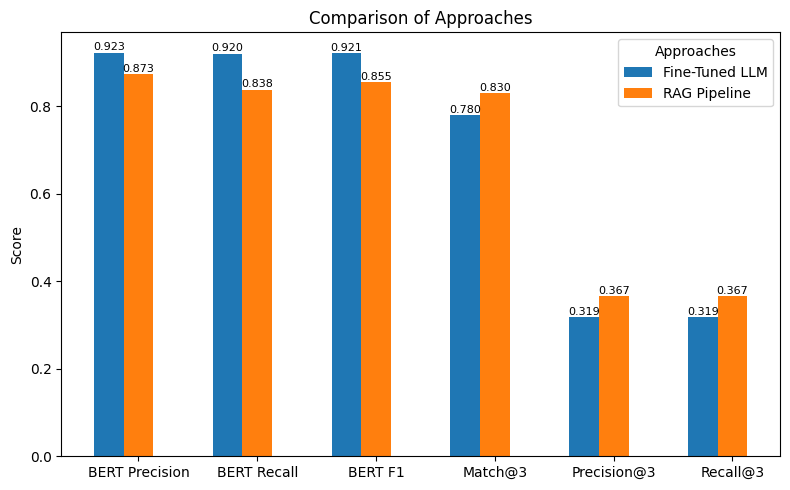
\includegraphics[scale=0.45]{figures/comparison_ft_rag.png}
    \centering
    \caption{Comparison of Approaches - Semantic \& Recommendation Metrics}
    \label{fig:comparison_ft_rag}
\end{figure}

\begin{figure}[h]
    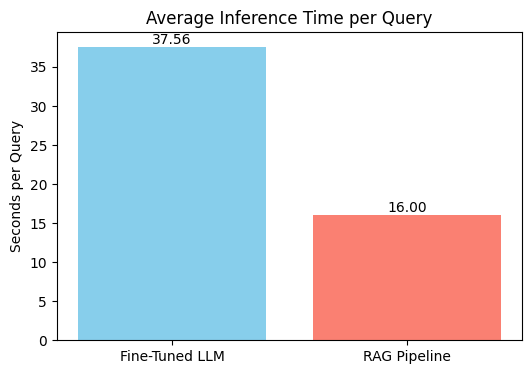
\includegraphics[scale=0.45]{figures/comparison_ft_rag_time.png}
    \centering
    \caption{Comparison of Approaches - Efficiency Metric}
    \label{fig:comparison_ft_rag_time}
\end{figure}


Overall, BERT scores are higher for the fine-tuned system. In contrast, the recommendation metrics tend to favor the RAG pipeline. The efficiency metric also demonstrates the quicker inference of the fine-tuned model. Both approaches present significant strengths and limitations, which will be further analyzed below.


%==================================================
%==================================================
%==================================================
\section{Chatbot Performance}

In the previous sections. we evaluated and compared the performance of our two LLM-based approaches. Although these results are insightful, the performance of the system is slightly affected when they are integrated into a chatbot application. In particular, we see that the RAG approach is actually faster during conversation.

This happens because the inference of the evaluation dataset used a batch size of 8, which utilized the available GPU much more efficiently than the current one-to-one conversation setting. This can also be attributed to the difference in input size between the two approaches.  As explained in \ref{sec:backend_ft}, the fine-tuned LLM input is the combination of all previous user messages, which increases in length as the conversation progresses. In contrast, the RAG input is structured upon a fixed template, regardless of the past messages \ref{sec:backend_rag}. Because the response time of an LLM is proportional to the input size, the fine-tuned LLM carries a greater computational burden.




%==================================================
%==================================================
%==================================================
\section{Conclusions}

In the previous paragraph, we presented the results of the comparison of the two methods. Here, we interpret these metrics to extract general insights on the strengths and weaknesses of each system. We also mention limitations met throughout this thesis, and possible future directions that could enhance the project even more.

%==================================================
%==================================================
\subsection{Summary of Key Findings}


The result of the comparison showed that the semantic similarity is better captured by the fine-tuned LLM. This approach also provides faster inference, which is expected since it uses only one model and utilizes the GPU better by using a batch size of 8. In contrast, the RAG framework demonstrated greater adaptability, along with high accuracy in capturing recommendations. This happens because the accuracy of the RAG system depends entirely on the embedder performance, which provides the correct recommendations if it captures the NACE class successfully. The semantic metrics probably have worse values because RAG does not use the pure proxy justifications, but the reasoning is influenced by the generative LLM. Both approaches have distinct advantages depending on the deployment scenario. The dilemma between them demonstrates a clear trade-off between static efficiency and dynamic adaptability.

The chatbot application demonstrates a different outcome regarding the speed of the fine-tuned LLM approach. Since the structure of the conversation contains a single query, we cannot use batching and therefore utilize the GPU fully. On the other hand, the flexibility of the RAG pipeline allows the designer to select different generator models. In our case, we use Ollama, which optimizes the Llama3 LLM. Additionally, a chatbot application uses memory to provide context to follow-up replies. While the RAG system is based on a pre-defined template, the fine-tuned LLM integrates past user messages, resulting in a larger input, which burdens its performance.

%==================================================
%==================================================
\subsection{Strengths and Limitations of each Approach}


The core idea of the Fine-tuned LLM system is to train an LLM to directly generate business location recommendations with justifications. Since the framework relies on a single large model, predicting new outputs requires only one inference, making the process fast. In addition, considering that the model is trained on domain-specific data, it learns patterns that allow it to generalize to unseen prompts. However, given that the knowledge of the model depends almost entirely on the fine-tuning data, keeping the model up to date (e.g. learning new NACE classes or updated proxy truths) requires re-training, which is a computationally expensive process. Furthermore, since the generated completions depend on the weights of the model, it is prone to hallucinations, by providing incorrect data in the justifications. Finally, given that the model learns static suggestions for every NACE class, it may lack in utilizing user preferences to provide personalised recommendations.


The RAG pipeline, on the other hand, uses embeddings to first extract the NACE class, and then retrieve relevant neighborhoods and re-rank them, based on their similarity to the user query. This method makes better use of the user specifications, and reduces hallucinations, as the generative LLM is fed the justifications in real time. Moreover, the flexible structure of this system allows us to simply update the neighborhood descriptions without the need to re-train. Nevertheless, this method presents a number of limitations. Its main disadvantage is its slower inference, due to the overhead of the real-time embedding of the user query and the retrieval process. It also requires additional infrastructure to store the descriptions and the embeddings, and its dependence on the embedder quality can harm the total system performance.

The integration of the approaches into a chatbot application introduced new parameters about their appropriateness. As the conversation structure follows a one-to-one message, a single-threaded application does not fully utilize the GPU resources. However, as the fine-tuned LLM inference demonstrated, concurrent queries could enable the full potential of the GPU parallel computing. This could correspond to a scenario of a real-life server that receives multiple queries simultaneously and utilizes a batch to process them in parallel.

Both systems provide significant and promising results, but we cannot definitively argue that one is superior to the other. Rather, each method is better suited for different conditions and circumstances. For example, startups that still determine the best recommendation per NACE class and require dynamic updates might prefer the RAG pipeline. If the most important concern is speed, or we desire to withstand concurrent queries or batched workloads, the fine-tuned LLM might be the best solution. Table \ref{tab:comparison_ft_rag} describes the trade-offs between the approaches in detail.



    \chapter{Conclusions and Discussion}
\label{chap6}



In this chapter, we provide a comprehensive review of the results of this thesis and draw our final conclusions about the bigger picture. We also mention several future directions that can potentially enhance the application even more.


%==================================================
%==================================================
%==================================================
\section{Summary of Key Findings}

This thesis began by constructing the three main datasets of the project. This process involved merging heterogeneous data structures from multiple sources, extracting additional information from software applications, and combining and analyzing the final dataset, which joins business records with geographical, economic, and demographic characteristics. This dataset provided the basis for creating proxy ground truths to evaluate business location suitability.

Two state-of-the-art frameworks were introduced and developed. Firstly, a fine-tuned LLM was trained on a constructed domain-specific dataset. Next, a RAG pipeline that required the creation of descriptions of neighborhoods for the retrieval was implemented. The fine-tuning dataset and neighborhood descriptions provided justifications about the recommendations, created through the use of explainable AI methods. Both approaches were evaluated on the same data with the same metrics.

To transform the LLM-based systems into user-friendly frameworks that support personalization, a chatbot application that offers the option for both predictive systems was implemented. The two approaches acted as the application backend, which communicated with a user interface that stores and transfers the entire conversation history.

Overall, the two approaches demonstrated a trade-off between efficiency and accuracy. While the fine-tuned LLM can easily generalize to unseen data efficiently and fully utilize the GPU resources during concurrent requests, the RAG system provides better adaptability, lowers hallucination risk, and enables dynamic memory updating without the need for re-training. Each approach is therefore suited to different deployment contexts. The user can select the backend system depending on the nature of the application.

%==================================================
%==================================================
\section{Limitations}

In the course of this project, several challenges were faced. First and foremost, the recommendations per NACE class are approximations that were estimated by ensembling three weaker approaches. If actual ground truths were available, the results of the recommendation system would be much more reliable and valuable. In addition, although we believe that the dataset used represents the business tendencies of the city, it is relatively small (less than 4.000 entries). A larger dataset could potentially lead to different, more realistic conclusions. Our hardware constraints also limit the potential system accuracy. Moreover, larger and better models, either generative for fine-tuning, or embedding encoder for retrieval, could improve the performance of the systems.


%==================================================
%==================================================
\section{Future directions}

To improve the recommendation system, there are multiple potential enhancements that could be explored in the future. Acquiring ground truths would be a fundamental improvement in order to escape from estimating the optimal locations and provide realistic recommendations. More base models could be explored for the fine-tuned LLM approach, potentially with more parameters. The model quality is also largely influenced by the fine-tuning dataset, which can be enhanced if more business data is gathered. Using more synthetic categories per NACE class to create a training dataset with more entries may also lead to a more domain-specific model. The fine-tuning dataset could also be improved through the use of prompt engineering, as is the case for the creation of the neighborhood descriptions used in RAG. The RAG pipeline could be improved if we explored different embedder models. In addition, since current embeddings are stored locally in files, techniques like chunking and utilizing vector databases could possibly allow the system to use larger neighborhood descriptions successfully. Finally, regarding the chatbot application, a database could be set up to store and retrieve past conversation sessions. In addition, the current structure uses one server for both approaches, which could be modified into multiple servers to make the application more modular and scalable.


%==================================================
%==================================================
\section{Conclusions}


This thesis focused on integrating spatial information such as economic, demographic, and geographical data with generative AI technologies like LLMs for optimal business recommendation. By comparing two cutting-edge algorithms -LLM fine-tuning and Retrieval-Augmented Generation- we identified complementary strengths and weaknesses that mirror potential use cases in real-world examples. We believe this thesis can serve as a foundation for further improving business recommendation by combining spatial information with state-of-the-art methodologies.

%
%%%%%%%%%%%%%%%%%%%%%%%%%%%%%%%%%%%%%%%%%%%%%%%%%%%%


%\backmatter % μην ενεργοποιείτε την εντολή
% Βιβλιογραφία - Αναφορές
	\bibliography{references}


%%%%%%%%%%%%%%%%%%%%%%%%%%%%%%%%%%%%%%%%%%%%%%%%%%%%%
%% APPENDICES (optional) / ΠΑΡΑΡΤΗΜΑΤΑ (ΠΡΟΑΙΡΕΤΙΚΑ)
%%

% Εάν υπάρχουν περισσότερα από ένα Παραρτήματα
% είναι ενεργή η ακόλουθη εντολή
% και ανενεργή για μεμονωμένο Παράρτημα
    \include{appendices}

% Μην τροποποιήσετε τις ακόλουθες εντολές
\ifgrthesisoption
    \renewcommand{\chaptername}{Παράρτημα}
\else
    \renewcommand{\chaptername}{Appendix}
\fi

% Πριν το κάθε Παράρτημα (για περισσότερα από ένα), 
% ρυθμίζεται η κατάλληλη αλφαβητική αρίθμηση
    
    \renewcommand{\thechapter}{A}
    % Παράρτημα A

\chapter{Datasets Structure \& Analysis}


%========================================
%========================================
%========================================
\section{Business Entries Dataset}

This appendix contains information about the business dataset after unifying the entries from multiple sources, filling the missing values, and adding the NACE code:

%========================================
%========================================
\subsection{Dataset Structure}

This section provides the structure of the pure business dataset (before joining).

\begin{longtable}{p{5cm} p{10cm}}
    \caption{Business Dataset Columns (highlighted features are used for joining)} \label{tab:business_columns} \\
    \hline
    \textbf{Column Name} & \textbf{Description} \\
    \hline
    \endfirsthead
    
    \multicolumn{2}{c}{{\bfseries Table \thetable\ (continued)}} \\
    \hline
    \textbf{Column Name} & \textbf{Description} \\
    \hline
    \endhead
    
    \hline \multicolumn{2}{r}{{Continued on next page}} \\
    \endfoot
    
    \hline
    \endlastfoot
    
    Name & Business name as listed in the source dataset \\
    Category & General business category (e.g., restaurant, retail, service) \\
    Latitude & Geographic latitude coordinate of the business location \\
    Longitude & Geographic longitude coordinate of the business location \\
    Address & Full street address of the business \\
    Country & Country where the business is located \\
    City & City where the business is located \\
    Postal Code & Postal code of the business location \\
    Rating & Average rating score given by customers, if available \\
    Reviews & Number of customer reviews, if available \\
    Source & Origin of the business entry \\
    Description & Short textual description of the business \\
    NACE Code & Official NACE classification code for the business activity \\
    NACE Description (EN) & English description of the NACE code activity \\
    \rowcolor{yellow!20}
    Municipal Community & The municipal community of the business location\\
    \rowcolor{yellow!20}
    Neighborhood & The neighborhood of the business location\\
    
\end{longtable}

%========================================
%========================================
\subsection{Dataset Analysis}


\subsubsection{Feature Values Distributions}

Here we see the most frequent values of the business dataset features that were not explicitly mentioned in the paragraph \ref{EDA_business}.

\begin{figure}[h]
    \centering
    \begin{minipage}[b]{0.45\textwidth}
        \centering
        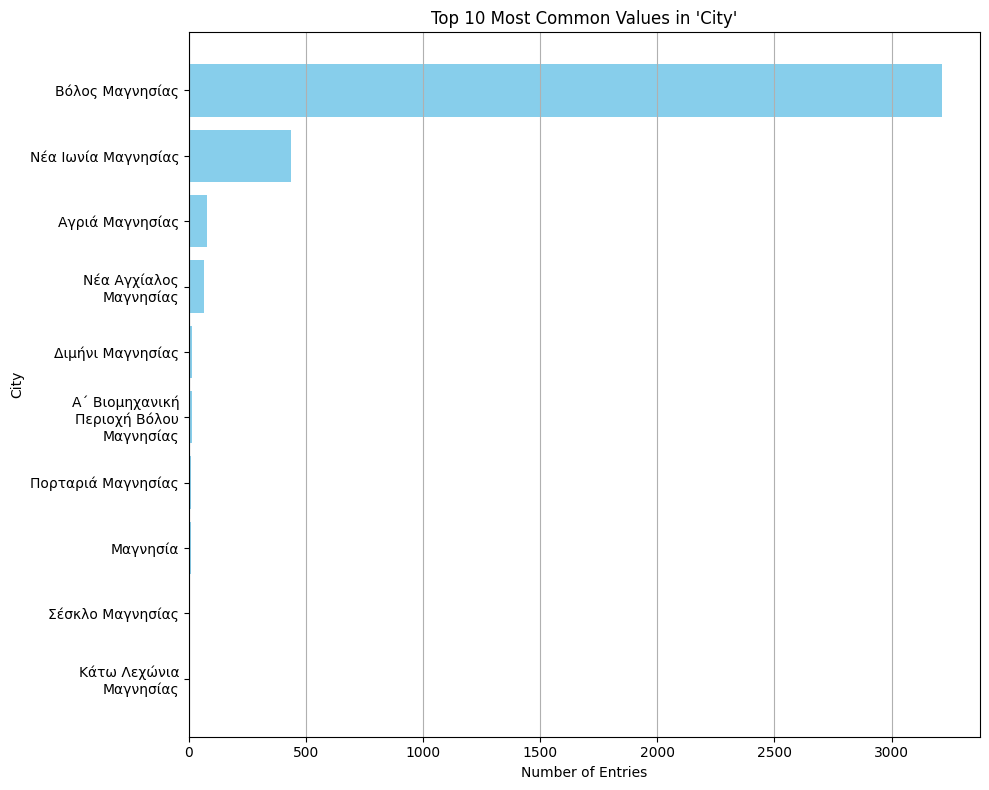
\includegraphics[height=5cm]{figures/distribution_city.png}
        \caption{'City' Bar Chart}
        \label{fig:city_distr}
    \end{minipage}
    \hfill
    \begin{minipage}[b]{0.45\textwidth}
        \centering
        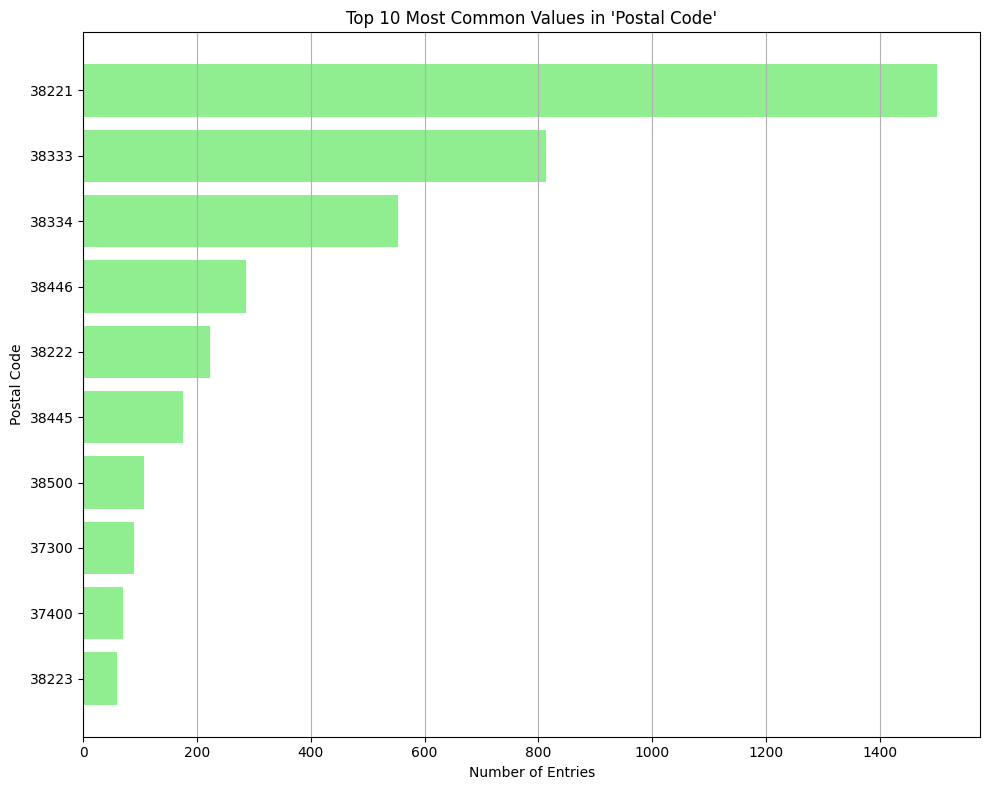
\includegraphics[height=5cm]{figures/distribution_postal_code.png}
        \caption{'Postal Code' Bar Chart}
        \label{fig:postal_distr}
    \end{minipage}
\end{figure}

\begin{figure}[h]
    \centering
    \begin{minipage}[b]{0.45\textwidth}
        \centering
        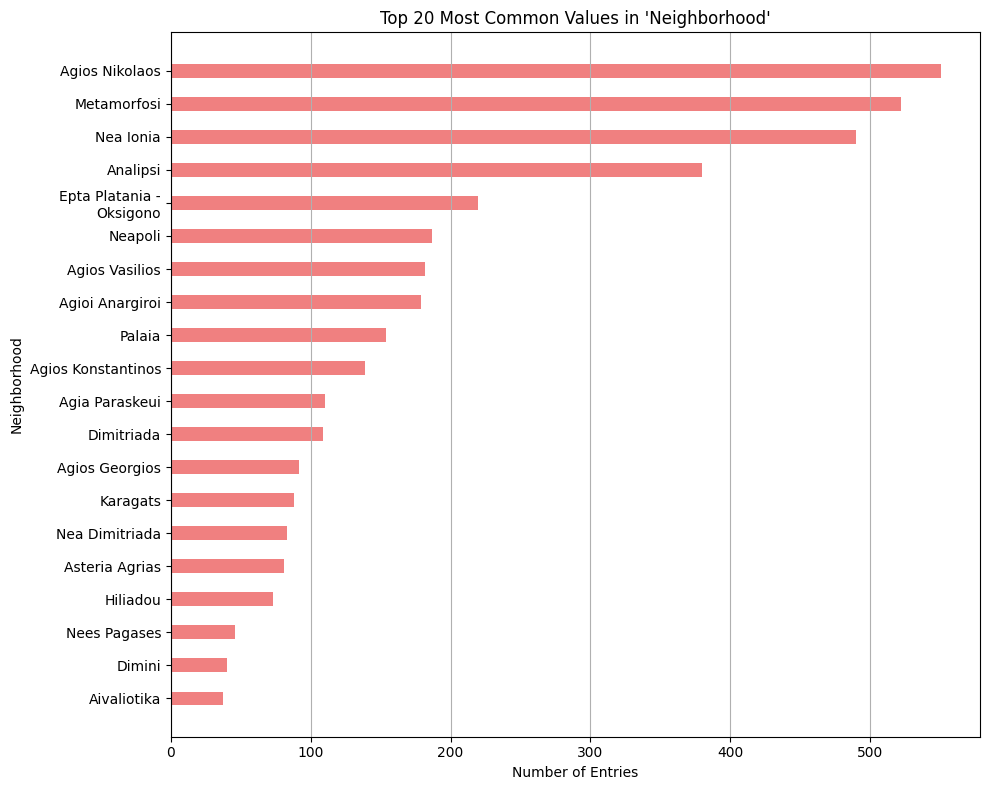
\includegraphics[height=5cm]{figures/distribution_neighborhoods.png}
        \caption{'Neighborhood' Bar Chart}
        \label{fig:neighborhood_distr}
    \end{minipage}
    \hfill
    \begin{minipage}[b]{0.45\textwidth}
        \centering
        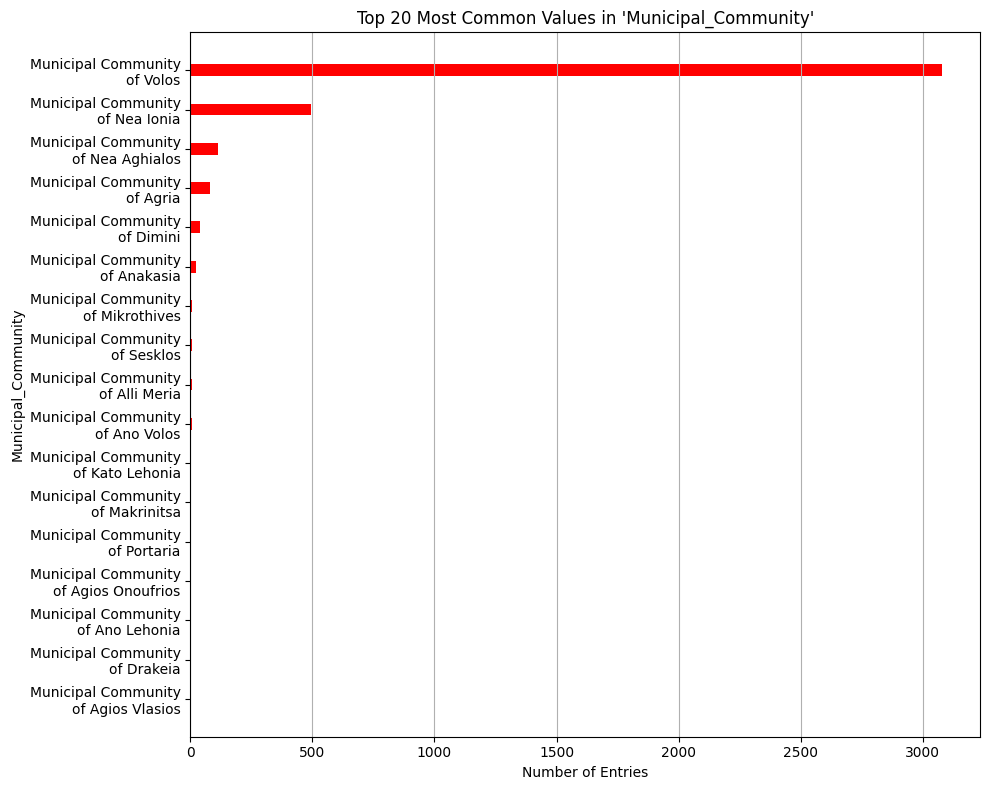
\includegraphics[height=5cm]{figures/distribution_mc.png}
        \caption{'MC' Bar Chart}
        \label{fig:mc_distr}
    \end{minipage}
\end{figure}

\begin{figure}[h]
    \centering
    \begin{minipage}[b]{0.45\textwidth}
        \centering
        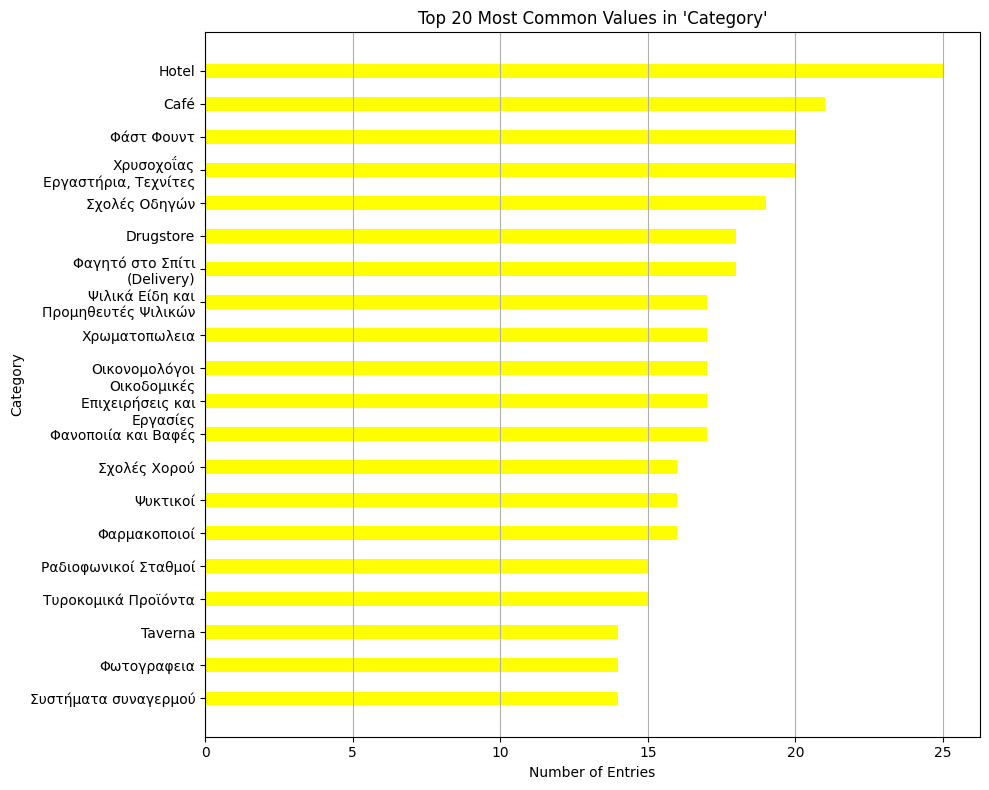
\includegraphics[height=5cm]{figures/distribution_category.png}
        \caption{'Category' Bar Chart}
        \label{fig:category_distr}
    \end{minipage}
    \hfill
    \begin{minipage}[b]{0.45\textwidth}
        \centering
        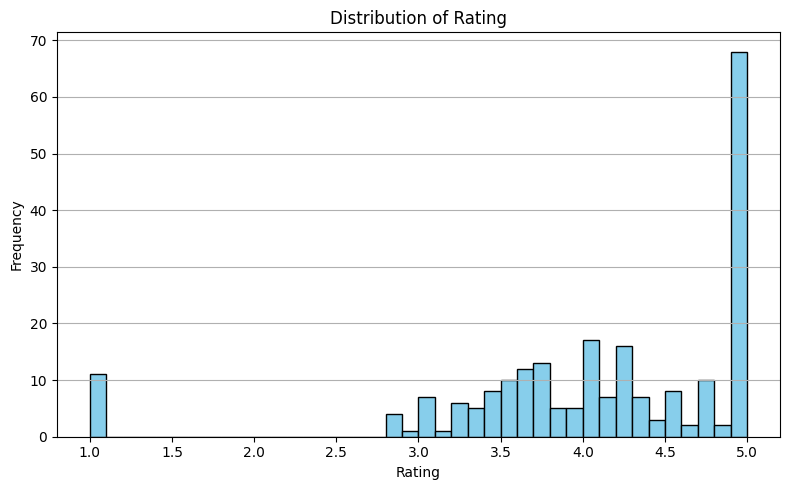
\includegraphics[height=5cm]{figures/distribution_rating.png}
        \caption{'Rating' Histogram}
        \label{fig:distr_rating}
    \end{minipage}
\end{figure}



%========================================
%========================================
%========================================
\newpage
\section{ELSTAT Datasets}

This appendix contains information about the data extracted from the ELSTAT platform: their raw structure, visualizations about their analysis, and more.

%========================================
%========================================
\subsection{Datasets Structure}

Here we present the complete structure of the raw demographic and economic data extracted from the ELSTAT platform.


%========================================
\subsubsection{Raw Demographic Data}

\begin{longtable}{p{5cm} p{10cm}}
    \caption{Demographic Dataset Columns} \label{tab:demographic_columns} \\
    \hline
    \textbf{Column Name} & \textbf{Description} \\
    \hline
    \endfirsthead
    
    \multicolumn{2}{c}{{\bfseries Table \thetable\ (continued)}} \\
    \hline
    \textbf{Column Name} & \textbf{Description} \\
    \hline
    \endhead
    
    \hline \multicolumn{2}{r}{{Continued on next page}} \\
    \endfoot
    
    \hline
    \endlastfoot
    
    ΠΕΡΙΦΕΡΕΙΑΚΗ ΕΝΟΤΗΤΑ & Administrative regional unit where the municipal community belongs \\
    ΔΗΜΟΣ & Municipality name \\
    ΔΗΜΟΤΙΚΗ ΕΝΟΤΗΤΑ & Administrative municipal unit \\
    ΔΗΜΟΤΙΚΗ ΚΟΙΝΟΤΗΤΑ & Administrative municipal community name (Greek) \\
    Population & Total population count \\
    0-4 & Population aged 0 to 4 years \\
    5-9 & Population aged 5 to 9 years \\
    10-14 & Population aged 10 to 14 years \\
    15-19 & Population aged 15 to 19 years \\
    20-24 & Population aged 20 to 24 years \\
    25-29 & Population aged 25 to 29 years \\
    30-34 & Population aged 30 to 34 years \\
    35-39 & Population aged 35 to 39 years \\
    40-44 & Population aged 40 to 44 years \\
    45-49 & Population aged 45 to 49 years \\
    50-54 & Population aged 50 to 54 years \\
    55-59 & Population aged 55 to 59 years \\
    60-64 & Population aged 60 to 64 years \\
    65-69 & Population aged 65 to 69 years \\
    70-74 & Population aged 70 to 74 years \\
    75+ & Population aged 75 years and older \\
    higher\_education & Individuals with higher education (university or equivalent) \\
    post\_secondary\_non\_uni & Individuals with post-secondary non-university education \\
    high\_school & Individuals with completed high school education \\
    lower\_secondary & Individuals with completed lower secondary education \\
    primary\_education & Individuals with completed primary education \\
    no\_formal\_education & Individuals with no formal education \\
    not\_classified & Individuals whose education level is not classified \\
    Άγαμοι & Individuals who are unmarried \\
    Έγγαμοι & Individuals who are married \\
    Χήροι & Individuals who are widowed \\
    Διαζευγμένοι & Individuals who are divorced \\
\end{longtable}


%========================================
\newpage
\subsubsection{Raw Economic Data}

\begin{longtable}{p{5cm} p{10cm}}
    \caption{Economic Dataset Columns} \label{tab:economic_columns} \\
    \hline
    \textbf{Column Name} & \textbf{Description} \\
    \hline
    \endfirsthead
    
    \multicolumn{2}{c}{{\bfseries Table \thetable\ (continued)}} \\
    \hline
    \textbf{Column Name} & \textbf{Description} \\
    \hline
    \endhead
    
    \hline \multicolumn{2}{r}{{Continued on next page}} \\
    \endfoot
    
    \hline
    \endlastfoot
    
    ΠΕΡΙΦΕΡΕΙΑΚΗ ΕΝΟΤΗΤΑ & Administrative regional unit where the municipal community belongs \\
    ΔΗΜΟΣ & Municipality name \\
    ΔΗΜΟΤΙΚΗ ΕΝΟΤΗΤΑ & Administrative municipal unit \\
    ΔΗΜΟΤΙΚΗ ΚΟΙΝΟΤΗΤΑ & Administrative municipal community name (Greek) \\
    Σύνολο & Total reference population for the economic activity statistics \\
    Οικονομικά ενεργοί & Economically active population (employed + unemployed individuals) \\
    Απασχολούμενοι & Employed individuals within the economically active population \\
    Πρωτογενής & Number of employed individuals in the primary economic sector \\
    Δευτερογενής & Number of employed individuals in the secondary economic sector \\
    Τριτογενής & Number of employed individuals in the tertiary economic sector \\
    Άνεργοι & Unemployed individuals within the economically active population \\
    Οικονομικά μη ενεργοί & Economically inactive population (students, retirees, homemakers, etc.) \\
\end{longtable}


%========================================
\newpage
\subsubsection{Processed Demographic \& Economic Data}

\begin{longtable}{p{5cm} p{10cm}}
    \caption{Processed Demographic \& Economic Dataset Columns} \label{tab:final_municipal_communities_columns} \\
    \hline
    \textbf{Column Name} & \textbf{Description} \\
    \hline
    \endfirsthead
    
    \multicolumn{2}{c}{{\bfseries Table \thetable\ (continued)}} \\
    \hline
    \textbf{Column Name} & \textbf{Description} \\
    \hline
    \endhead
    
    \hline \multicolumn{2}{r}{{Continued on next page}} \\
    \endfoot
    
    \hline
    \endlastfoot
    
    ΠΕΡΙΦΕΡΕΙΑΚΗ ΕΝΟΤΗΤΑ & Administrative regional unit where the municipal community belongs \\
    ΔΗΜΟΣ & Municipality name \\
    ΔΗΜΟΤΙΚΗ ΕΝΟΤΗΤΑ & Administrative municipal unit \\
    ΔΗΜΟΤΙΚΗ ΚΟΙΝΟΤΗΤΑ ΕΛΛ & Municipal community name in Greek \\
    ΔΗΜΟΤΙΚΗ ΚΟΙΝΟΤΗΤΑ & Municipal community name in English \\
    Population & Total population count \\
    Άγαμοι\_pct & Percentage of unmarried individuals \\
    Έγγαμοι\_pct & Percentage of married individuals \\
    Χήροι\_pct & Percentage of widowed individuals \\
    Διαζευγμένοι\_pct & Percentage of divorced individuals \\
    age\_0\_14\_pct & Percentage of population aged 0–14 years \\
    age\_15\_64\_pct & Percentage of population aged 15–64 years \\
    age\_65\_plus\_pct & Percentage of population aged 65 years and older \\
    low\_education\_pct & Percentage of population with no formal, primary, or lower secondary education \\
    medium\_education\_pct & Percentage of population with upper secondary or post-secondary non-university education \\
    high\_education\_pct & Percentage of population with higher education (university or equivalent) \\
    unemployment\_rate & Ratio of unemployed individuals to economically active population \\
    labor\_force\_participation\_rate & Ratio of economically active population to total population \\
    primary\_sector\_pct & Percentage of employed individuals in the primary sector \\
    secondary\_sector\_pct & Percentage of employed individuals in the secondary sector \\
    tertiary\_sector\_pct & Percentage of employed individuals in the tertiary sector \\
    Area\_km2 & Area of the municipal community in square kilometers \\
\end{longtable}


%========================================
%========================================
\subsection{Datasets Analysis}


Here, we present the visualizations provided by analyzing the demographic and economic data gathered from the ELSTAT platform. The results of these inspections led to the chosen transformation methods applied in order to prepare the data for later use.


%========================================
\subsubsection{Feature Values Distributions}

Below, we see the most frequent values of the ELSTAT dataset features that were not explicitly mentioned in the paragraph \ref{EDA_mc}.


\begin{figure}[!htbp]
    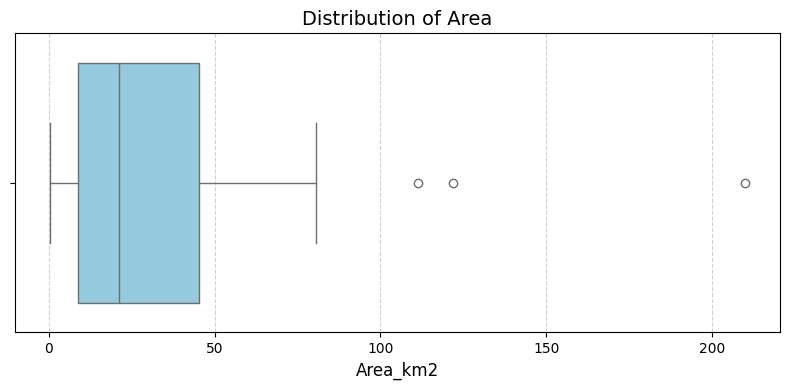
\includegraphics[scale=0.5]{figures/boxplot_area.png}
    \centering
    \caption{'Area\_km2' Feature Boxplot}
    \label{fig:box_area}
\end{figure}

\begin{figure}[!htbp]
    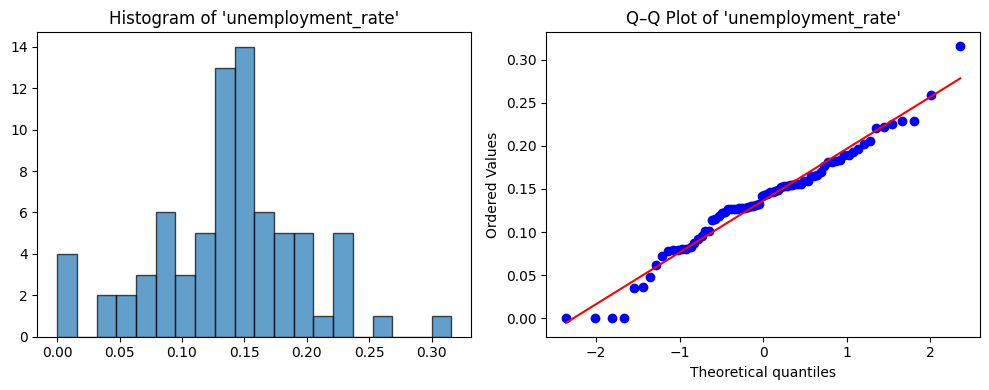
\includegraphics[scale=0.5]{figures/stat_unemployment_rate.png}
    \centering
    \caption{'unemployment\_rate' Feature Histogram \& QQ-Plot}
    \label{fig:stat_unemployment}
\end{figure}

\begin{figure}[!htbp]
    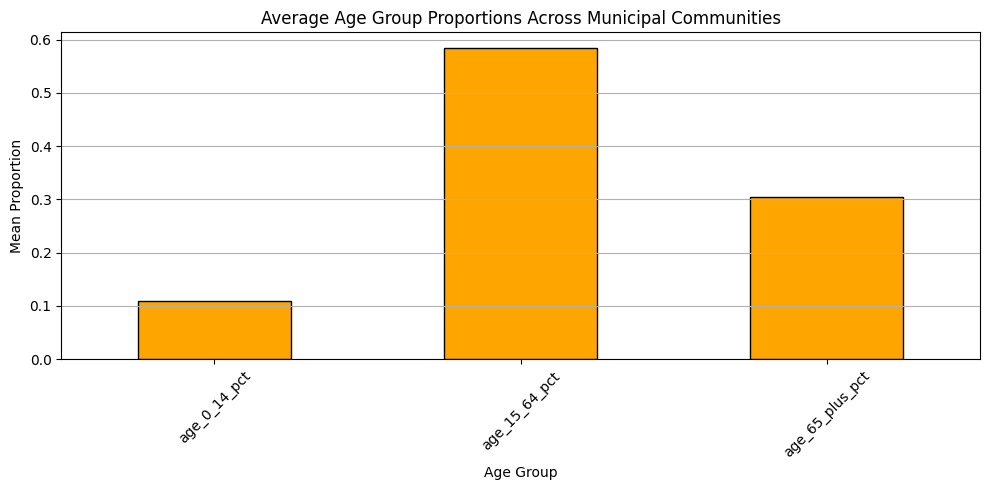
\includegraphics[scale=0.45]{figures/barchart_age_group_means.png}
    \centering
    \caption{Mean Age Group Features Bar Chart}
    \label{fig:bar_age_mean}
\end{figure}

\begin{figure}[!htbp]
    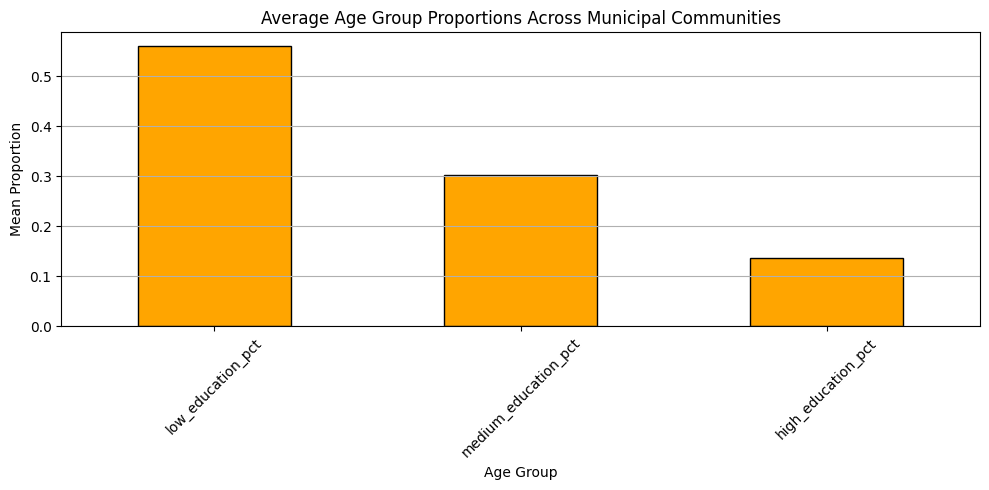
\includegraphics[scale=0.45]{figures/barchart_education_group_means.png}
    \centering
    \caption{Mean Education Group Features Bar Chart}
    \label{fig:bar_education_mean}
\end{figure}

\begin{figure}[!htbp]
    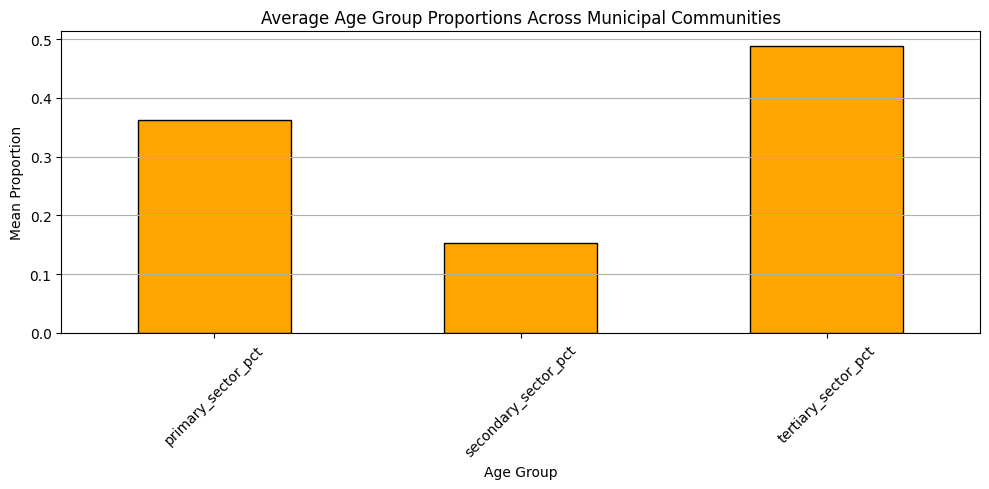
\includegraphics[scale=0.45]{figures/barchart_sector_group_means.png}
    \centering
    \caption{Mean Sector Group Features Bar Chart}
    \label{fig:bar_sector_mean}
\end{figure}


%========================================
\subsubsection{Scatter Plots}

\begin{figure}[h]
    \centering
    \begin{minipage}[b]{0.47\textwidth}
        \centering
        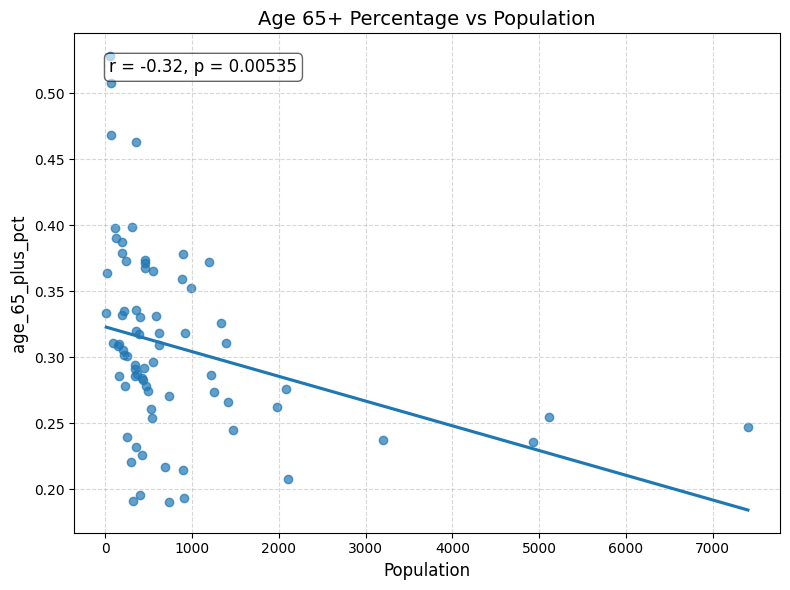
\includegraphics[height=5cm]{figures/scatter_population_elderly.png}
        \caption{Population VS Age 65+}
        \label{fig:scat_pop_elderly}
    \end{minipage}
    \hfill
    \begin{minipage}[b]{0.47\textwidth}
        \centering
        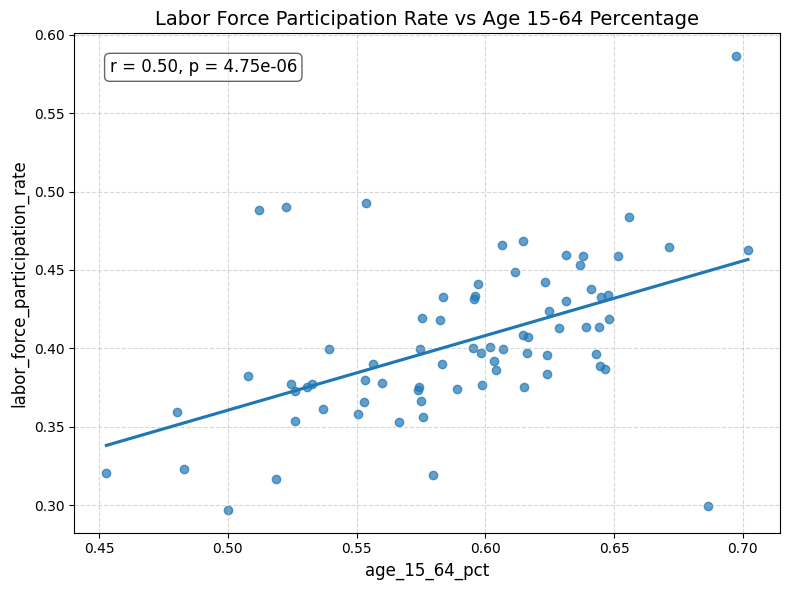
\includegraphics[height=5cm]{figures/scatter_labor_working.png}
        \caption{Labor Force VS Age 15-64 }
        \label{fig:scat_labor_working}
    \end{minipage}
\end{figure}


%========================================
\subsubsection{Correlation Matrices}
\label{sec:correlation_matrices} 

\begin{figure}[!htbp]
    \centering
    \begin{minipage}[b]{0.47\textwidth}
        \centering
        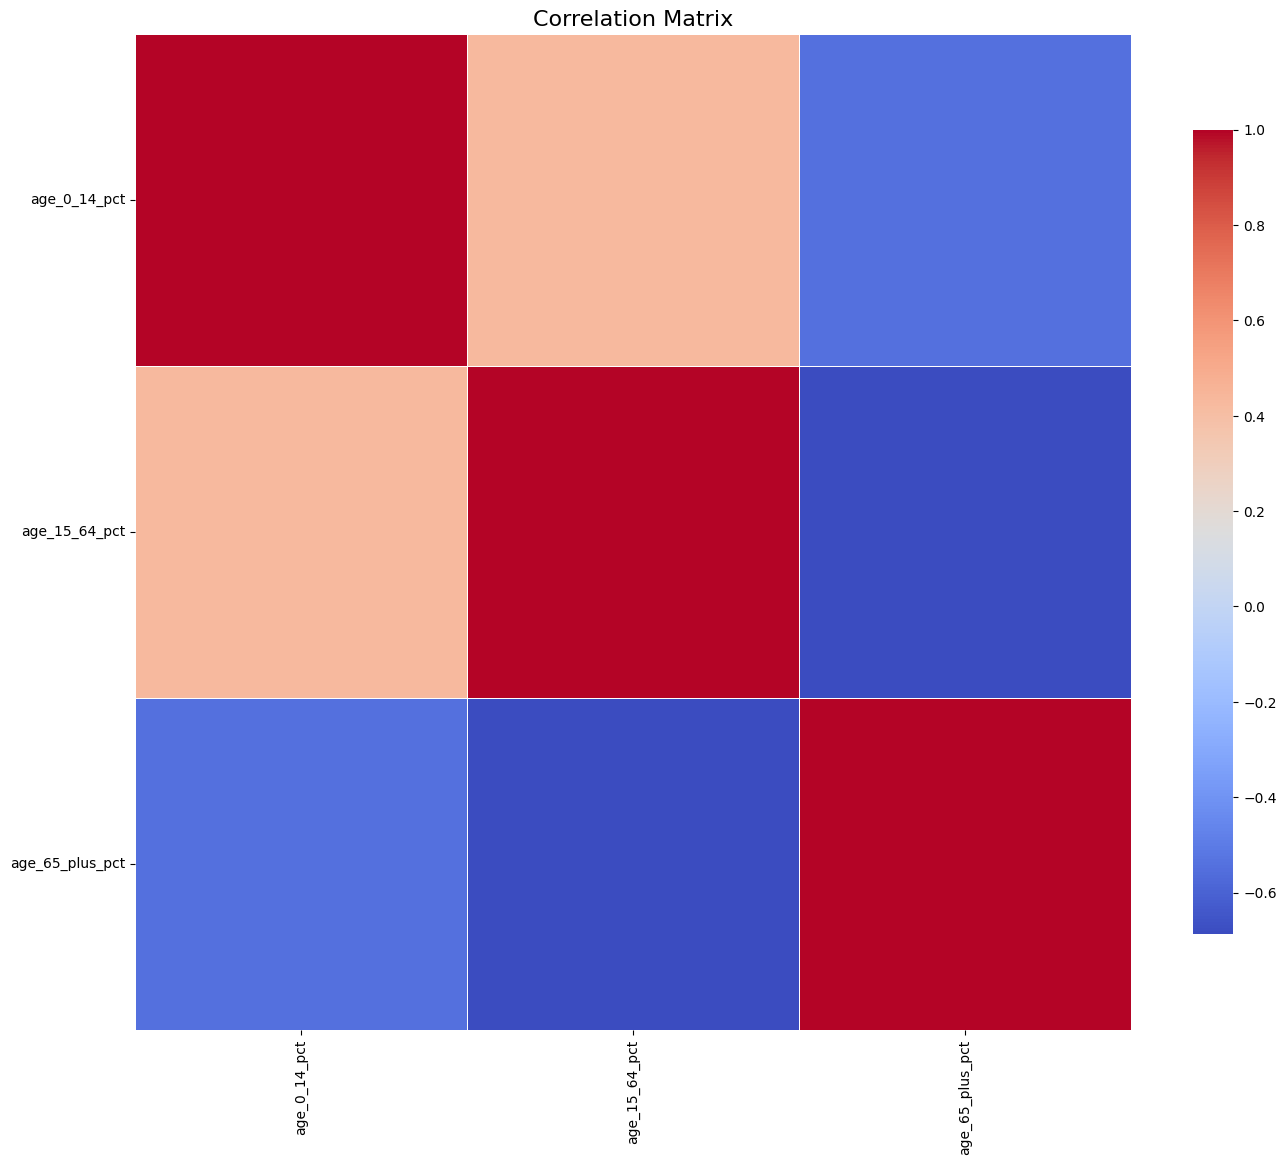
\includegraphics[height=5cm]{figures/corr_age.png}
        \caption{Age Groups}
        \label{fig:corr_age}
    \end{minipage}
    \hfill
    \begin{minipage}[b]{0.47\textwidth}
        \centering
        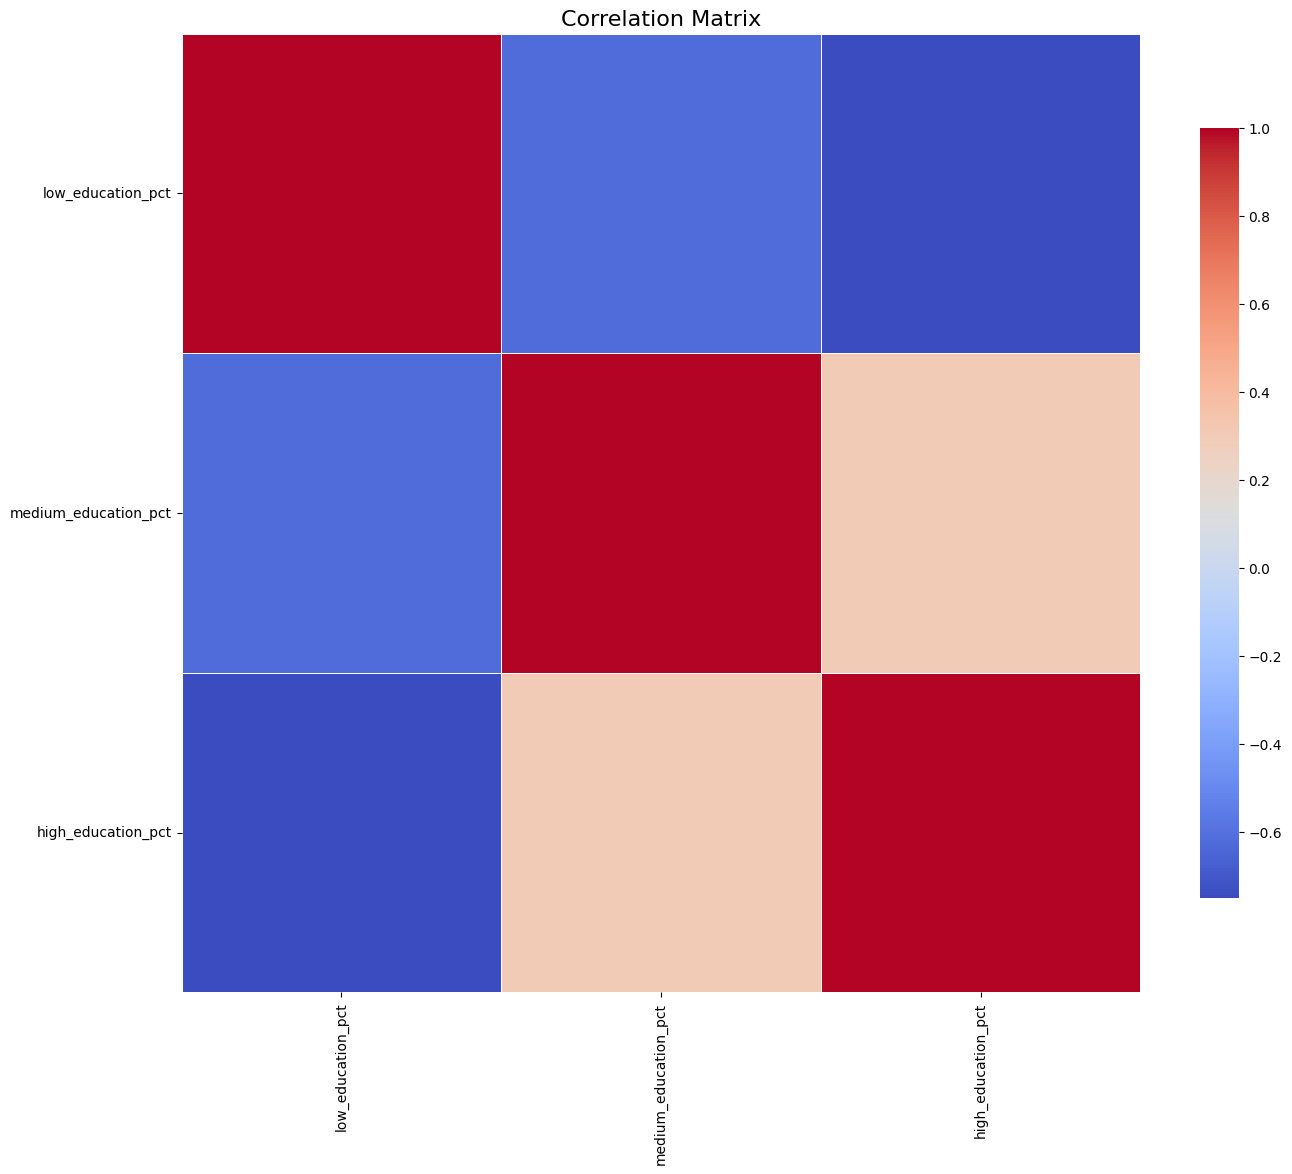
\includegraphics[height=5cm]{figures/corr_education.png}
        \caption{Educational Level Groups}
        \label{fig:corr_education}
    \end{minipage}
\end{figure}

\begin{figure}[!htbp]
    \centering
    \begin{minipage}[b]{0.47\textwidth}
        \centering
        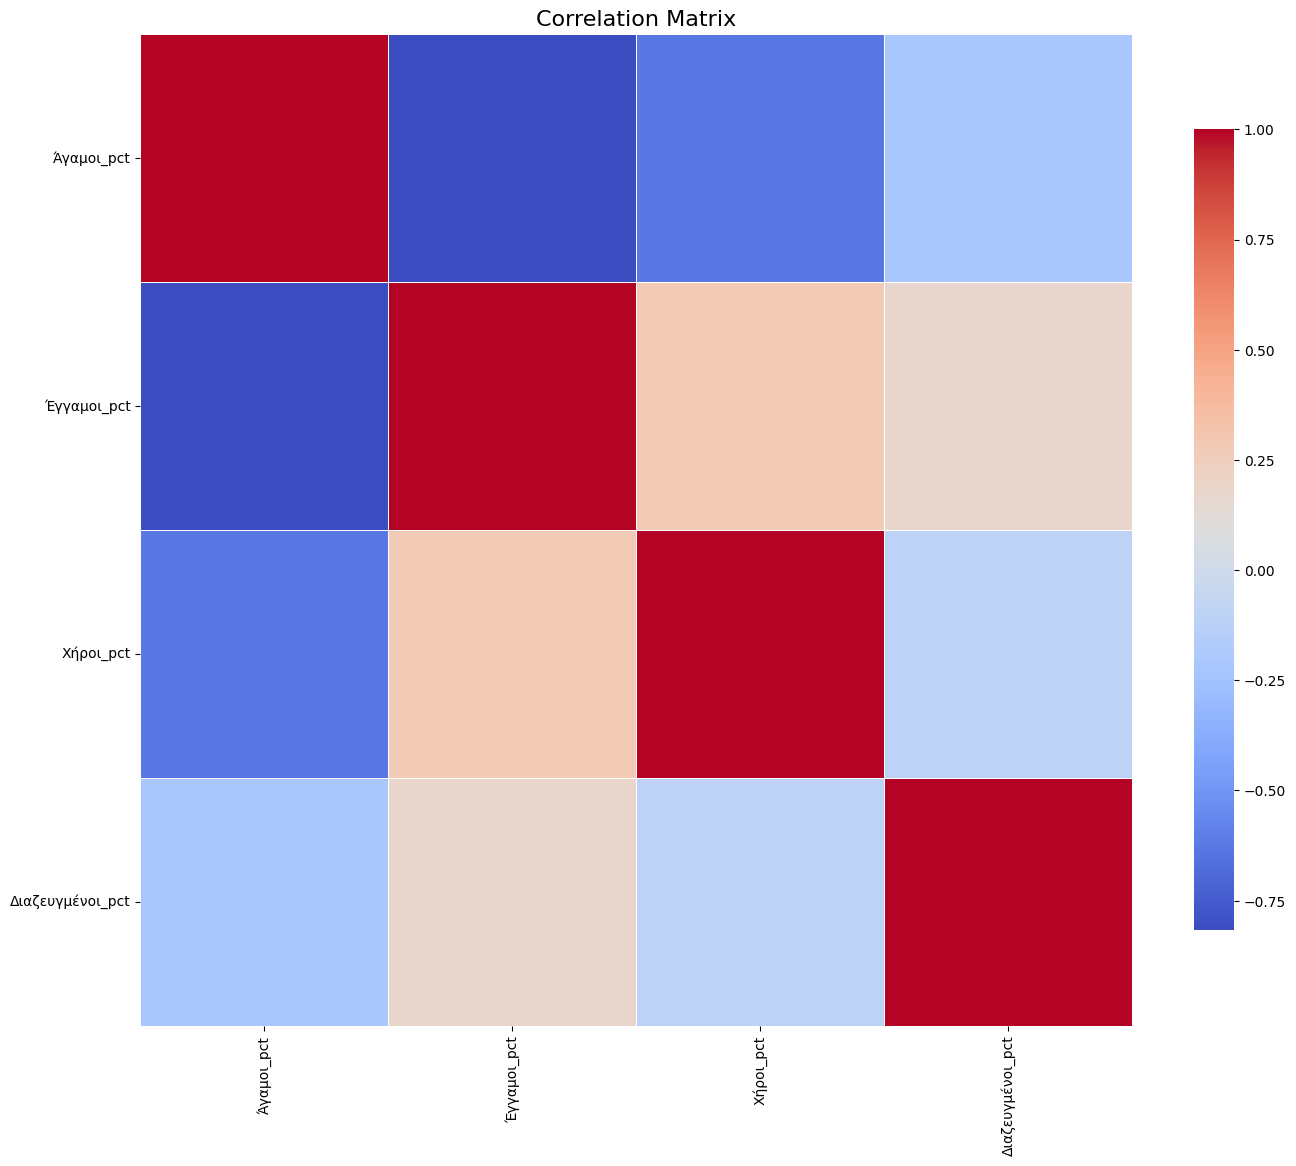
\includegraphics[height=5cm]{figures/corr_marriage.png}
        \caption{Martial Status Groups}
        \label{fig:corr_marriage}
    \end{minipage}
    \hfill
    \begin{minipage}[b]{0.47\textwidth}
        \centering
        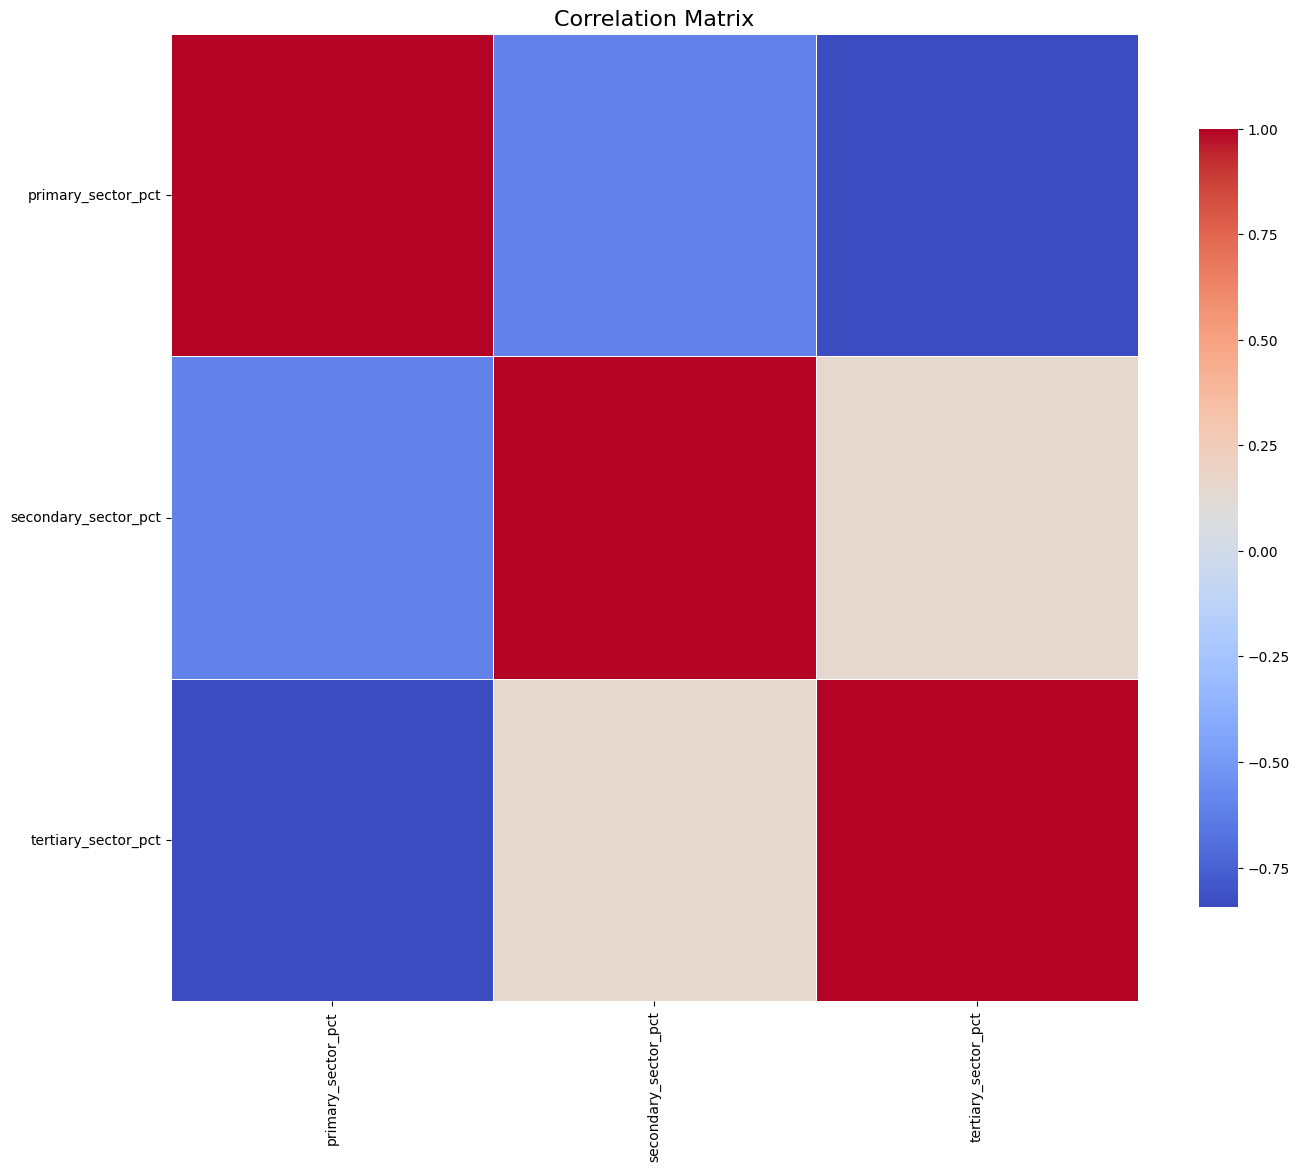
\includegraphics[height=5cm]{figures/corr_sector.png}
        \caption{Sector Groups}
        \label{fig:corr_sector}
    \end{minipage}
\end{figure}


%========================================
\subsubsection{Feature Engineering}
\label{sec:elstat_feature_engineering}

Below is presented the specific modifications performed in the feature groups in order to reduce the dimensionality:

\begin{itemize}
    \item Age Groups: 
        \begin{itemize}
            \item $age\_0\_14\_pct = (0-4)_{\%} + (5-9)_{\%} + (10-14)_{\%}$ (younger people)
            \item $age\_15\_64\_pct = (15-19)_{\%} + (20-24)_{\%} + (25-29)_{\%} + (30-34)_{\%} + (35-39)_{\%} + (40-44)_{\%} + (45-49)_{\%} + (50-54)_{\%} + (55-59)_{\%} + (60-64)_{\%}$ (working people)
            \item $age\_65\_plus\_pct = (65-69)_{\%} + (70-74)_{\%} + (75+)_{\%}$ (elderly people)
        \end{itemize}

    \item Educational Level Groups:
        \begin{itemize}
            \item $low\_education\_pct = no\_formal\_education_{\%} + primary\_education_{\%} + lower\_secondary_{\%}$
            \item $medium\_education\_pct = high\_school_{\%} + post\_secondary\_non\_uni_{\%}$
            \item $high\_education\_pct = higher\_education_{\%}$
        \end{itemize}

    \item Economic Hierarchical Features:
        \begin{itemize}
            \item $unemployment\_rate = \frac{\text{Άνεργοι}}{\text{Οικονομικά ενεργοί}}$
            \item $labor\_force\_participation\_rate = \frac{\text{Οικονομικά ενεργοί}}{\text{Σύνολο}}$
            \item $primary\_sector\_pct = \frac{\text{Πρωτογενής}}{\text{Απασχολούμενοι}}$
            \item $secondary\_sector\_pct = \frac{\text{Δευτερογενής}}{\text{Απασχολούμενοι}}$
            \item $tertiary\_sector\_pct = \frac{\text{Τριτογενής}}{\text{Απασχολούμενοι}}$
        \end{itemize}
\end{itemize}




%========================================
%========================================
%========================================

\section{Neighborhoods Dataset}

This section provides information about the structure of the Neighborhoods Dataset after extracting additional features from QGIS:


%========================================
\subsection{Datasets Structure}

Here we present the structure of the neighborhood dataset. 

\begin{longtable}{p{5cm} p{10cm}}
    \caption{Neighborhood Dataset Columns (highlighted features are used for joining)} \label{tab:neighborhood_columns} \\
    \hline
    \textbf{Column Name} & \textbf{Description} \\
    \hline
    \endfirsthead
    
    \multicolumn{2}{c}{{\bfseries Table \thetable\ (continued)}} \\
    \hline
    \textbf{Column Name} & \textbf{Description} \\
    \hline
    \endhead
    
    \hline \multicolumn{2}{r}{{Continued on next page}} \\
    \endfoot
    
    \hline
    \endlastfoot
    
    Neighborhood\_Greek & Neighborhood name in Greek \\
    Neighborhood & Neighborhood name in English \\
    Centroid\_x & Longitude coordinate of the neighborhood centroid \\
    Centroid\_y & Latitude coordinate of the neighborhood centroid \\
    Neighborhood\_Area\_km2 & Total area of the neighborhood polygon in square kilometers \\
    Geometry & Polygon geometry representing the neighborhood boundary \\
    distance\_to\_volos\_center\_km & Distance from the neighborhood centroid to the Volos city center (km)\\
    distance\_to\_volos\_port\_km & Distance from the neighborhood centroid to the Volos port (km)\\
    dist\_to\_main\_road\_km & Distance from the neighborhood centroid to the nearest main road (km)\\
    dist\_to\_bus\_stop\_km & Distance from the neighborhood centroid to the nearest bus stop (km)\\
    dist\_to\_university\_km & Distance from the neighborhood centroid to the University of Thessaly (km)\\
    \rowcolor{yellow!20}
    Municipal Community & Administrative municipal community in which the neighborhood is located \\
\end{longtable}



%========================================
%========================================
\subsection{Dataset Analysis}

Below we show various visualizations that occured during the EDA of the neighborhood dataset.

%========================================

\subsubsection{Feature Values Distributions}
\FloatBarrier

\begin{figure}[!htbp]
    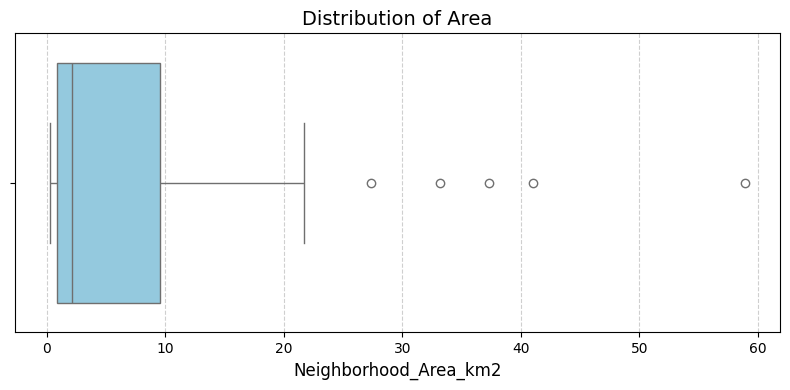
\includegraphics[scale=0.5]{figures/boxplot_area_neighbor.png}
    \centering
    \caption{'Neighborhood\_area\_km2' Feature Boxplot}
    \label{fig:box_area_neigh}
\end{figure}

\begin{figure}[!htbp]
    \centering
    \begin{subfigure}[b]{0.47\textwidth}
        \centering
        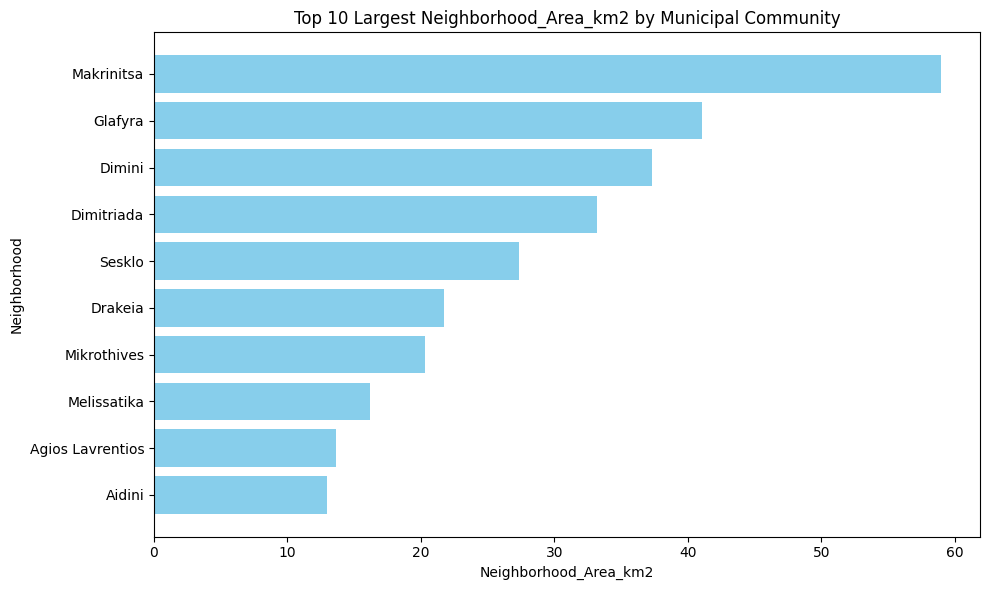
\includegraphics[height=5cm]{figures/barchart_area_neighborhood.png}
        \caption{Neighborhood area Bar Chart}
        \label{fig:bar_area_neigh}
    \end{subfigure}
    \hfill
    \begin{subfigure}[b]{0.47\textwidth}
        \centering
        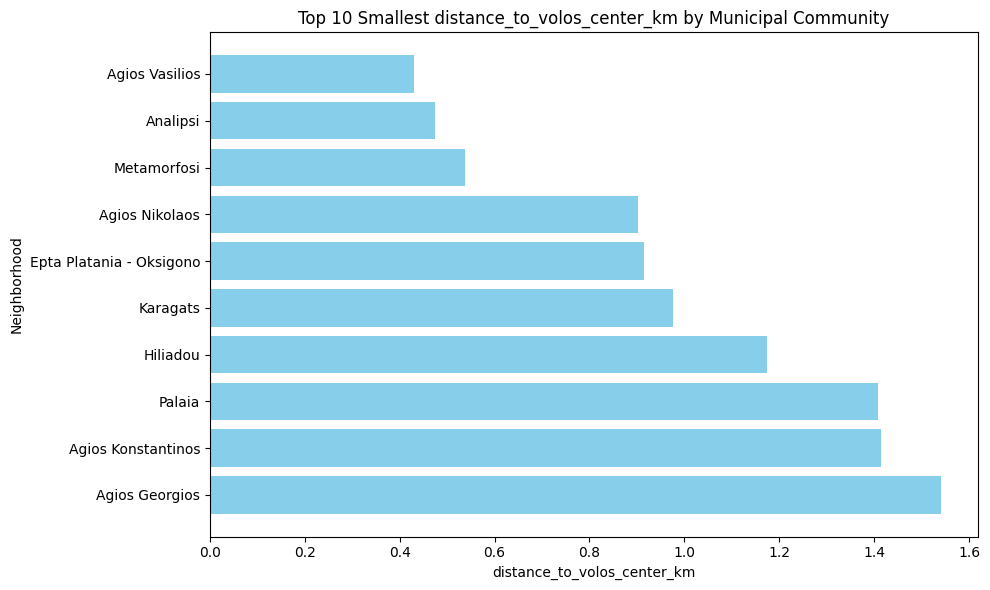
\includegraphics[height=5cm]{figures/barchart_center.png}
        \caption{'Distance to Center  Bar Chart}
        \label{fig:bar_center_neigh}
    \end{subfigure}
\end{figure}

%========================================
\newpage
\subsubsection{Scatter Plots}
\FloatBarrier

\begin{figure}[!htbp]
    \centering
    \begin{subfigure}[b]{0.47\textwidth}
        \centering
        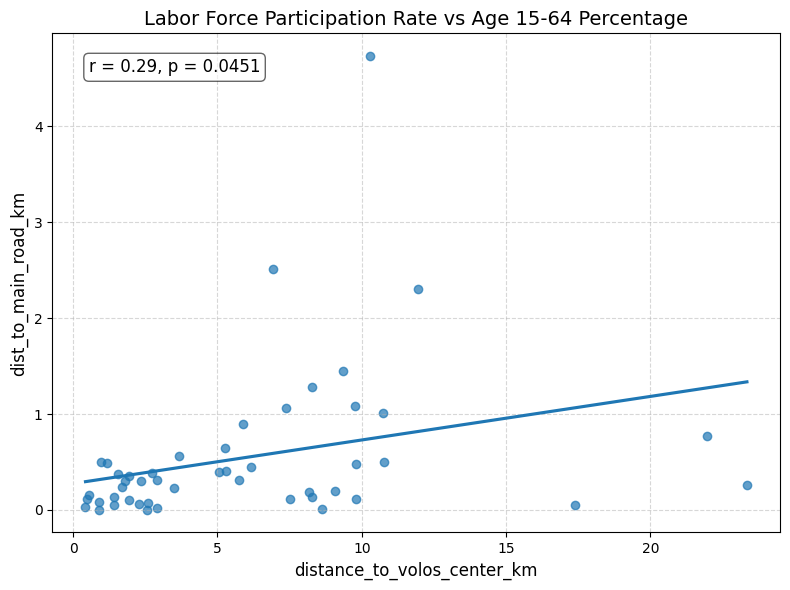
\includegraphics[height=5cm]{figures/scatter_center_highway.png}
        \caption{Distance from Center VS Distance from Main Roads}
        \label{fig:scatter_center_highway}
    \end{subfigure}
    \hfill
    \begin{subfigure}[b]{0.47\textwidth}
        \centering
        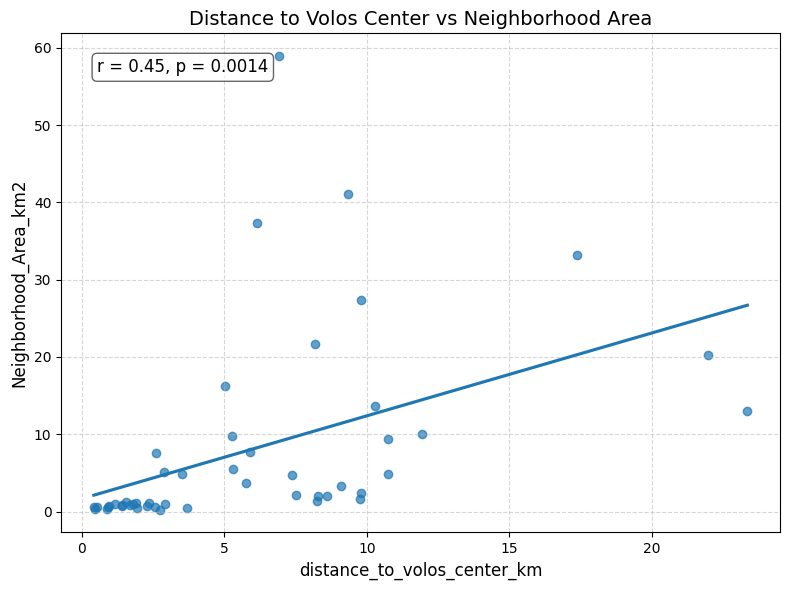
\includegraphics[height=5cm]{figures/scatter_center_area.png}
        \caption{Distance from Center VS Neighborhood Area}
        \label{fig:scatter_center_area}
    \end{subfigure}
\end{figure}





%========================================
%========================================
%========================================
\section{Joined Dataset}

This appendix contains information about the business dataset after joining it both with the neighborhood and municipal community features. 

%========================================
%========================================
\subsection{Dataset Structure}

This section provides the structure of the joined business dataset.

\begin{longtable}{p{5cm} p{10cm}}
    \caption{Joined Dataset Columns} \label{tab:business_joined_columns} \\
    \hline
    \textbf{Column Name} & \textbf{Description} \\
    \hline
    \endfirsthead
    
    \multicolumn{2}{c}{{\bfseries Table \thetable\ (continued)}} \\
    \hline
    \textbf{Column Name} & \textbf{Description} \\
    \hline
    \endhead
    
    \hline \multicolumn{2}{r}{{Continued on next page}} \\
    \endfoot
    
    \hline
    \endlastfoot
    
    Name & Business name as listed in the source dataset \\
    Category & General business category (e.g., restaurant, retail, service) \\
    Latitude & Geographic latitude coordinate of the business location \\
    Longitude & Geographic longitude coordinate of the business location \\
    Address & Full street address of the business \\
    Country & Country where the business is located \\
    City & City where the business is located \\
    Postal Code & Postal code of the business location \\
    Rating & Average rating score given by customers, if available \\
    Reviews & Number of customer reviews, if available \\
    Source & Origin of the business entry \\
    Description & Short textual description of the business \\
    NACE Code & Official NACE classification code for the business activity \\
    NACE Description (EN) & English description of the NACE code activity \\
    Municipal Community & The municipal community of the business location \\
    Neighborhood & The neighborhood of the business location \\
    ΠΕΡΙΦΕΡΕΙΑΚΗ ΕΝΟΤΗΤΑ & Greek regional unit where the business is located \\
    ΔΗΜΟΣ & Municipality where the business is located \\
    ΔΗΜΟΤΙΚΗ ΕΝΟΤΗΤΑ & Municipal unit of the business location \\
    Population & Total population of the municipal community \\
    Άγαμοι\_pct & Percentage of unmarried individuals in the population \\
    Έγγαμοι\_pct & Percentage of married individuals in the population \\
    Χήροι\_pct & Percentage of widowed individuals in the population \\
    Διαζευγμένοι\_pct & Percentage of divorced individuals in the population \\
    age\_0\_14\_pct & Percentage of population aged 0–14 \\
    age\_15\_64\_pct & Percentage of population aged 15–64 \\
    age\_65\_plus\_pct & Percentage of population aged 65 and older \\
    low\_education\_pct & Percentage of population with low education level \\
    medium\_education\_pct & Percentage of population with medium education level \\
    high\_education\_pct & Percentage of population with high education level \\
    unemployment\_rate & Unemployment rate in the municipal community \\
    labor\_force\_participation\_rate & Labor force participation rate in the municipal community \\
    primary\_sector\_pct & Employment percentage in the primary sector\\ 
    secondary\_sector\_pct & Employment percentage in the secondary sector \\
    tertiary\_sector\_pct & Employment percentage in the tertiary sector \\
    Area\_km2 & Total area of the municipal community in square kilometers \\
    Neighborhood\_Area\_km2 & Total area of the neighborhood in square kilometers \\
    distance\_to\_volos\_center\_km & Distance from the neighborhood center to Volos city center (km) \\
    distance\_to\_volos\_port\_km & Distance from the neighborhood center to Volos port (km) \\
    dist\_to\_main\_road\_km & Distance from the neighborhood center to the nearest main road (km) \\
    dist\_to\_bus\_stop\_km & Distance from the neighborhood center to the nearest bus stop (km) \\
    dist\_to\_university\_km & Distance from the neighborhood center to the nearest university (km) \\
\end{longtable}


%========================================
%========================================
\subsection{Missing Data Analysis}

Here we present a heatmap of the missing values across all the features of the joined dataset.

\begin{figure}[h]
    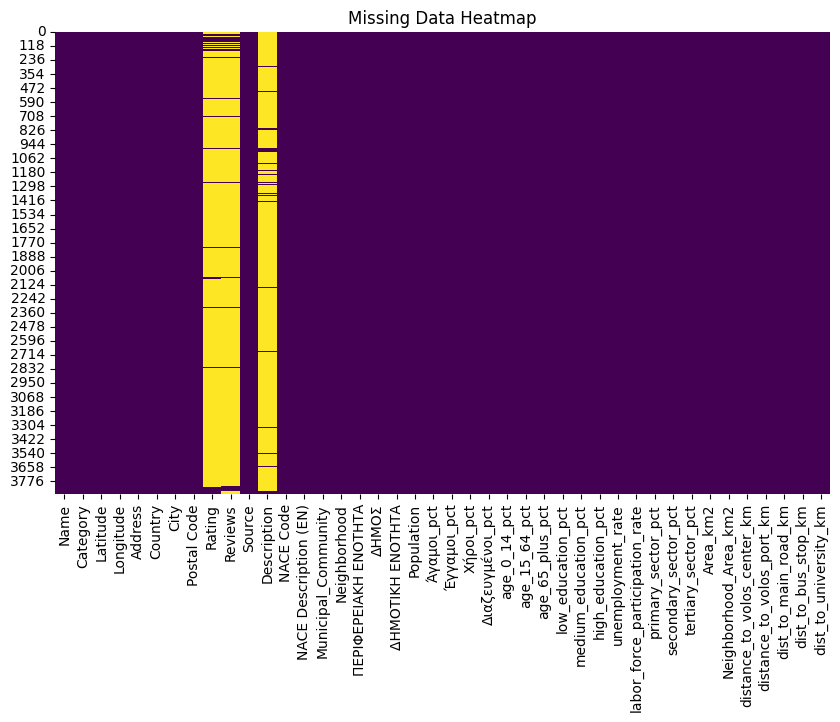
\includegraphics[scale=0.45]{figures/heatmap_missing.png}
    \centering
    \caption{Missing Data Heatmap}
    \label{fig:heatmap_missing}
\end{figure}



%========================================
%========================================
%========================================
\section{Proxy Ground Truths}
\label{venn_diagrams}


This appendix contains information about the procedure of creating the proxy ground truths. Below we present some indicative Venn diagrams of the agreement count between the three different proxy truth creation methods. Not every single one will be shown since their total number is 306 (1 per NACE class).


\begin{figure}[h]
    \centering
    \begin{minipage}[b]{0.47\textwidth}
        \centering
        
\includegraphics[height=5cm]{figures/venn_nace_47_25.png}
        \caption{Venn Diagram for NACE Class 47.25 (Partial Similarity)}
        \label{fig:venn_nace_47_25}
    \end{minipage}
    \hfill
    \begin{minipage}[b]{0.47\textwidth}
        \centering
        
\includegraphics[height=5cm]{figures/venn_nace_28_49.png}
        \caption{Venn Diagram for NACE Class 28.49 (Perfect Similarity)}
        \label{fig:venn_nace_28_49}
    \end{minipage}
\end{figure}



    \renewcommand{\thechapter}{B}
    \chapter{Fine-tuned LLM and Chatbot}

This appendix contains information about the workflow of fine-tuning an LLM to specialize in suggesting optimal business locations, and its transformation to a chatobt application.


%===================================
\section{Fixed Features of Fine-Tuning Dataset}

During the fine-tuning dataset construction, a proportion of the following features will always be selected as justification, regardless of their SHAP importance.

\begin{table}[ht!]
    \centering
    \begin{tabular}{|M{10cm}|}
        \hline
        \textbf{Fixed Features} \\ \hline
        "Neighborhood\_Area\_km2" \\ \hline
        "distance\_to\_volos\_center\_km" \\ \hline
        "distance\_to\_volos\_port\_km" \\ \hline
        "dist\_to\_main\_road\_km" \\ \hline
        "dist\_to\_bus\_stop\_km" \\ \hline
        "dist\_to\_university\_km" \\ \hline
        "Population" \\ \hline
    \end{tabular}
    \caption{Fixed Fine-Tuning Features}
    \label{tab:fixed_features}
\end{table}



%===================================
\section{Training Configuration}

Below, we present the detailed description of the configuration parameters chosen to perform the LLM fine-tuning.

\begin{table}[htbp]
    \centering
    \caption{Fine-tuning configuration of the QLoRA setup.}
    \label{tab:finetune_config}
    \begin{tabular}{ll}
    \hline
    \textbf{Component} & \textbf{Configuration} \\
    \hline
    \multicolumn{2}{l}{\textit{Quantization (bitsandbytes)}} \\
    Weight precision & 4-bit (NF4) \\
    Compute dtype & FP16 \\
    Double quantization & Enabled \\
    Base model & \texttt{mistralai/Mistral-7B-Instruct-v0.2} \\
    \hline
    \multicolumn{2}{l}{\textit{LoRA adapters}} \\
    Rank ($r$) & 16 \\
    Scaling factor ($\alpha$) & 64 \\
    Dropout & 0.05 \\
    Bias & None \\
    Task type & Causal LM \\
    Trainable parameters & $\sim$6.8M ($\approx$0.18\% of total) \\
    \hline
    \multicolumn{2}{l}{\textit{Training arguments}} \\
    Batch size (per device) & 2 \\
    Gradient accumulation & 4 (effective batch size = 8) \\
    Learning rate & 2e-5 \\
    Optimizer & Paged AdamW (32-bit) \\
    LR scheduler & Cosine \\
    Warmup steps & 10 \\
    Epochs & 3 (with further runs at 5 and 8) \\
    Precision & bf16 \\
    Logging steps & 25 \\
    Checkpointing & Save every 100 steps (keep max 2) \\
    Gradient checkpointing & Enabled \\
    \hline
    \end{tabular}
\end{table}



%===================================
\section{Custom CSS \& HTML Messages}

Below, we demonstrate the custom CSS/HTML templates used for the user and assistant messages.

\begin{lstlisting}[language=Python, caption={Rendering User Messages}, label={lst:render_user}]

def render_user_message(message):
    return f"""
    <div style="display: flex; justify-content: flex-end;">
        <div style="background-color:#D2E3FC; border-radius:10px; padding:10px 15px; margin:8px 0; max-width:80%; text-align:left;">
            <b>You:</b><br>{message}
        </div>
    </div>
    """
\end{lstlisting}

\begin{lstlisting}[language=Python, caption={Rendering Assistant Messages}, label={lst:render_assistant}]

def render_assistant_message(message):
    return f"""
    <div style="background-color:#F1F0F0; border-radius:10px; padding:10px 15px; margin:8px 0; width:fit-content; max-width:80%;">
        <b>Assistant:</b><br>{message}
    </div>
    """
\end{lstlisting}


    \renewcommand{\thechapter}{C}
    \chapter{Evaluation of Approaches}

This appendix contains information about the evaluation of the two approaches. We show analytically the calculated metric values.


%===================================
\section{Fine-Tuned LLM Results}

The following table demonstrates the calculated values of the evaluation metrics for the fine-tuned LLM approach.


\begin{table}[h!]
    \centering
    \caption{Evaluation metrics across different training epochs}
    \label{tab:results_ft}
    \resizebox{\textwidth}{!}{%
    \begin{tabular}{lcccccc}
    \hline
    \textbf{Epochs} & \textbf{BERT Precision} & \textbf{BERT Recall} & \textbf{BERT F1} & \textbf{Match@3} & \textbf{Precision@3} & \textbf{Recall@3} \\
    \hline
    3 Epochs & 0.9229 & 0.9133 & 0.9181 & 0.7862 & 0.3145 & 0.3145 \\
    5 Epochs & 0.9228 & 0.9202 & 0.9215 & 0.7799 & 0.3187 & 0.3187 \\
    8 Epochs & 0.9188 & 0.9179 & 0.9183 & 0.6981 & 0.2851 & 0.2851 \\
    \hline
    \end{tabular}%
    }
\end{table}



%===================================
\section{RAG Pipeline Results}

The following table demonstrates the calculated values of the evaluation metrics for the RAG pipeline approach.

\begin{table}[h!]
    \centering
    \caption{Evaluation metrics across different approaches}
    \label{tab:results_rag}
    \resizebox{\textwidth}{!}{%
    \begin{tabular}{lcccccc}
    \hline
    \textbf{Attempts} & \textbf{BERT Precision} & \textbf{BERT Recall} & \textbf{BERT F1} & \textbf{Match@3} & \textbf{Precision@3} & \textbf{Recall@3} \\
    \hline
    10 Justifications & 0.8727 & 0.8381 & 0.8550 & 0.8302 & 0.3669 & 0.3669 \\
    15 Justifications & 0.8648 & 0.8314 & 0.8477 & 0.7862 & 0.3548 & 0.3522 \\
    20 Justifications & 0.8608 & 0.8290 & 0.8446 & 0.7107 & 0.2778 & 0.2893 \\
    \hline
    \end{tabular}%
    }
\end{table}


%===================================
\section{Approaches Comparison}

The following table demonstrates the calculated values of the evaluation metrics for the fine-tuned LLM and RAG pipeline approaches. The best attempt of each system is selected. 


%===================================
\subsection{Semantic \& Recommendation Metrics}

Below we compare the metrics that measure semantic similarity and recommendation accuracy.

\begin{table}[h!]
    \centering
    \caption{Semantic \& Recommendation Metrics across both Approaches}
    \label{tab:results_ft_rag}
    \resizebox{\textwidth}{!}{%
    \begin{tabular}{lcccccc}
    \hline
    \textbf{Approach} & \textbf{BERT Precision} & \textbf{BERT Recall} & \textbf{BERT F1} & \textbf{Match@3} & \textbf{Precision@3} & \textbf{Recall@3} \\
    \hline
    Fine-Tuned LLM & 0.9228 & 0.9202 & 0.9215 & 0.7799 & 0.3187 & 0.3187 \\
    RAG Pipeline & 0.8727 & 0.8381 & 0.8550 & 0.8302 & 0.3669 & 0.3669 \\
    \hline
    \end{tabular}%
    }
\end{table}

%===================================
\subsection{Efficiency Metrics}

Below, we compare the metrics that measure the runtime duration of each approach.

\begin{table}[h!]
    \centering
    \caption{Efficiency Metrics across both Approaches}
    \label{tab:results_ft_rag_time}
    \begin{tabular}{lcc}
    \hline
    \textbf{Approach} & \textbf{Average Time per Query (s)} & \textbf{Total Runtime (mm:ss)} \\
    \hline
    Fine-Tuned LLM & 16.00 & 12:31 \\
    RAG Pipeline   & 37.56 & 42:24 \\
    \hline
    \end{tabular}
\end{table}


%===================================
\subsection{Strengths and Limitations}

Below, we provide a table that analytically describes the advantages and disadvantages of the two frameworks. 


\begin{longtable}{>{\bfseries}p{0.20\textwidth} Y Y}
    \caption{Fine-tuned LLM vs.\ RAG with Re-Ranking} \\
    \label{tab:comparison_ft_rag}
    \toprule
    Aspect & Fine-tuned LLM & RAG with Re-Ranking Pipeline \\
    \midrule
    \endfirsthead
    
    \toprule
    Aspect & Fine-tuned LLM & RAG with Re-Ranking Pipeline \\
    \midrule
    \endhead
    
    \midrule
    \multicolumn{3}{r}{\emph{Continued on next page}} \\
    \midrule
    \endfoot
    
    \bottomrule
    \endlastfoot
    
    Core Idea
    & Train an LLM (Mistral-7B-Instruct with QLoRA) to directly generate top-3 business location recommendations with justifications.
    & Use embeddings to retrieve relevant neighborhoods and re-rank based on similarity to the user query; LLM (Llama 3) only formats the final output. \\
    
    Strengths
    & \begin{itemize}[leftmargin=*, nosep]
        \item Fast inference after training (if GPU is utilized)
        \item Learns domain-specific patterns
        \item Can generalize to unseen but similar prompts
      \end{itemize}
    & \begin{itemize}[leftmargin=*, nosep]
        \item Dynamic: no need to retrain when data updates
        \item Reduces hallucinations (data fetched at runtime)
        \item Easier to personalize results to user preferences
      \end{itemize} \\
    
    Limitations
    & \begin{itemize}[leftmargin=*, nosep]
        \item Static: retraining required for new NACE classes or updated proxy truths
        \item Risk of hallucination in justifications
        \item High initial computational cost
        \item One-to-one conversation does not fully utilize the GPU
      \end{itemize}
    & \begin{itemize}[leftmargin=*, nosep]
        \item Slower inference (retrieval {+} embedding overhead)
        \item Dependent on embedding quality
        \item Requires additional infrastructure (vector DB / storage)
      \end{itemize} \\
    
    Explainability
    & Built-in through feature \& neighborhood justification (SHAP {+} percentile templates).
    & Explainability derived from neighborhood descriptions (feature statistics \& contextual text). \\
    
    Adaptability
    & Less flexible -- retraining needed when data or categories change.
    & Highly flexible -- can add new businesses, neighborhoods, or user constraints without retraining. \\
    
    Computational Resources
    & Requires HPC (A100 GPU) for fine-tuning; optimized via QLoRA (0.18\% trainable params).
    & Moderate GPU/CPU needed for embeddings and inference; feasible to run locally (quantized models). \\
    
    Personalization
    & Limited -- produces 3 static recommendations per NACE class.
    & Strong -- query-specific re-ranking allows user-tailored recommendations. \\
    
    Best Use Case
    & When fast inference on fixed, stable data with concurrent queries or batched workloads is needed, and compute resources are available.
    & When frequent updates, user-specific preferences, and reduced hallucinations are priorities. \\
    
\end{longtable}




    % \renewcommand{\thechapter}{D}
    % \include{appendix_D}

    % \renewcommand{\thechapter}{E}
    % \include{appendix_E}

% Εάν υπάρχει μόνο ένα Παράρτημα,
% μπαίνουν σε σχόλια οι παραπάνω γραμμές 
% και ρυθμίζεται αρίθμηση χωρίς γράμμα
  \renewcommand{\thechapter}{} 
  \renewcommand{\thesection}{\arabic{section}}
%
% Ακολουθεί αρχείο μεμονωμένου Παραρτήματος
% (διαφορετική δομή από appA/appΒ)
%  % Παράρτημα A

\chapter{Datasets Structure \& Analysis}


%========================================
%========================================
%========================================
\section{Business Entries Dataset}

This appendix contains information about the business dataset after unifying the entries from multiple sources, filling the missing values, and adding the NACE code:

%========================================
%========================================
\subsection{Dataset Structure}

This section provides the structure of the pure business dataset (before joining).

\begin{longtable}{p{5cm} p{10cm}}
    \caption{Business Dataset Columns (highlighted features are used for joining)} \label{tab:business_columns} \\
    \hline
    \textbf{Column Name} & \textbf{Description} \\
    \hline
    \endfirsthead
    
    \multicolumn{2}{c}{{\bfseries Table \thetable\ (continued)}} \\
    \hline
    \textbf{Column Name} & \textbf{Description} \\
    \hline
    \endhead
    
    \hline \multicolumn{2}{r}{{Continued on next page}} \\
    \endfoot
    
    \hline
    \endlastfoot
    
    Name & Business name as listed in the source dataset \\
    Category & General business category (e.g., restaurant, retail, service) \\
    Latitude & Geographic latitude coordinate of the business location \\
    Longitude & Geographic longitude coordinate of the business location \\
    Address & Full street address of the business \\
    Country & Country where the business is located \\
    City & City where the business is located \\
    Postal Code & Postal code of the business location \\
    Rating & Average rating score given by customers, if available \\
    Reviews & Number of customer reviews, if available \\
    Source & Origin of the business entry \\
    Description & Short textual description of the business \\
    NACE Code & Official NACE classification code for the business activity \\
    NACE Description (EN) & English description of the NACE code activity \\
    \rowcolor{yellow!20}
    Municipal Community & The municipal community of the business location\\
    \rowcolor{yellow!20}
    Neighborhood & The neighborhood of the business location\\
    
\end{longtable}

%========================================
%========================================
\subsection{Dataset Analysis}


\subsubsection{Feature Values Distributions}

Here we see the most frequent values of the business dataset features that were not explicitly mentioned in the paragraph \ref{EDA_business}.

\begin{figure}[h]
    \centering
    \begin{minipage}[b]{0.45\textwidth}
        \centering
        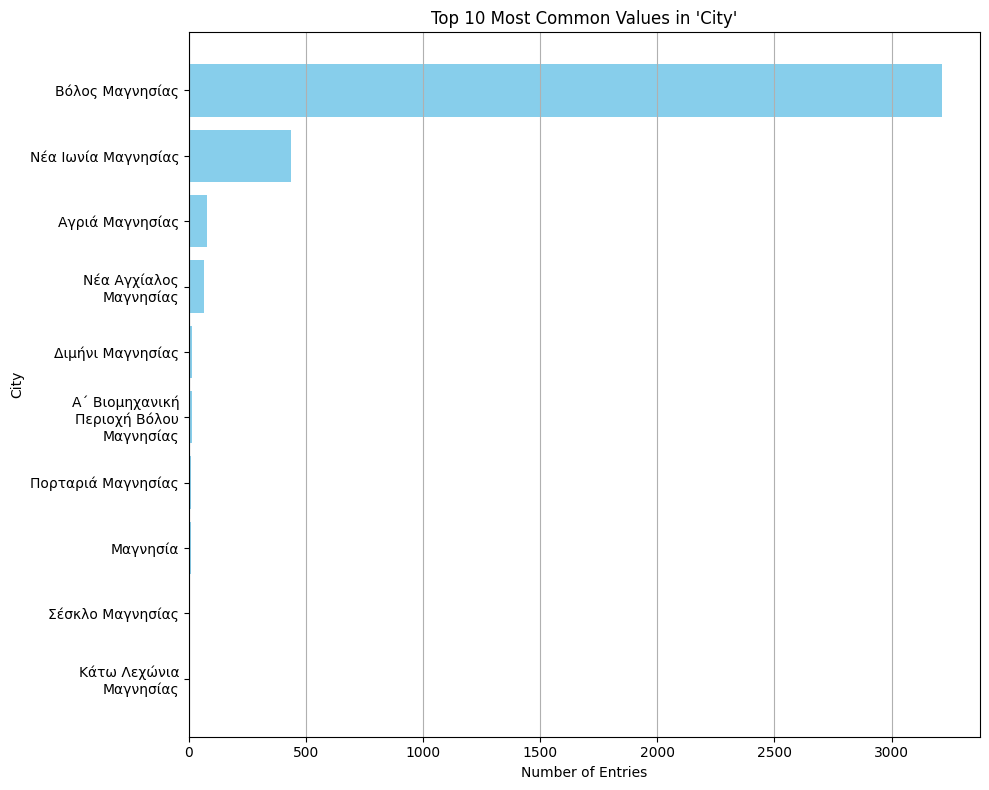
\includegraphics[height=5cm]{figures/distribution_city.png}
        \caption{'City' Bar Chart}
        \label{fig:city_distr}
    \end{minipage}
    \hfill
    \begin{minipage}[b]{0.45\textwidth}
        \centering
        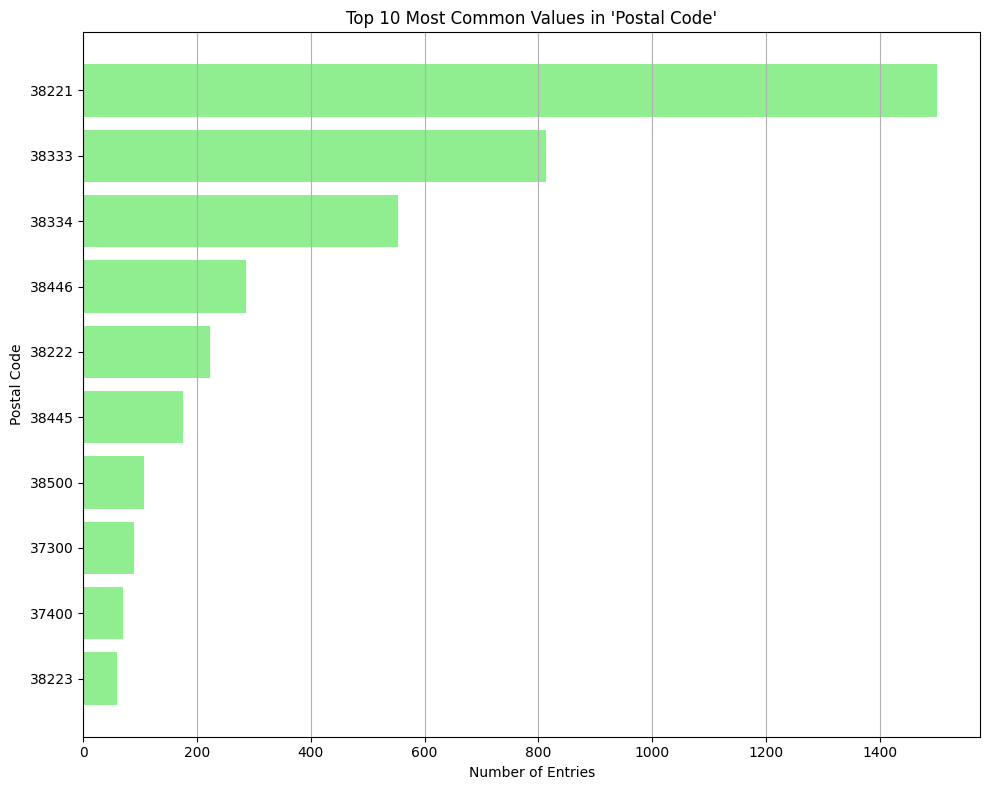
\includegraphics[height=5cm]{figures/distribution_postal_code.png}
        \caption{'Postal Code' Bar Chart}
        \label{fig:postal_distr}
    \end{minipage}
\end{figure}

\begin{figure}[h]
    \centering
    \begin{minipage}[b]{0.45\textwidth}
        \centering
        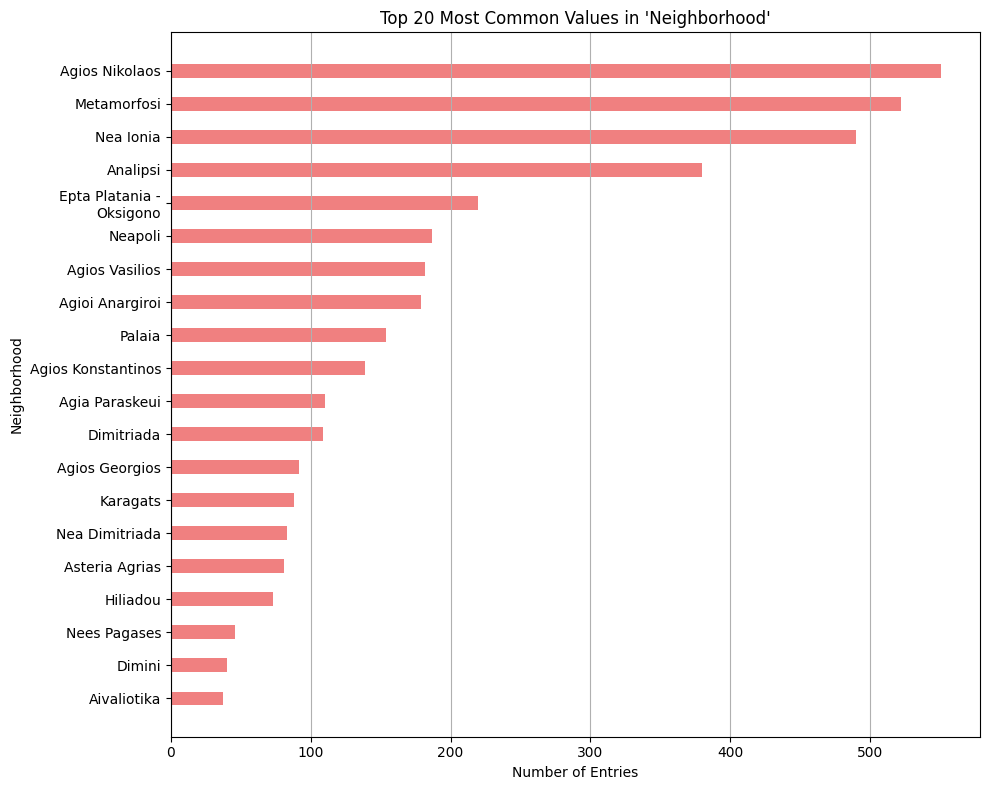
\includegraphics[height=5cm]{figures/distribution_neighborhoods.png}
        \caption{'Neighborhood' Bar Chart}
        \label{fig:neighborhood_distr}
    \end{minipage}
    \hfill
    \begin{minipage}[b]{0.45\textwidth}
        \centering
        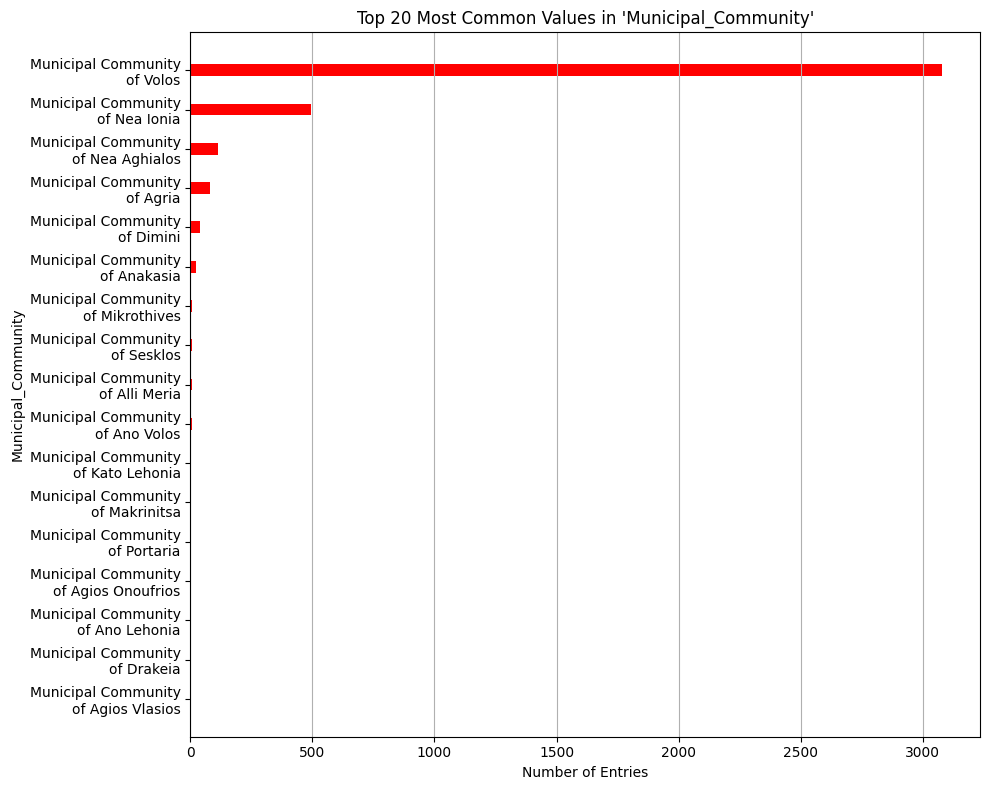
\includegraphics[height=5cm]{figures/distribution_mc.png}
        \caption{'MC' Bar Chart}
        \label{fig:mc_distr}
    \end{minipage}
\end{figure}

\begin{figure}[h]
    \centering
    \begin{minipage}[b]{0.45\textwidth}
        \centering
        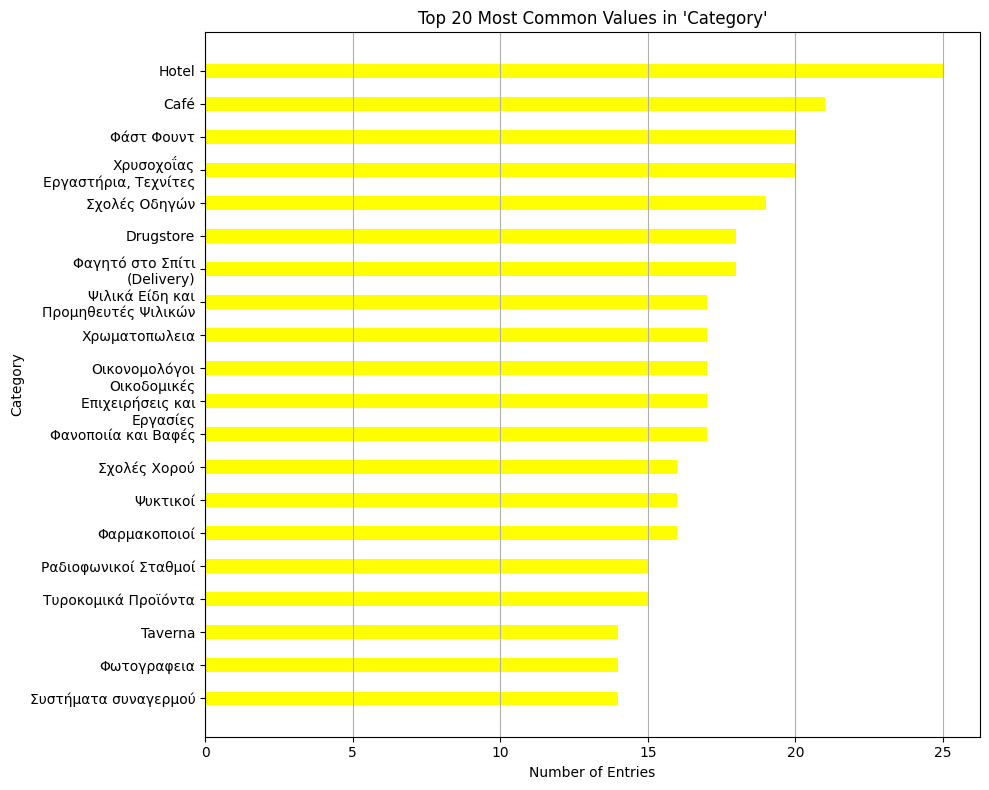
\includegraphics[height=5cm]{figures/distribution_category.png}
        \caption{'Category' Bar Chart}
        \label{fig:category_distr}
    \end{minipage}
    \hfill
    \begin{minipage}[b]{0.45\textwidth}
        \centering
        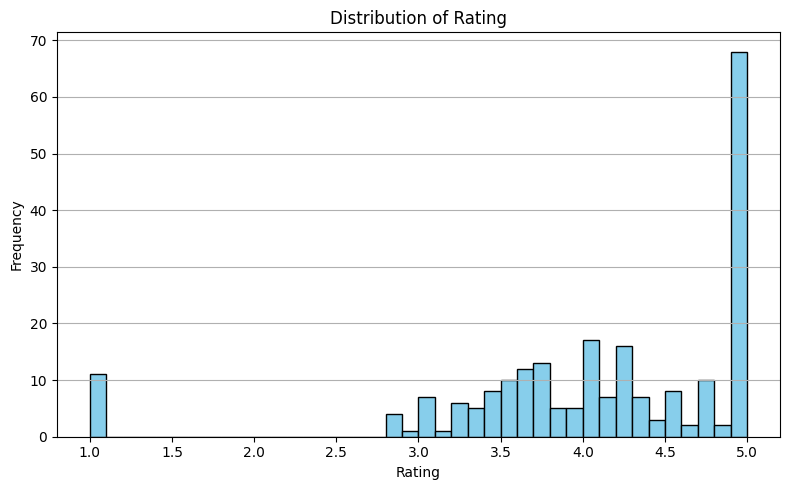
\includegraphics[height=5cm]{figures/distribution_rating.png}
        \caption{'Rating' Histogram}
        \label{fig:distr_rating}
    \end{minipage}
\end{figure}



%========================================
%========================================
%========================================
\newpage
\section{ELSTAT Datasets}

This appendix contains information about the data extracted from the ELSTAT platform: their raw structure, visualizations about their analysis, and more.

%========================================
%========================================
\subsection{Datasets Structure}

Here we present the complete structure of the raw demographic and economic data extracted from the ELSTAT platform.


%========================================
\subsubsection{Raw Demographic Data}

\begin{longtable}{p{5cm} p{10cm}}
    \caption{Demographic Dataset Columns} \label{tab:demographic_columns} \\
    \hline
    \textbf{Column Name} & \textbf{Description} \\
    \hline
    \endfirsthead
    
    \multicolumn{2}{c}{{\bfseries Table \thetable\ (continued)}} \\
    \hline
    \textbf{Column Name} & \textbf{Description} \\
    \hline
    \endhead
    
    \hline \multicolumn{2}{r}{{Continued on next page}} \\
    \endfoot
    
    \hline
    \endlastfoot
    
    ΠΕΡΙΦΕΡΕΙΑΚΗ ΕΝΟΤΗΤΑ & Administrative regional unit where the municipal community belongs \\
    ΔΗΜΟΣ & Municipality name \\
    ΔΗΜΟΤΙΚΗ ΕΝΟΤΗΤΑ & Administrative municipal unit \\
    ΔΗΜΟΤΙΚΗ ΚΟΙΝΟΤΗΤΑ & Administrative municipal community name (Greek) \\
    Population & Total population count \\
    0-4 & Population aged 0 to 4 years \\
    5-9 & Population aged 5 to 9 years \\
    10-14 & Population aged 10 to 14 years \\
    15-19 & Population aged 15 to 19 years \\
    20-24 & Population aged 20 to 24 years \\
    25-29 & Population aged 25 to 29 years \\
    30-34 & Population aged 30 to 34 years \\
    35-39 & Population aged 35 to 39 years \\
    40-44 & Population aged 40 to 44 years \\
    45-49 & Population aged 45 to 49 years \\
    50-54 & Population aged 50 to 54 years \\
    55-59 & Population aged 55 to 59 years \\
    60-64 & Population aged 60 to 64 years \\
    65-69 & Population aged 65 to 69 years \\
    70-74 & Population aged 70 to 74 years \\
    75+ & Population aged 75 years and older \\
    higher\_education & Individuals with higher education (university or equivalent) \\
    post\_secondary\_non\_uni & Individuals with post-secondary non-university education \\
    high\_school & Individuals with completed high school education \\
    lower\_secondary & Individuals with completed lower secondary education \\
    primary\_education & Individuals with completed primary education \\
    no\_formal\_education & Individuals with no formal education \\
    not\_classified & Individuals whose education level is not classified \\
    Άγαμοι & Individuals who are unmarried \\
    Έγγαμοι & Individuals who are married \\
    Χήροι & Individuals who are widowed \\
    Διαζευγμένοι & Individuals who are divorced \\
\end{longtable}


%========================================
\newpage
\subsubsection{Raw Economic Data}

\begin{longtable}{p{5cm} p{10cm}}
    \caption{Economic Dataset Columns} \label{tab:economic_columns} \\
    \hline
    \textbf{Column Name} & \textbf{Description} \\
    \hline
    \endfirsthead
    
    \multicolumn{2}{c}{{\bfseries Table \thetable\ (continued)}} \\
    \hline
    \textbf{Column Name} & \textbf{Description} \\
    \hline
    \endhead
    
    \hline \multicolumn{2}{r}{{Continued on next page}} \\
    \endfoot
    
    \hline
    \endlastfoot
    
    ΠΕΡΙΦΕΡΕΙΑΚΗ ΕΝΟΤΗΤΑ & Administrative regional unit where the municipal community belongs \\
    ΔΗΜΟΣ & Municipality name \\
    ΔΗΜΟΤΙΚΗ ΕΝΟΤΗΤΑ & Administrative municipal unit \\
    ΔΗΜΟΤΙΚΗ ΚΟΙΝΟΤΗΤΑ & Administrative municipal community name (Greek) \\
    Σύνολο & Total reference population for the economic activity statistics \\
    Οικονομικά ενεργοί & Economically active population (employed + unemployed individuals) \\
    Απασχολούμενοι & Employed individuals within the economically active population \\
    Πρωτογενής & Number of employed individuals in the primary economic sector \\
    Δευτερογενής & Number of employed individuals in the secondary economic sector \\
    Τριτογενής & Number of employed individuals in the tertiary economic sector \\
    Άνεργοι & Unemployed individuals within the economically active population \\
    Οικονομικά μη ενεργοί & Economically inactive population (students, retirees, homemakers, etc.) \\
\end{longtable}


%========================================
\newpage
\subsubsection{Processed Demographic \& Economic Data}

\begin{longtable}{p{5cm} p{10cm}}
    \caption{Processed Demographic \& Economic Dataset Columns} \label{tab:final_municipal_communities_columns} \\
    \hline
    \textbf{Column Name} & \textbf{Description} \\
    \hline
    \endfirsthead
    
    \multicolumn{2}{c}{{\bfseries Table \thetable\ (continued)}} \\
    \hline
    \textbf{Column Name} & \textbf{Description} \\
    \hline
    \endhead
    
    \hline \multicolumn{2}{r}{{Continued on next page}} \\
    \endfoot
    
    \hline
    \endlastfoot
    
    ΠΕΡΙΦΕΡΕΙΑΚΗ ΕΝΟΤΗΤΑ & Administrative regional unit where the municipal community belongs \\
    ΔΗΜΟΣ & Municipality name \\
    ΔΗΜΟΤΙΚΗ ΕΝΟΤΗΤΑ & Administrative municipal unit \\
    ΔΗΜΟΤΙΚΗ ΚΟΙΝΟΤΗΤΑ ΕΛΛ & Municipal community name in Greek \\
    ΔΗΜΟΤΙΚΗ ΚΟΙΝΟΤΗΤΑ & Municipal community name in English \\
    Population & Total population count \\
    Άγαμοι\_pct & Percentage of unmarried individuals \\
    Έγγαμοι\_pct & Percentage of married individuals \\
    Χήροι\_pct & Percentage of widowed individuals \\
    Διαζευγμένοι\_pct & Percentage of divorced individuals \\
    age\_0\_14\_pct & Percentage of population aged 0–14 years \\
    age\_15\_64\_pct & Percentage of population aged 15–64 years \\
    age\_65\_plus\_pct & Percentage of population aged 65 years and older \\
    low\_education\_pct & Percentage of population with no formal, primary, or lower secondary education \\
    medium\_education\_pct & Percentage of population with upper secondary or post-secondary non-university education \\
    high\_education\_pct & Percentage of population with higher education (university or equivalent) \\
    unemployment\_rate & Ratio of unemployed individuals to economically active population \\
    labor\_force\_participation\_rate & Ratio of economically active population to total population \\
    primary\_sector\_pct & Percentage of employed individuals in the primary sector \\
    secondary\_sector\_pct & Percentage of employed individuals in the secondary sector \\
    tertiary\_sector\_pct & Percentage of employed individuals in the tertiary sector \\
    Area\_km2 & Area of the municipal community in square kilometers \\
\end{longtable}


%========================================
%========================================
\subsection{Datasets Analysis}


Here, we present the visualizations provided by analyzing the demographic and economic data gathered from the ELSTAT platform. The results of these inspections led to the chosen transformation methods applied in order to prepare the data for later use.


%========================================
\subsubsection{Feature Values Distributions}

Below, we see the most frequent values of the ELSTAT dataset features that were not explicitly mentioned in the paragraph \ref{EDA_mc}.


\begin{figure}[!htbp]
    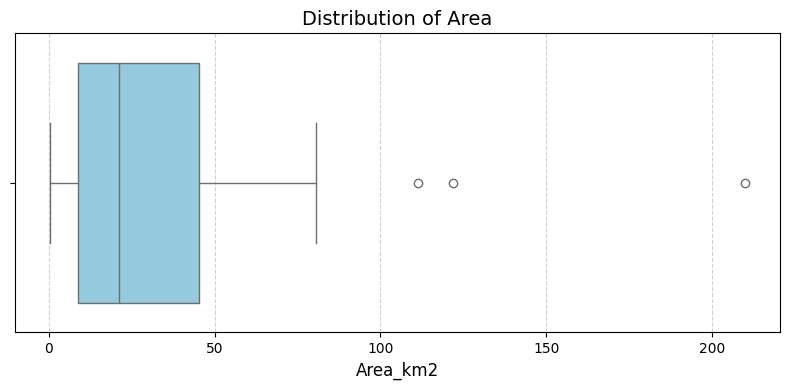
\includegraphics[scale=0.5]{figures/boxplot_area.png}
    \centering
    \caption{'Area\_km2' Feature Boxplot}
    \label{fig:box_area}
\end{figure}

\begin{figure}[!htbp]
    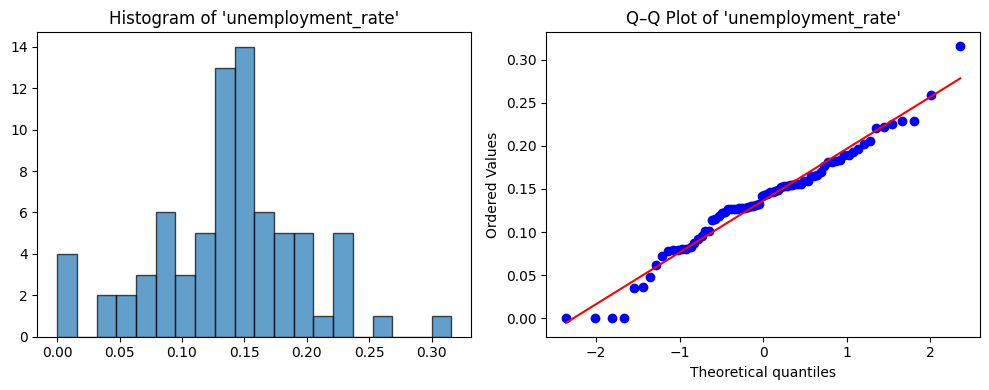
\includegraphics[scale=0.5]{figures/stat_unemployment_rate.png}
    \centering
    \caption{'unemployment\_rate' Feature Histogram \& QQ-Plot}
    \label{fig:stat_unemployment}
\end{figure}

\begin{figure}[!htbp]
    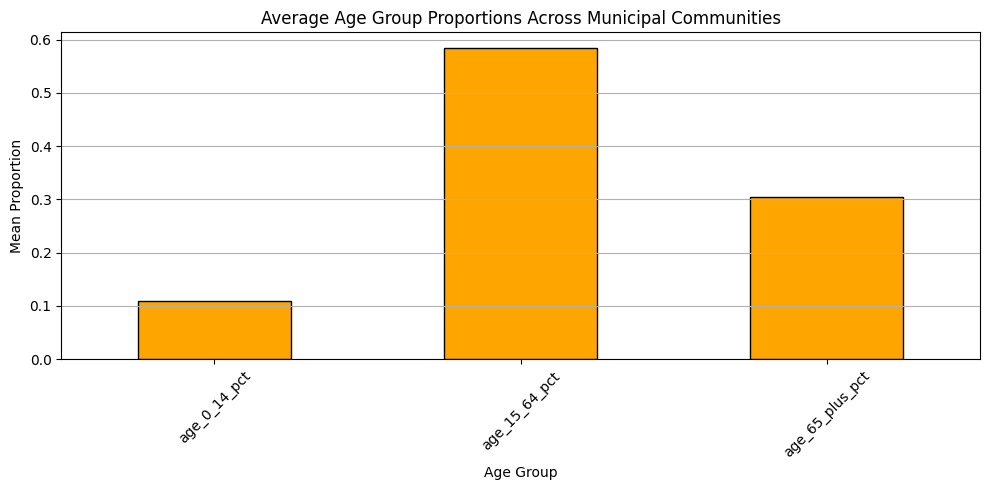
\includegraphics[scale=0.45]{figures/barchart_age_group_means.png}
    \centering
    \caption{Mean Age Group Features Bar Chart}
    \label{fig:bar_age_mean}
\end{figure}

\begin{figure}[!htbp]
    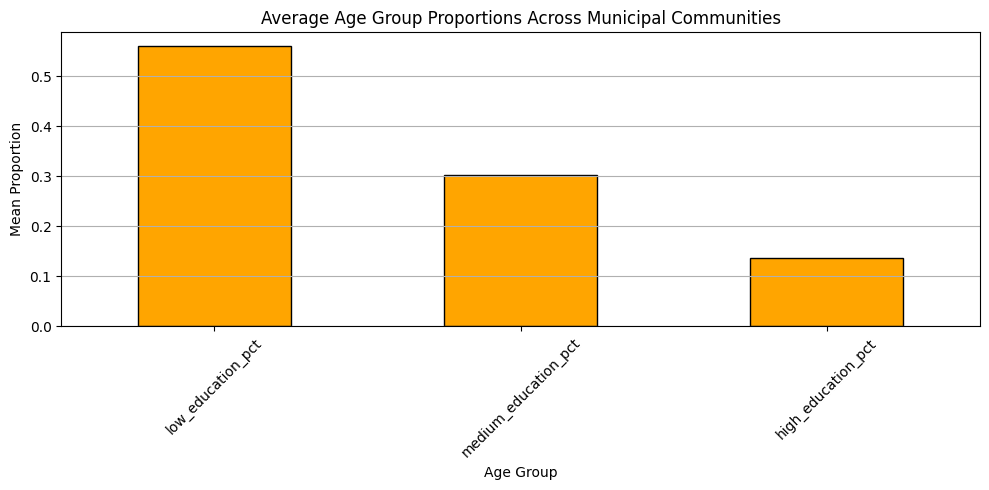
\includegraphics[scale=0.45]{figures/barchart_education_group_means.png}
    \centering
    \caption{Mean Education Group Features Bar Chart}
    \label{fig:bar_education_mean}
\end{figure}

\begin{figure}[!htbp]
    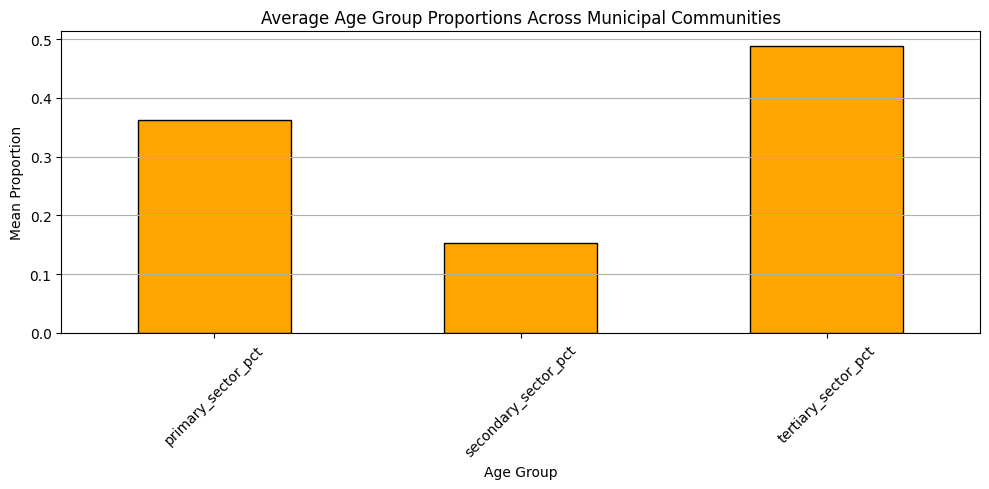
\includegraphics[scale=0.45]{figures/barchart_sector_group_means.png}
    \centering
    \caption{Mean Sector Group Features Bar Chart}
    \label{fig:bar_sector_mean}
\end{figure}


%========================================
\subsubsection{Scatter Plots}

\begin{figure}[h]
    \centering
    \begin{minipage}[b]{0.47\textwidth}
        \centering
        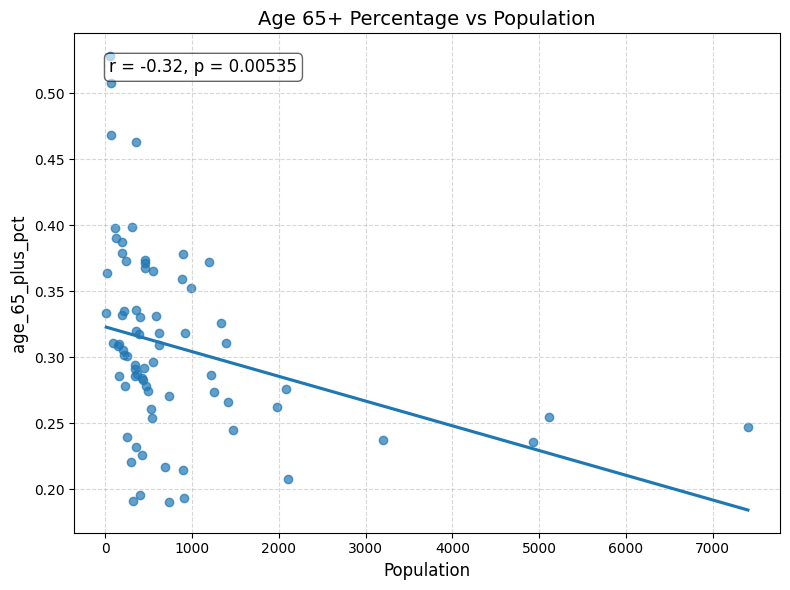
\includegraphics[height=5cm]{figures/scatter_population_elderly.png}
        \caption{Population VS Age 65+}
        \label{fig:scat_pop_elderly}
    \end{minipage}
    \hfill
    \begin{minipage}[b]{0.47\textwidth}
        \centering
        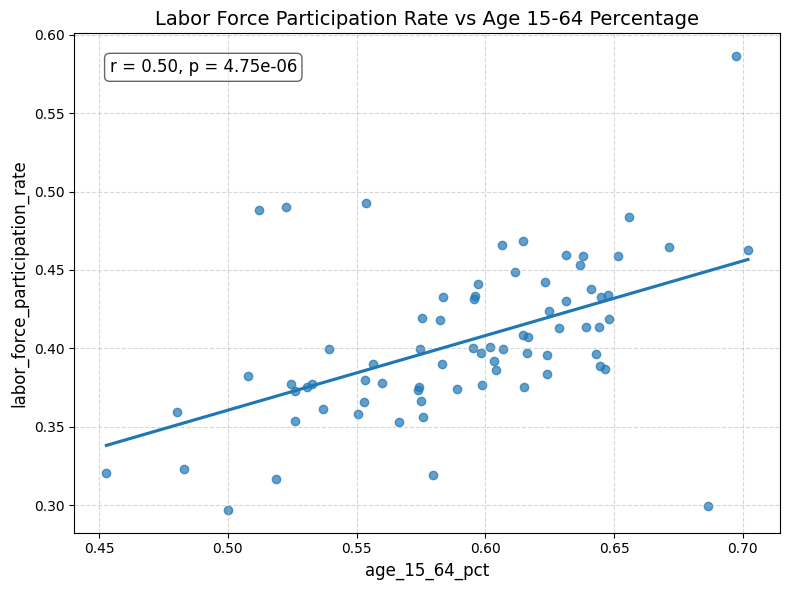
\includegraphics[height=5cm]{figures/scatter_labor_working.png}
        \caption{Labor Force VS Age 15-64 }
        \label{fig:scat_labor_working}
    \end{minipage}
\end{figure}


%========================================
\subsubsection{Correlation Matrices}
\label{sec:correlation_matrices} 

\begin{figure}[!htbp]
    \centering
    \begin{minipage}[b]{0.47\textwidth}
        \centering
        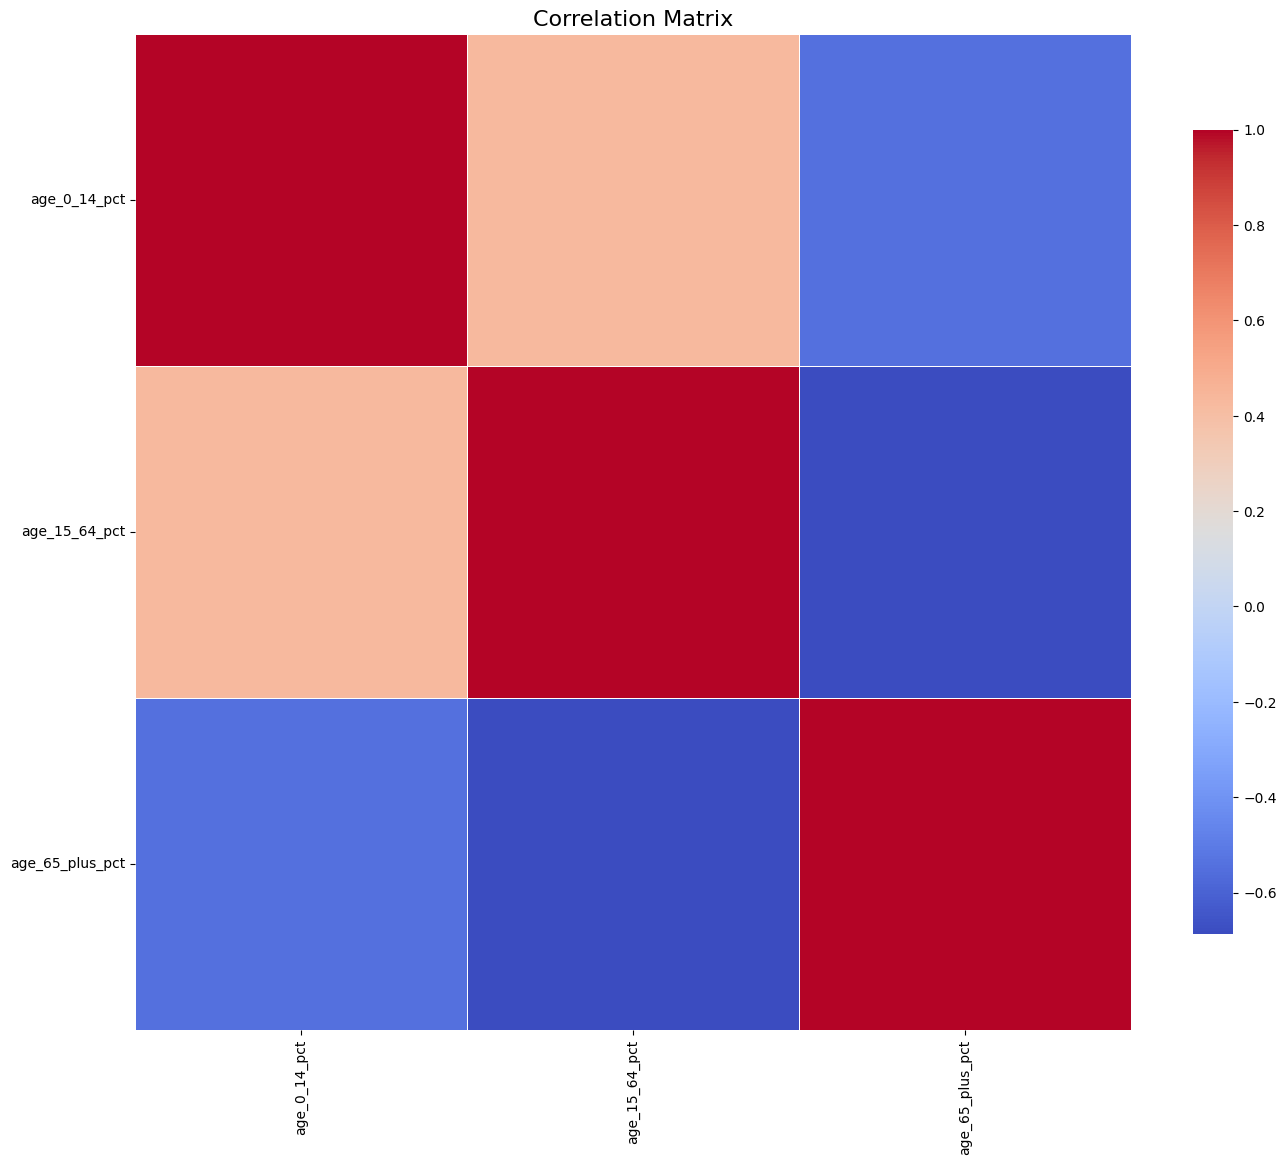
\includegraphics[height=5cm]{figures/corr_age.png}
        \caption{Age Groups}
        \label{fig:corr_age}
    \end{minipage}
    \hfill
    \begin{minipage}[b]{0.47\textwidth}
        \centering
        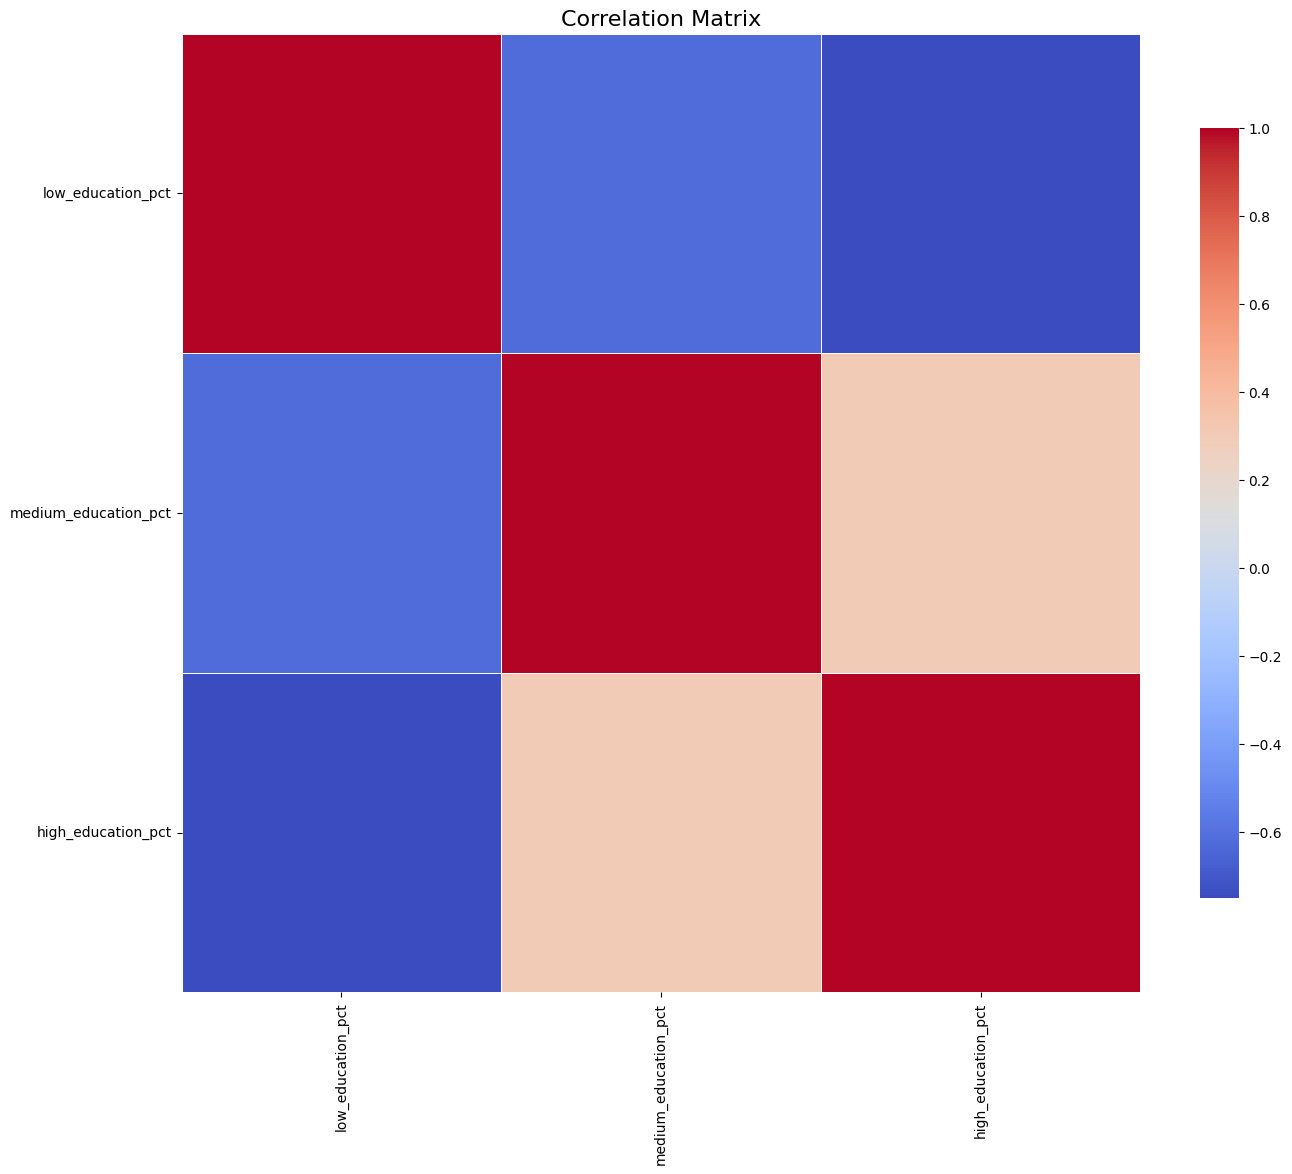
\includegraphics[height=5cm]{figures/corr_education.png}
        \caption{Educational Level Groups}
        \label{fig:corr_education}
    \end{minipage}
\end{figure}

\begin{figure}[!htbp]
    \centering
    \begin{minipage}[b]{0.47\textwidth}
        \centering
        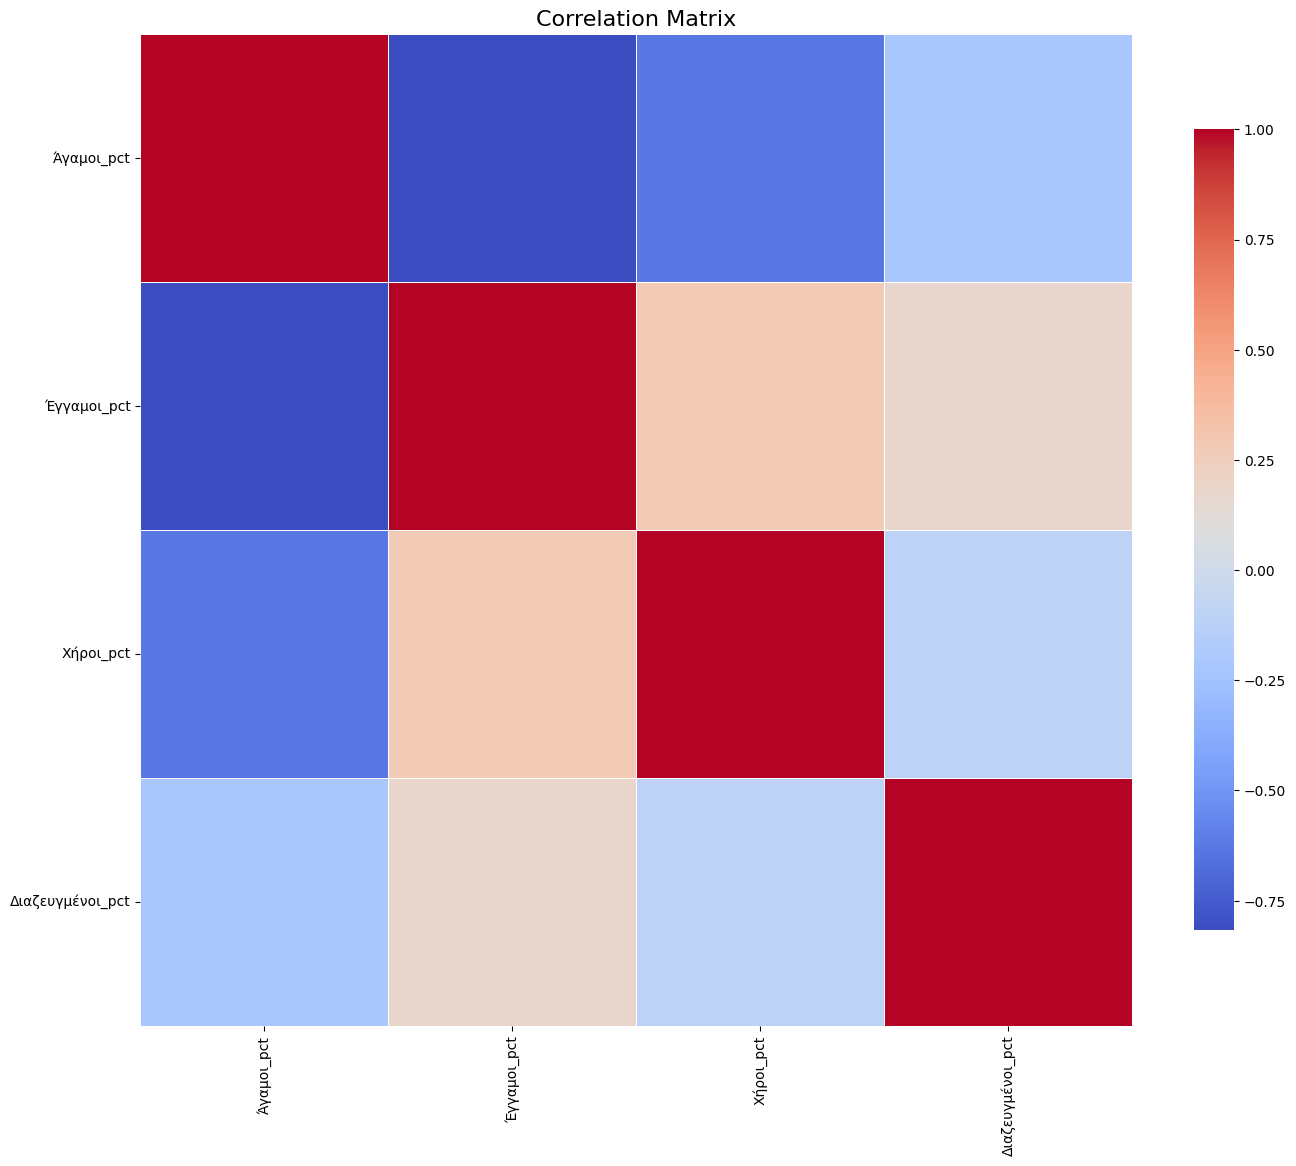
\includegraphics[height=5cm]{figures/corr_marriage.png}
        \caption{Martial Status Groups}
        \label{fig:corr_marriage}
    \end{minipage}
    \hfill
    \begin{minipage}[b]{0.47\textwidth}
        \centering
        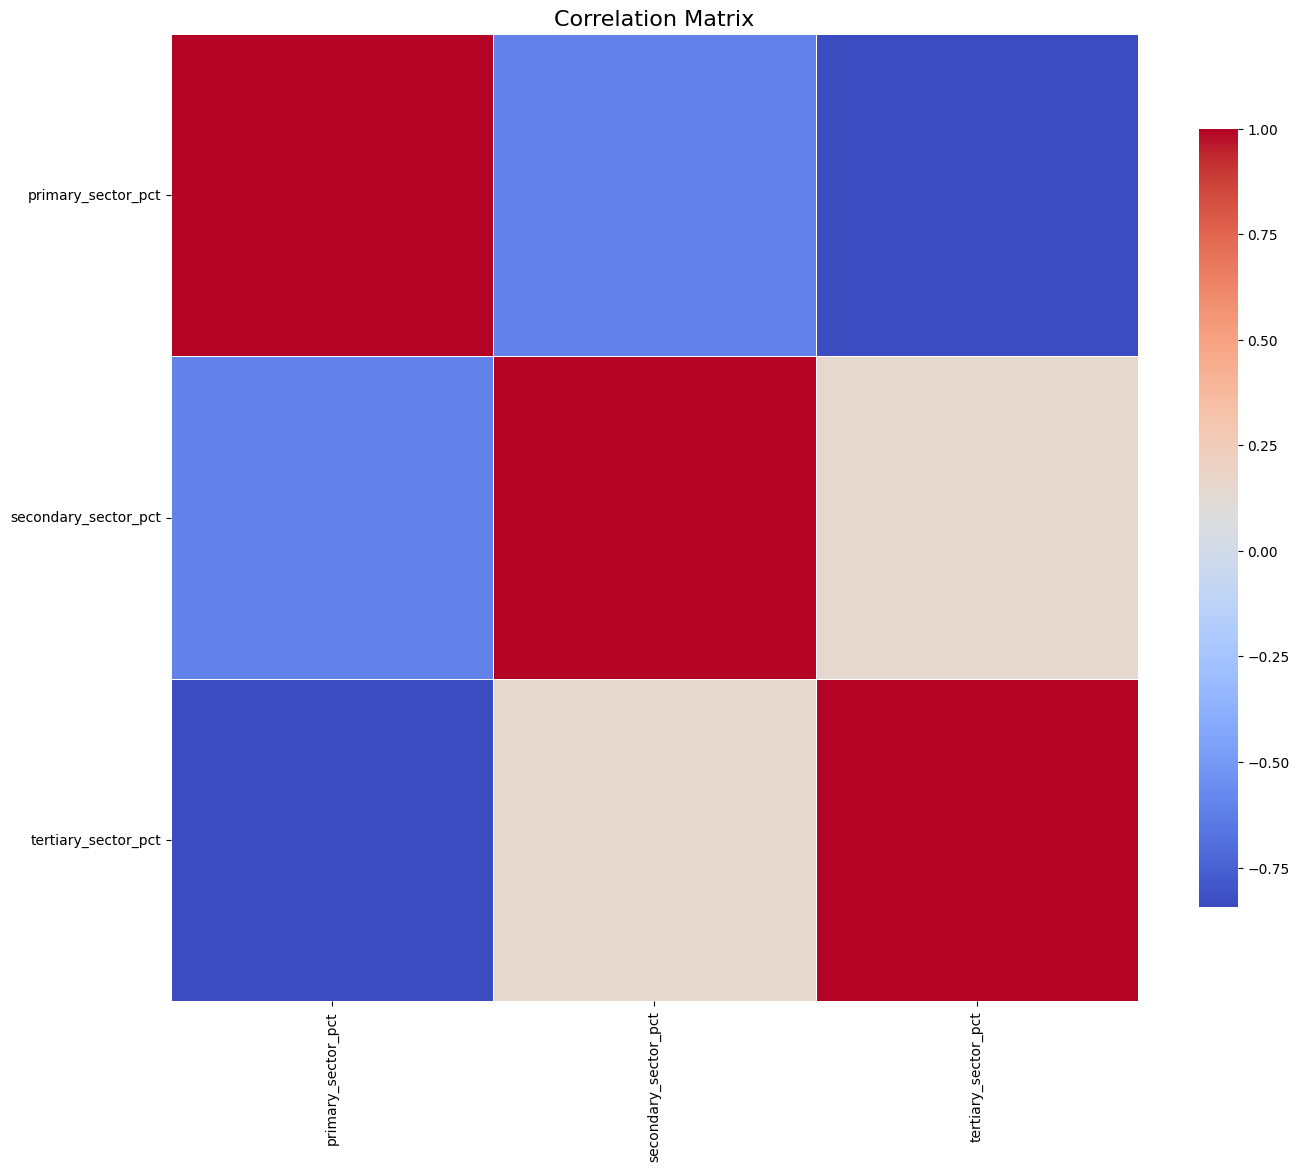
\includegraphics[height=5cm]{figures/corr_sector.png}
        \caption{Sector Groups}
        \label{fig:corr_sector}
    \end{minipage}
\end{figure}


%========================================
\subsubsection{Feature Engineering}
\label{sec:elstat_feature_engineering}

Below is presented the specific modifications performed in the feature groups in order to reduce the dimensionality:

\begin{itemize}
    \item Age Groups: 
        \begin{itemize}
            \item $age\_0\_14\_pct = (0-4)_{\%} + (5-9)_{\%} + (10-14)_{\%}$ (younger people)
            \item $age\_15\_64\_pct = (15-19)_{\%} + (20-24)_{\%} + (25-29)_{\%} + (30-34)_{\%} + (35-39)_{\%} + (40-44)_{\%} + (45-49)_{\%} + (50-54)_{\%} + (55-59)_{\%} + (60-64)_{\%}$ (working people)
            \item $age\_65\_plus\_pct = (65-69)_{\%} + (70-74)_{\%} + (75+)_{\%}$ (elderly people)
        \end{itemize}

    \item Educational Level Groups:
        \begin{itemize}
            \item $low\_education\_pct = no\_formal\_education_{\%} + primary\_education_{\%} + lower\_secondary_{\%}$
            \item $medium\_education\_pct = high\_school_{\%} + post\_secondary\_non\_uni_{\%}$
            \item $high\_education\_pct = higher\_education_{\%}$
        \end{itemize}

    \item Economic Hierarchical Features:
        \begin{itemize}
            \item $unemployment\_rate = \frac{\text{Άνεργοι}}{\text{Οικονομικά ενεργοί}}$
            \item $labor\_force\_participation\_rate = \frac{\text{Οικονομικά ενεργοί}}{\text{Σύνολο}}$
            \item $primary\_sector\_pct = \frac{\text{Πρωτογενής}}{\text{Απασχολούμενοι}}$
            \item $secondary\_sector\_pct = \frac{\text{Δευτερογενής}}{\text{Απασχολούμενοι}}$
            \item $tertiary\_sector\_pct = \frac{\text{Τριτογενής}}{\text{Απασχολούμενοι}}$
        \end{itemize}
\end{itemize}




%========================================
%========================================
%========================================

\section{Neighborhoods Dataset}

This section provides information about the structure of the Neighborhoods Dataset after extracting additional features from QGIS:


%========================================
\subsection{Datasets Structure}

Here we present the structure of the neighborhood dataset. 

\begin{longtable}{p{5cm} p{10cm}}
    \caption{Neighborhood Dataset Columns (highlighted features are used for joining)} \label{tab:neighborhood_columns} \\
    \hline
    \textbf{Column Name} & \textbf{Description} \\
    \hline
    \endfirsthead
    
    \multicolumn{2}{c}{{\bfseries Table \thetable\ (continued)}} \\
    \hline
    \textbf{Column Name} & \textbf{Description} \\
    \hline
    \endhead
    
    \hline \multicolumn{2}{r}{{Continued on next page}} \\
    \endfoot
    
    \hline
    \endlastfoot
    
    Neighborhood\_Greek & Neighborhood name in Greek \\
    Neighborhood & Neighborhood name in English \\
    Centroid\_x & Longitude coordinate of the neighborhood centroid \\
    Centroid\_y & Latitude coordinate of the neighborhood centroid \\
    Neighborhood\_Area\_km2 & Total area of the neighborhood polygon in square kilometers \\
    Geometry & Polygon geometry representing the neighborhood boundary \\
    distance\_to\_volos\_center\_km & Distance from the neighborhood centroid to the Volos city center (km)\\
    distance\_to\_volos\_port\_km & Distance from the neighborhood centroid to the Volos port (km)\\
    dist\_to\_main\_road\_km & Distance from the neighborhood centroid to the nearest main road (km)\\
    dist\_to\_bus\_stop\_km & Distance from the neighborhood centroid to the nearest bus stop (km)\\
    dist\_to\_university\_km & Distance from the neighborhood centroid to the University of Thessaly (km)\\
    \rowcolor{yellow!20}
    Municipal Community & Administrative municipal community in which the neighborhood is located \\
\end{longtable}



%========================================
%========================================
\subsection{Dataset Analysis}

Below we show various visualizations that occured during the EDA of the neighborhood dataset.

%========================================

\subsubsection{Feature Values Distributions}
\FloatBarrier

\begin{figure}[!htbp]
    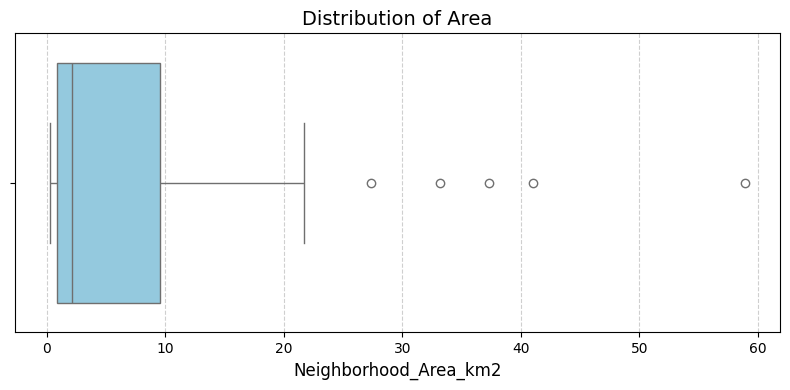
\includegraphics[scale=0.5]{figures/boxplot_area_neighbor.png}
    \centering
    \caption{'Neighborhood\_area\_km2' Feature Boxplot}
    \label{fig:box_area_neigh}
\end{figure}

\begin{figure}[!htbp]
    \centering
    \begin{subfigure}[b]{0.47\textwidth}
        \centering
        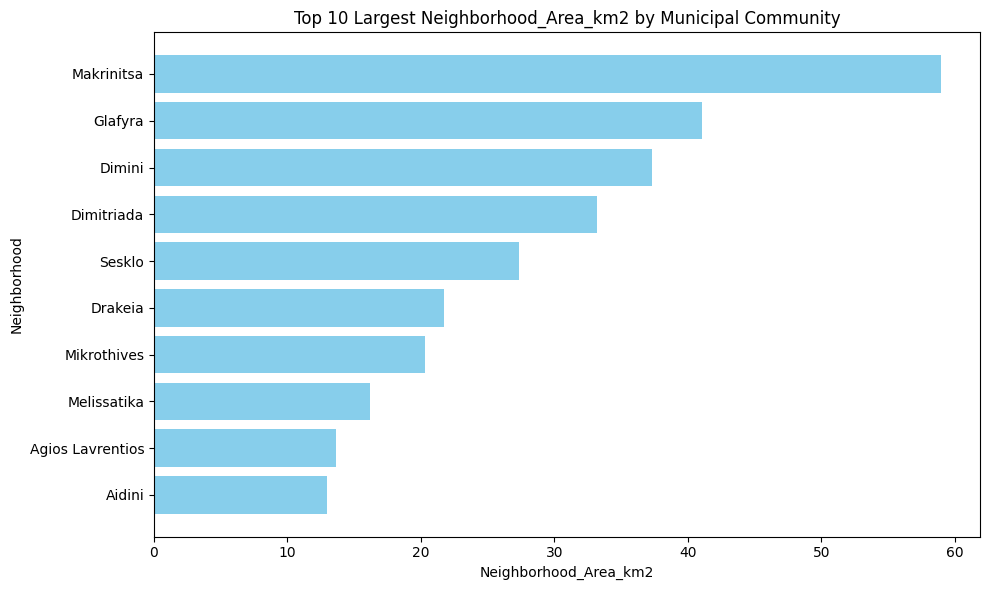
\includegraphics[height=5cm]{figures/barchart_area_neighborhood.png}
        \caption{Neighborhood area Bar Chart}
        \label{fig:bar_area_neigh}
    \end{subfigure}
    \hfill
    \begin{subfigure}[b]{0.47\textwidth}
        \centering
        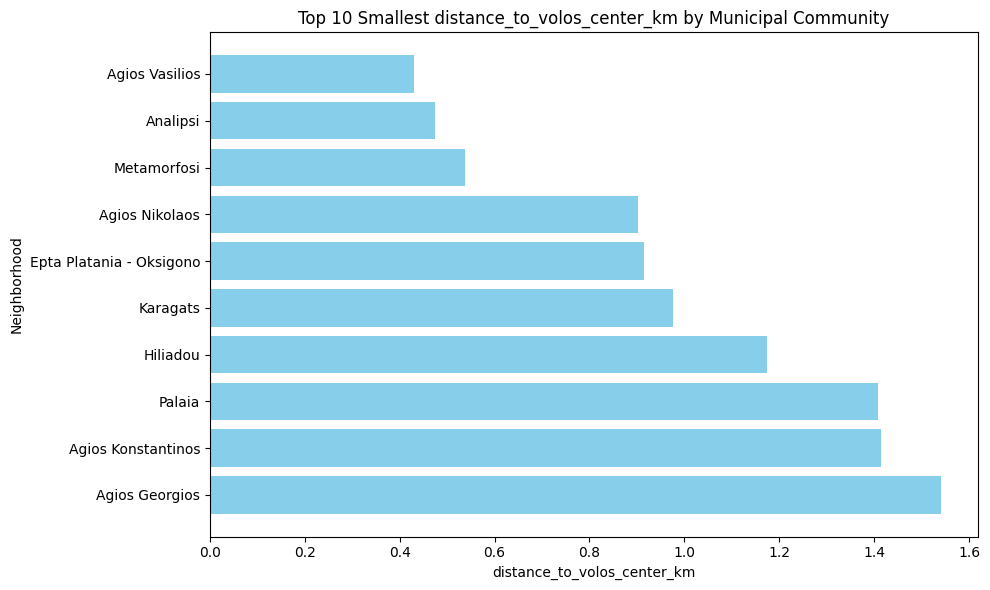
\includegraphics[height=5cm]{figures/barchart_center.png}
        \caption{'Distance to Center  Bar Chart}
        \label{fig:bar_center_neigh}
    \end{subfigure}
\end{figure}

%========================================
\newpage
\subsubsection{Scatter Plots}
\FloatBarrier

\begin{figure}[!htbp]
    \centering
    \begin{subfigure}[b]{0.47\textwidth}
        \centering
        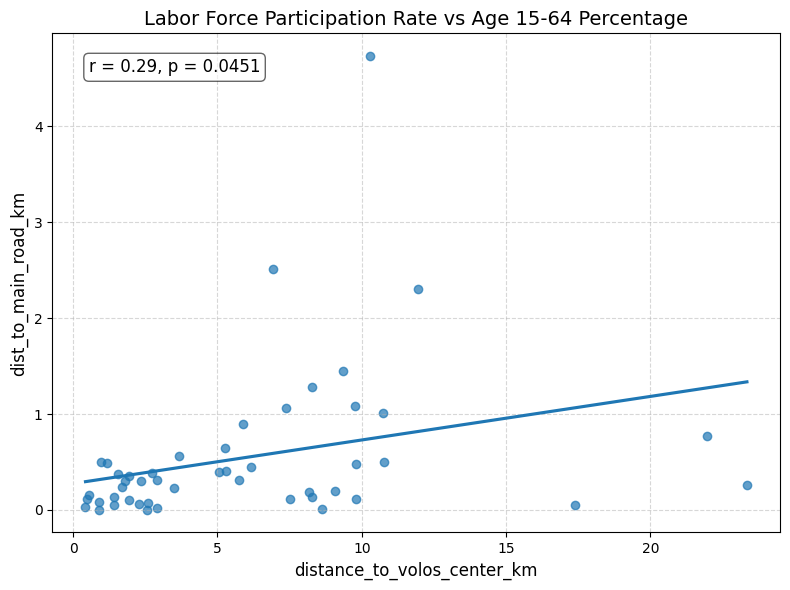
\includegraphics[height=5cm]{figures/scatter_center_highway.png}
        \caption{Distance from Center VS Distance from Main Roads}
        \label{fig:scatter_center_highway}
    \end{subfigure}
    \hfill
    \begin{subfigure}[b]{0.47\textwidth}
        \centering
        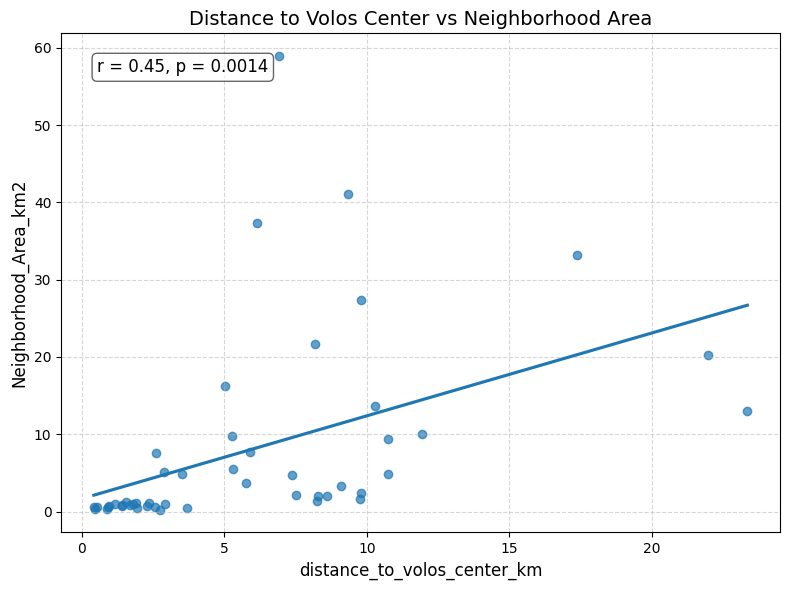
\includegraphics[height=5cm]{figures/scatter_center_area.png}
        \caption{Distance from Center VS Neighborhood Area}
        \label{fig:scatter_center_area}
    \end{subfigure}
\end{figure}





%========================================
%========================================
%========================================
\section{Joined Dataset}

This appendix contains information about the business dataset after joining it both with the neighborhood and municipal community features. 

%========================================
%========================================
\subsection{Dataset Structure}

This section provides the structure of the joined business dataset.

\begin{longtable}{p{5cm} p{10cm}}
    \caption{Joined Dataset Columns} \label{tab:business_joined_columns} \\
    \hline
    \textbf{Column Name} & \textbf{Description} \\
    \hline
    \endfirsthead
    
    \multicolumn{2}{c}{{\bfseries Table \thetable\ (continued)}} \\
    \hline
    \textbf{Column Name} & \textbf{Description} \\
    \hline
    \endhead
    
    \hline \multicolumn{2}{r}{{Continued on next page}} \\
    \endfoot
    
    \hline
    \endlastfoot
    
    Name & Business name as listed in the source dataset \\
    Category & General business category (e.g., restaurant, retail, service) \\
    Latitude & Geographic latitude coordinate of the business location \\
    Longitude & Geographic longitude coordinate of the business location \\
    Address & Full street address of the business \\
    Country & Country where the business is located \\
    City & City where the business is located \\
    Postal Code & Postal code of the business location \\
    Rating & Average rating score given by customers, if available \\
    Reviews & Number of customer reviews, if available \\
    Source & Origin of the business entry \\
    Description & Short textual description of the business \\
    NACE Code & Official NACE classification code for the business activity \\
    NACE Description (EN) & English description of the NACE code activity \\
    Municipal Community & The municipal community of the business location \\
    Neighborhood & The neighborhood of the business location \\
    ΠΕΡΙΦΕΡΕΙΑΚΗ ΕΝΟΤΗΤΑ & Greek regional unit where the business is located \\
    ΔΗΜΟΣ & Municipality where the business is located \\
    ΔΗΜΟΤΙΚΗ ΕΝΟΤΗΤΑ & Municipal unit of the business location \\
    Population & Total population of the municipal community \\
    Άγαμοι\_pct & Percentage of unmarried individuals in the population \\
    Έγγαμοι\_pct & Percentage of married individuals in the population \\
    Χήροι\_pct & Percentage of widowed individuals in the population \\
    Διαζευγμένοι\_pct & Percentage of divorced individuals in the population \\
    age\_0\_14\_pct & Percentage of population aged 0–14 \\
    age\_15\_64\_pct & Percentage of population aged 15–64 \\
    age\_65\_plus\_pct & Percentage of population aged 65 and older \\
    low\_education\_pct & Percentage of population with low education level \\
    medium\_education\_pct & Percentage of population with medium education level \\
    high\_education\_pct & Percentage of population with high education level \\
    unemployment\_rate & Unemployment rate in the municipal community \\
    labor\_force\_participation\_rate & Labor force participation rate in the municipal community \\
    primary\_sector\_pct & Employment percentage in the primary sector\\ 
    secondary\_sector\_pct & Employment percentage in the secondary sector \\
    tertiary\_sector\_pct & Employment percentage in the tertiary sector \\
    Area\_km2 & Total area of the municipal community in square kilometers \\
    Neighborhood\_Area\_km2 & Total area of the neighborhood in square kilometers \\
    distance\_to\_volos\_center\_km & Distance from the neighborhood center to Volos city center (km) \\
    distance\_to\_volos\_port\_km & Distance from the neighborhood center to Volos port (km) \\
    dist\_to\_main\_road\_km & Distance from the neighborhood center to the nearest main road (km) \\
    dist\_to\_bus\_stop\_km & Distance from the neighborhood center to the nearest bus stop (km) \\
    dist\_to\_university\_km & Distance from the neighborhood center to the nearest university (km) \\
\end{longtable}


%========================================
%========================================
\subsection{Missing Data Analysis}

Here we present a heatmap of the missing values across all the features of the joined dataset.

\begin{figure}[h]
    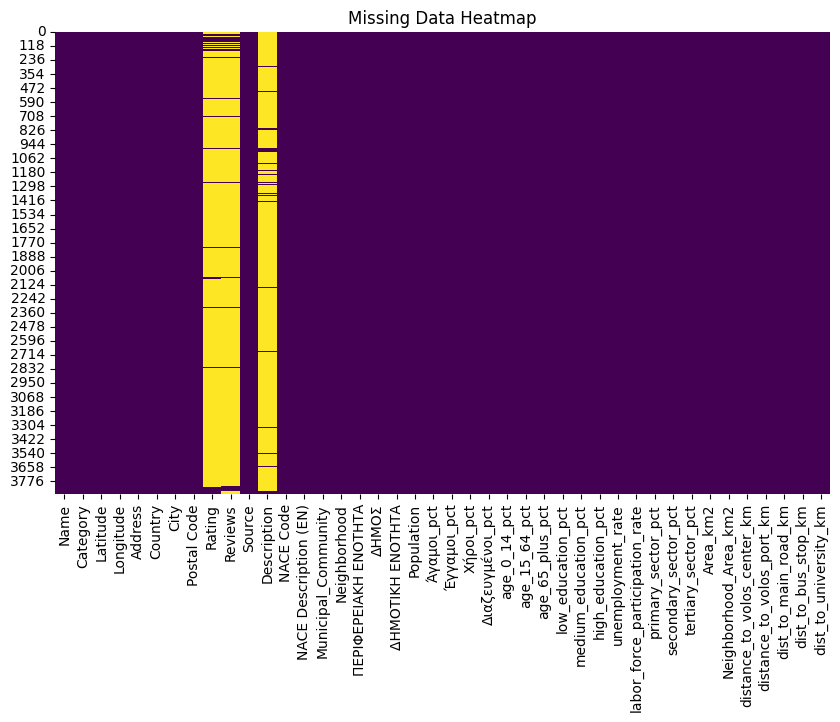
\includegraphics[scale=0.45]{figures/heatmap_missing.png}
    \centering
    \caption{Missing Data Heatmap}
    \label{fig:heatmap_missing}
\end{figure}



%========================================
%========================================
%========================================
\section{Proxy Ground Truths}
\label{venn_diagrams}


This appendix contains information about the procedure of creating the proxy ground truths. Below we present some indicative Venn diagrams of the agreement count between the three different proxy truth creation methods. Not every single one will be shown since their total number is 306 (1 per NACE class).


\begin{figure}[h]
    \centering
    \begin{minipage}[b]{0.47\textwidth}
        \centering
        
\includegraphics[height=5cm]{figures/venn_nace_47_25.png}
        \caption{Venn Diagram for NACE Class 47.25 (Partial Similarity)}
        \label{fig:venn_nace_47_25}
    \end{minipage}
    \hfill
    \begin{minipage}[b]{0.47\textwidth}
        \centering
        
\includegraphics[height=5cm]{figures/venn_nace_28_49.png}
        \caption{Venn Diagram for NACE Class 28.49 (Perfect Similarity)}
        \label{fig:venn_nace_28_49}
    \end{minipage}
\end{figure}

 

%
%%%%%%%%%%%%%%%%%%%%%%%%%%%%%%%%%%%%%%%%%%%%%%%%%%%%


\end{document}